In this section, we study the identification of boosted top quarks at Run II of the LHC. Boosted top quarks result in large-radius jets with complex substructure, containing a $b$-subjet and a boosted $W$. The additional kinematic handles coming from the reconstruction of the $W$ mass and $b$-tagging allows a very high degree of discrimination of top quark jets from QCD backgrounds. 

We consider top quarks with moderate boost (600-1000 GeV), and perhaps most interestingly, at high boost ($\gtrsim1500$ GeV). Top tagging faces several challenges in the high-$\pt$ regime. For such high-$\pt$ jets, the $b$-tagging efficiencies are no longer reliably known. Also, the top jet can also accompanied by additional radiation with $\pt\sim m_t$, leading to combinatoric ambiguities of reconstructing the top and $W$, and the possibility that existing taggers or observables shape the background by looking for subjet combinations that reconstruct $m_t$/$m_W$. To study this, we examine the performance of both mass-reconstruction variables, as well as shape observables that probe the three-pronged nature of the top jet and the accompanying radiation pattern.

\subsection{Methodology}
We study a number of top-tagging strategies, in particular:
%
\begin{enumerate}
\item HEPTopTagger
\item Johns Hopkins Tagger (JH)
\item Trimming
\item Pruning
\end{enumerate}
%
The top taggers have criteria for reconstructing a top and $W$ candidate, while the grooming algorithms (trimming and pruning) do not incorporate a $W$-identification step. For a level playing field, we construct a $W$ candidate from the three leading subjets by taking the pair of subjets with the smallest invariant mass; in the case that only two subjets are reconstructed, we take the mass of the leading subjet. All of the above taggers and groomers incorporate a step to remove pile-up and other soft radiation.

We also consider the performance of jet shape observables. In particular, we consider the $N$-subjettiness ratios $\tau_{32}^{\beta=1}$ and $\tau_{21}^{\beta=1}$, energy correlation function ratios $C_3^{\beta=1}$ and $C_2^{\beta=1}$, and the Qjet mass volatility $\Gamma$. In addition to the jet shape performance, we combine the jet shapes with the mass-reconstruction methods listed above to determine the optimal combined performance.

To quantify the performance of each set of variables, we combine the relevant tagger output observables and/or jet shapes into a boosted decision tree (BDT), which determines the optimal multivariable cut. Additionally, because each tagger has two inputs (list, or maybe refer back to Section 3), we scan over reasonable values of the inputs to determine the optimal value for each top tagging signal efficiency. This allows  a direct comparison of the optimized version of each tagger. The input values scanned for the various algorithms are:
%
\begin{itemize}
\item {\bf HEPTopTagger:} $m\in[30,100]$ GeV, $\mu\in[0.5,1]$
\item {\bf JH Tagger:} $\delta_p\in[0.02,0.15]$, $\delta_R\in[0.07,0.2]$
\item {\bf Trimming:} $f_{\rm cut}\in[0.02,0.14]$, $R_{\rm trim}\in[0.1,0.5]$
\item {\bf Pruning:} $z_{\rm cut}\in[0.02,0.14]$, $D_{\rm cut}\in[0.1,0.6]$
\end{itemize}

\subsection{Single-observable performance}
We start by investigating the behavior of individual jet substructure observables. Because of the rich, three-pronged structure of the top decay, it is expected that combinations of masses and jet shapes will far outperform single observables in identifying boosted tops. However, a study of the top-tagging performance of single variables facilitates a direct comparison with the $W$ tagging results in Section \ref{sec:wtagging}, and also allows a straightforward examination of the performance of each observable for different $\pt$ and jet radius.

Fig.~\ref{fig:single_variable_ROC} shows the ROC curves for each of the top-tagging observables, with the bare jet mass also plotted for comparison. Unlike $W$ tagging, the jet shape observables perform more poorly than jet mass. \emph{(Check reasoning: this argument due to Andrew Larkoski)}. As an example illustrating why this is the case, consider $N$-subjettiness. The $W$ is two-pronged and the top is three-pronged; therefore, we expect $\tau_{21}$ and $\tau_{32}$ to be the best-performant $N$-subjettiness ratio, respectively. However, $\tau_{21}$ also contains an implicit cut on the denominator, $\tau_1$, which is strongly correlated with jet mass. Therefore, $\tau_{21}$ combines both mass and shape information to some extent. By contrast, and as is clear in Fig.\ref{fig:single_variable_ROC}(a), the best shape for top tagging is $\tau_{32}$, which contains no information on the mass. Therefore, it is  unsurprising that the  shapes most useful for top tagging are less sensitive to the jet mass, and under-perform relative to the corresponding observables for $W$ tagging.

\begin{figure*}
\begin{center}
\subfigure[Jet shapes]{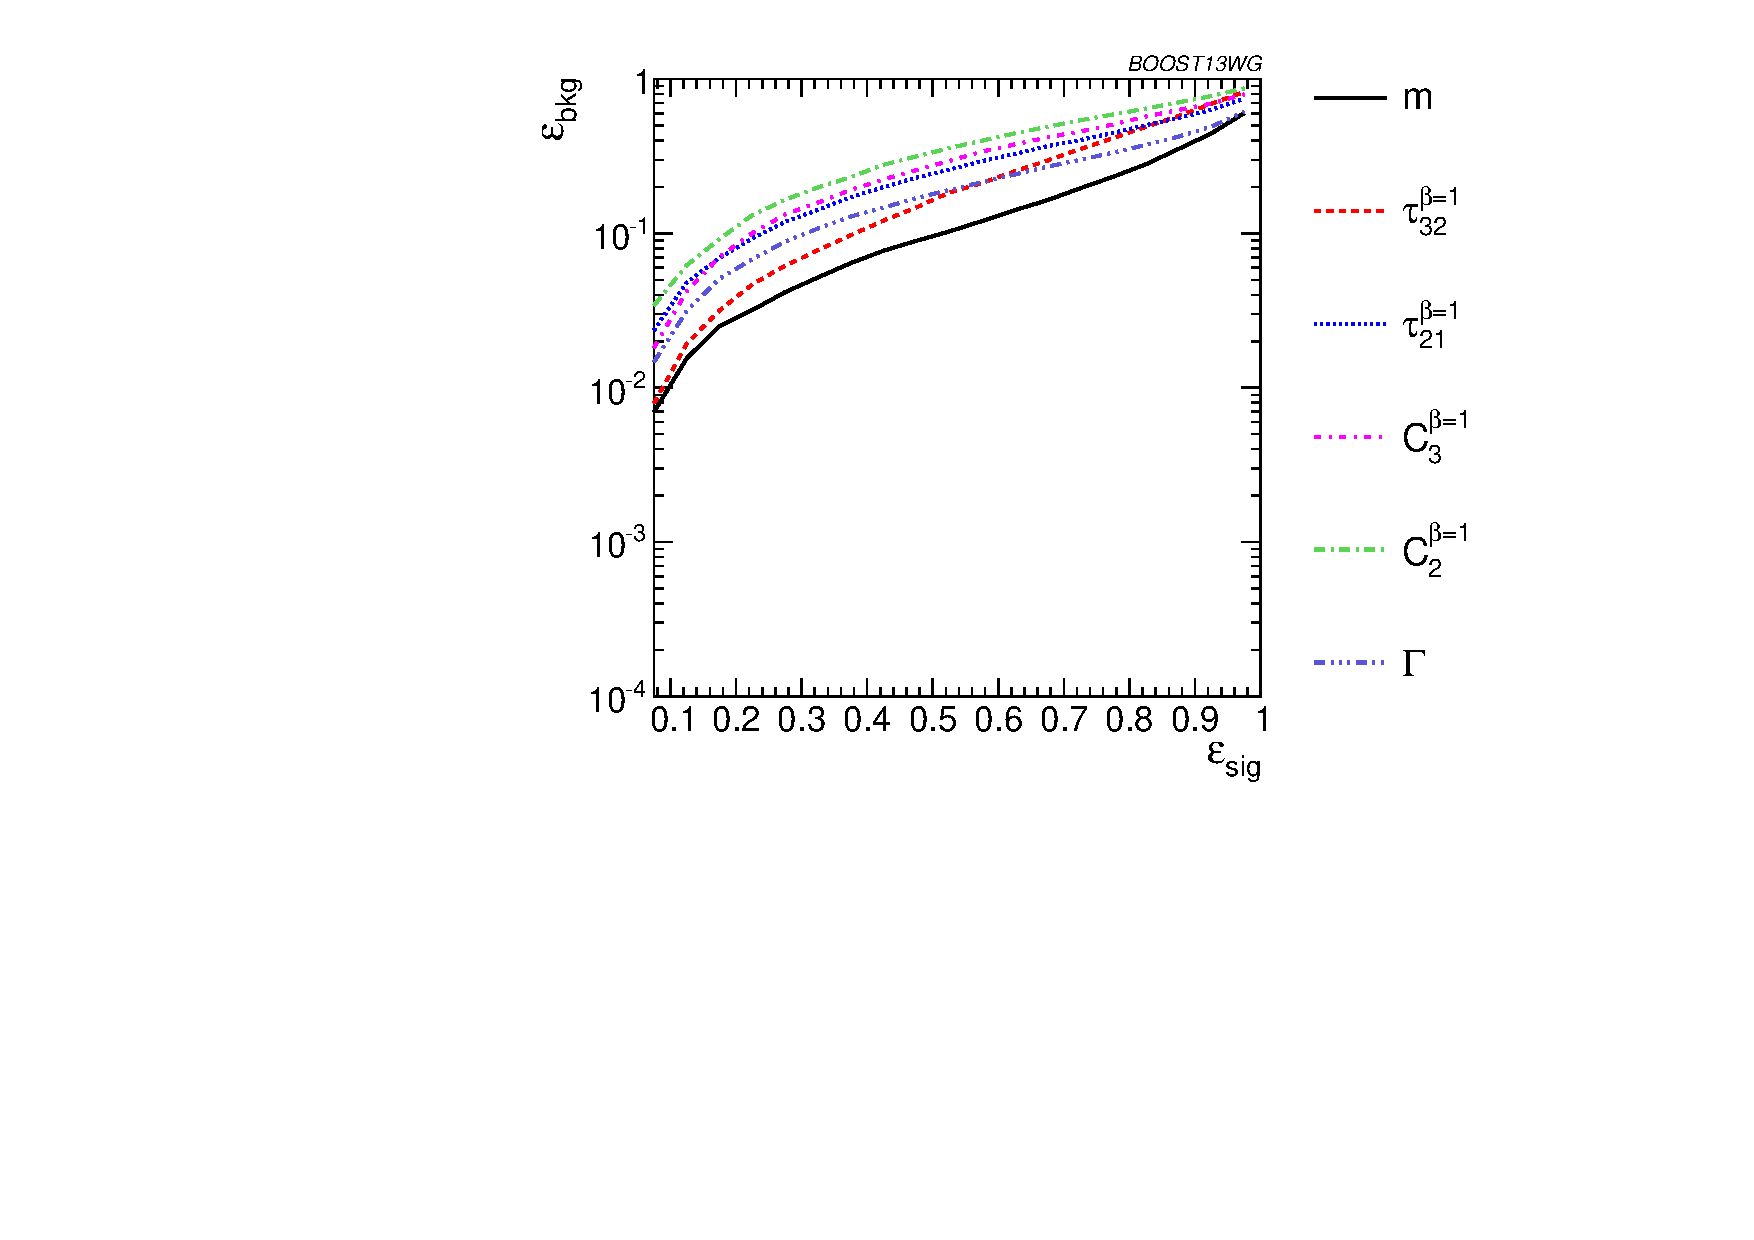
\includegraphics[width=0.48\textwidth]{./Figures/TTagging/single_variable/pT.1TeV.R.0.8/Rocs_shape.pdf}}
\subfigure[Top mass]{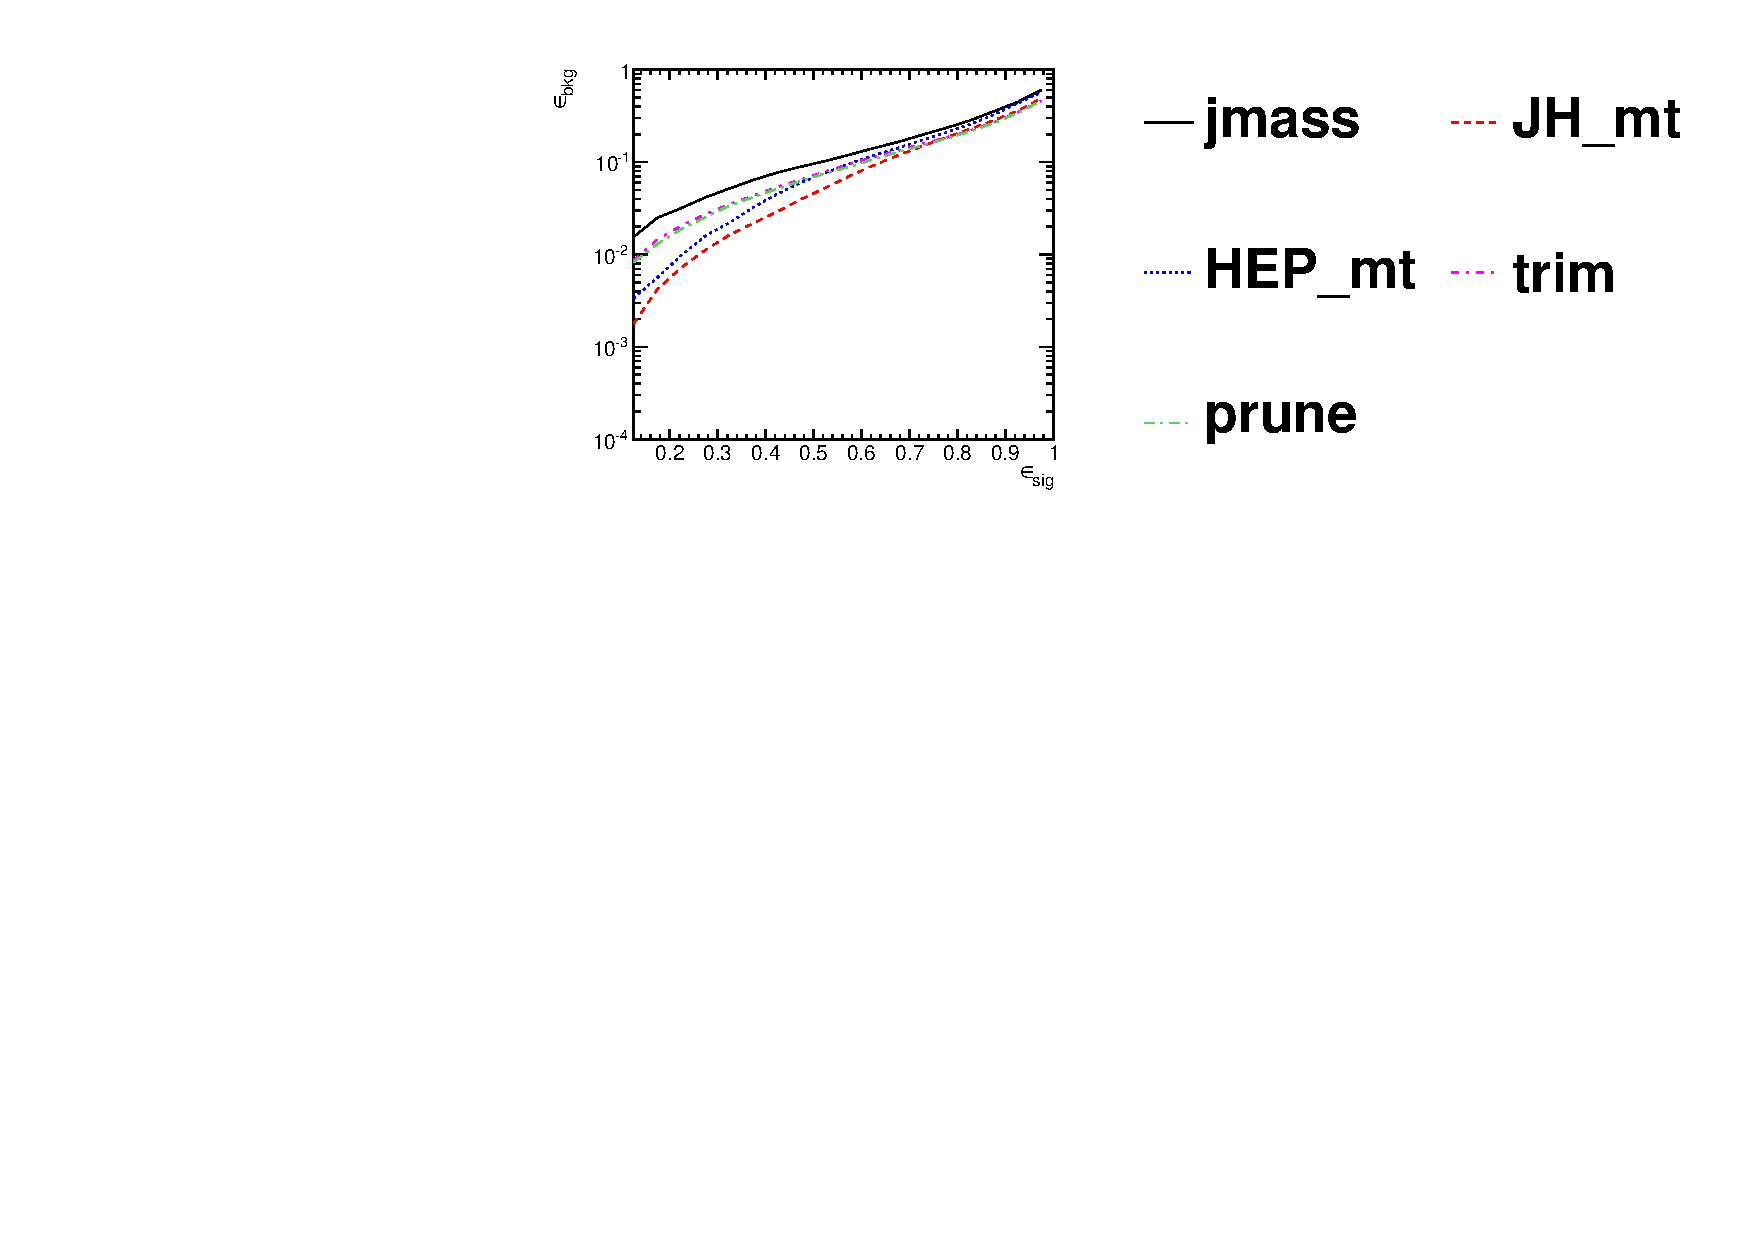
\includegraphics[width=0.48\textwidth]{./Figures/TTagging/single_variable/pT.1TeV.R.0.8/Rocs_top_mass.pdf}}
\subfigure[$W$ mass]{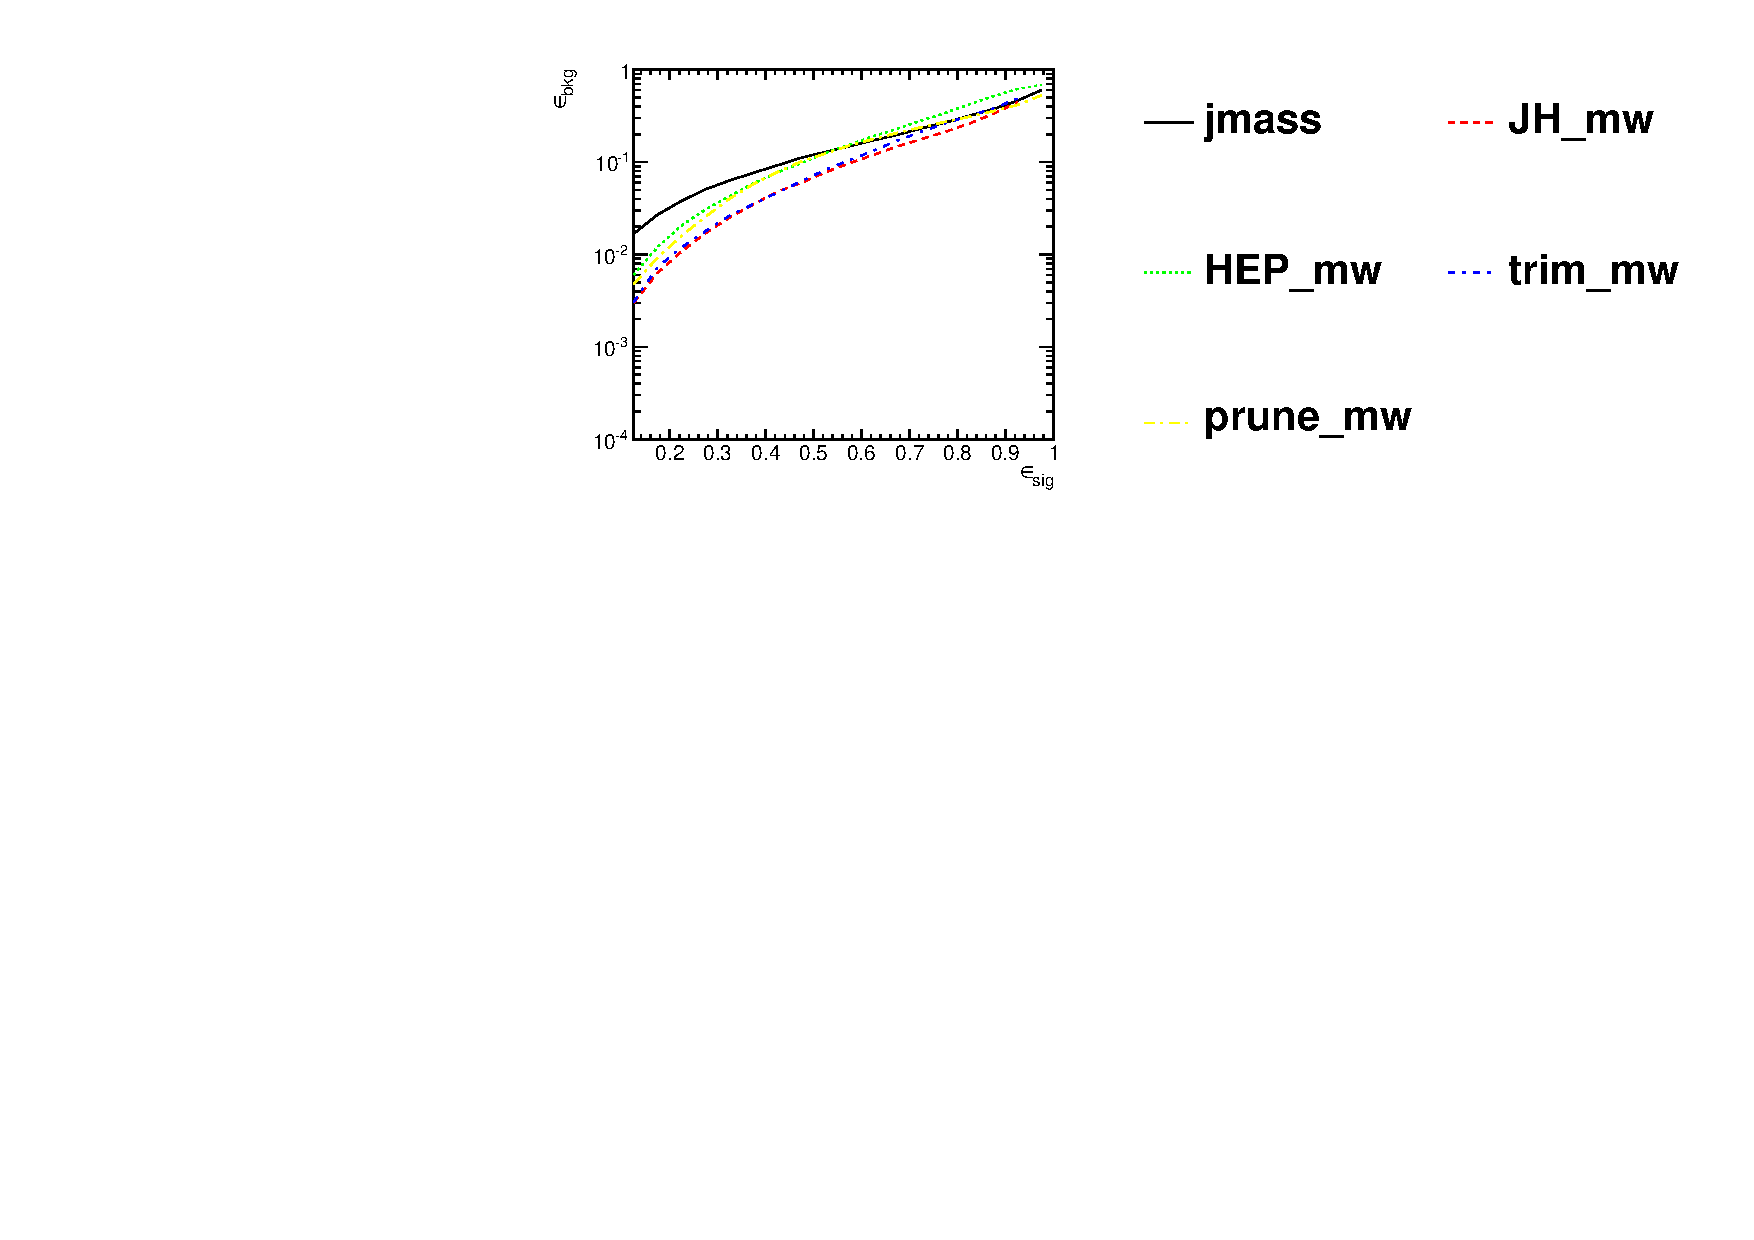
\includegraphics[width=0.48\textwidth]{./Figures/TTagging/single_variable/pT.1TeV.R.0.8/Rocs_w_mass.pdf}}
\caption{Comparison of single-variable top-tagging performance in the \pt 1000-1100 GeV bin using the anti-\kT, R=0.8 algorithm.}
\label{fig:single_variable_ROC}
\end{center}
\end{figure*}

Of the two top tagging algorithms, the Johns Hopkins (JH) tagger out-performs the HEPTopTagger in its signal-to-background separation of both the top and $W$ candidate masses, with larger discrepancy at higher $\pt$ and larger jet radius. In Fig.~\ref{fig:topmass_histogram_HEP_JH}, we show the histograms for the top mass output from the JH and HEPTopTagger for different $\pt$ and $R$, optimized at a signal efficiency of 30\%. The likely reason for this behavior is that, in the HEPTopTagger algorithm, the jet is filtered to select the five hardest subjets, and then three subjets are chosen which reconstruct the top mass. This requirement tends to shape a peak in the QCD background around $m_t$ for the HEPTopTagger, while the JH tagger has no such requirement. It has been suggested by Anders \emph{et al.} \cite{Anders:2013oga} that performance in the HEPTopTagger may be improved by selecting the three subjets reconstructing the top only among those that pass the $W$ mass constraints, which somewhat reduces the shaping of the background. \emph{Maybe try this out with my code to see if it helps?}

\begin{figure*}
\begin{center}
\subfigure[Johns Hopkins Tagger, $R=0.4$]{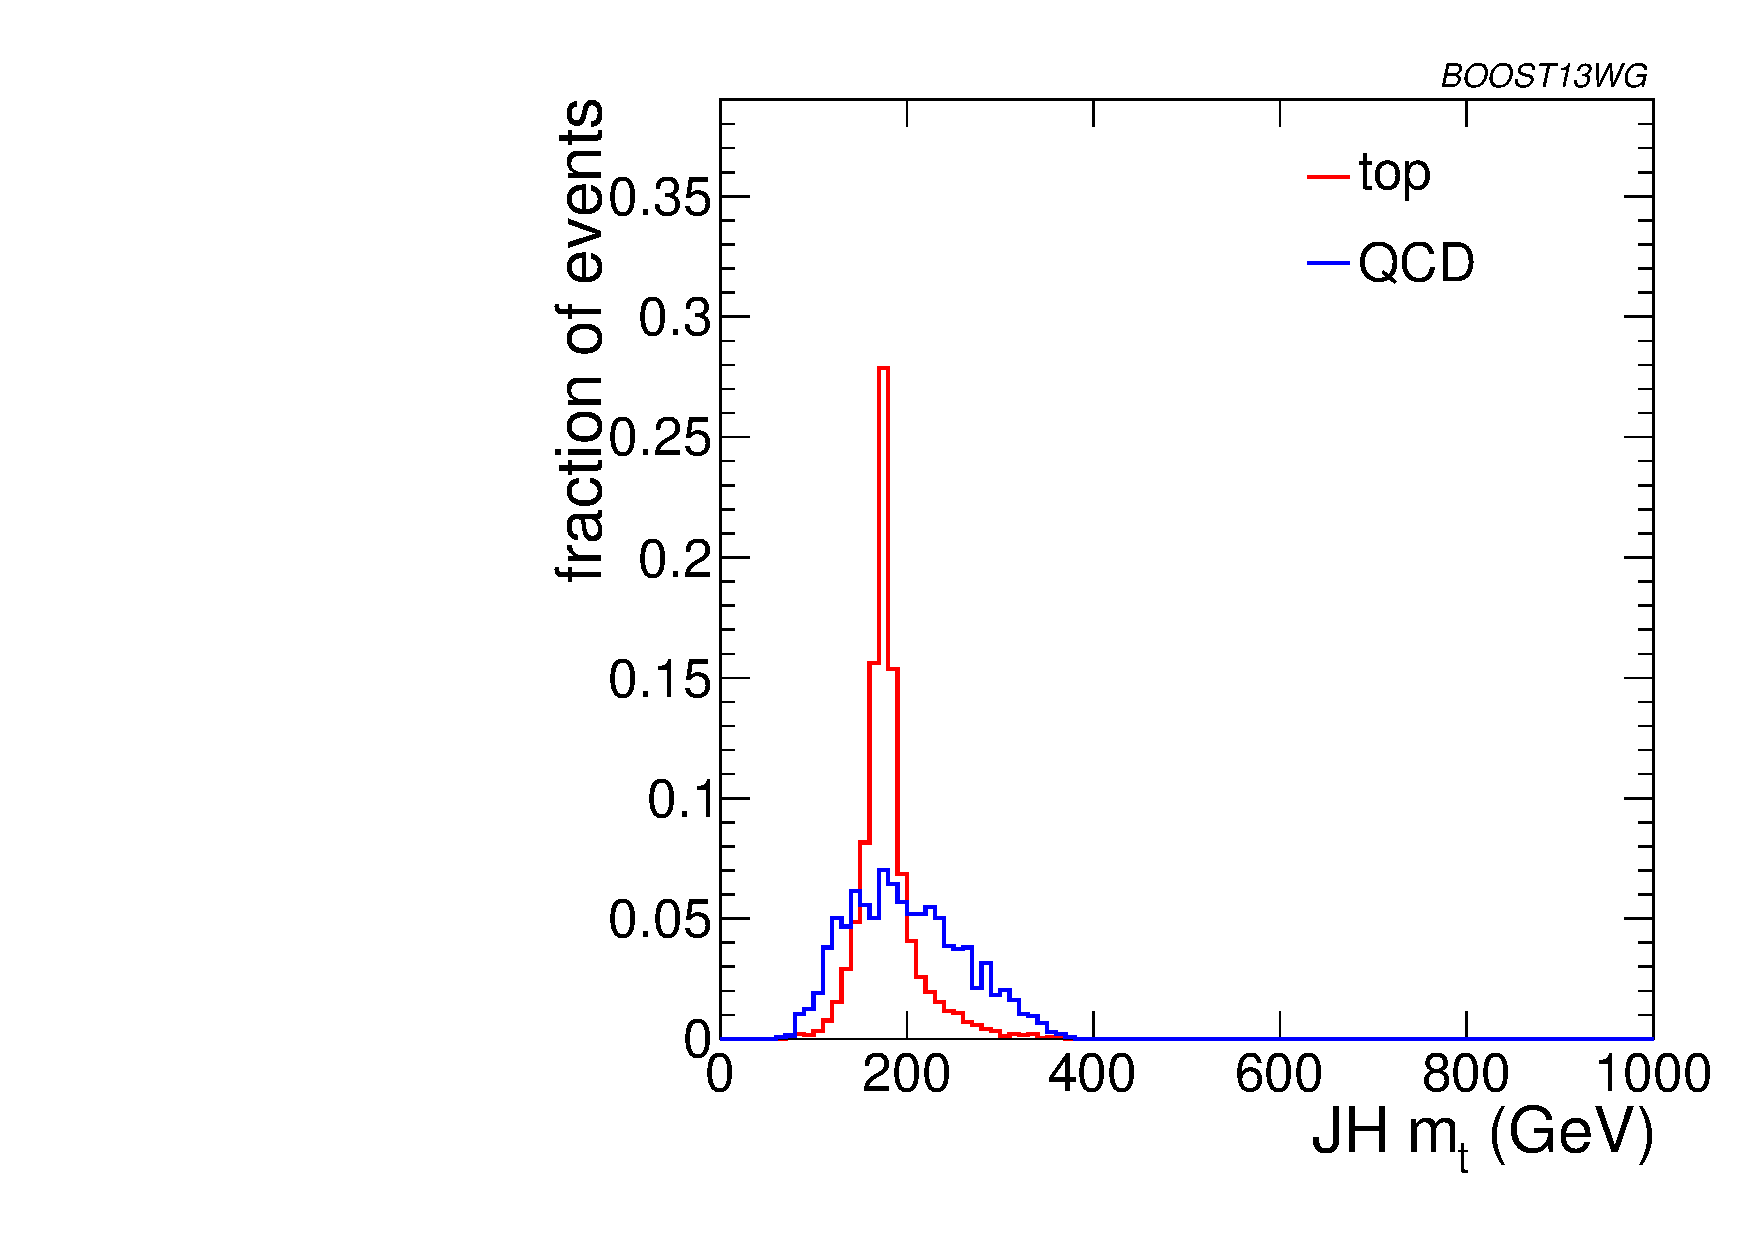
\includegraphics[width=0.48\textwidth]{./Figures/TTagging/single_variable/pT.1.5TeV.R.0.4/h_JH_mt_opt_mt.pdf}}
\subfigure[HEPTopTagger, $R=0.4$]{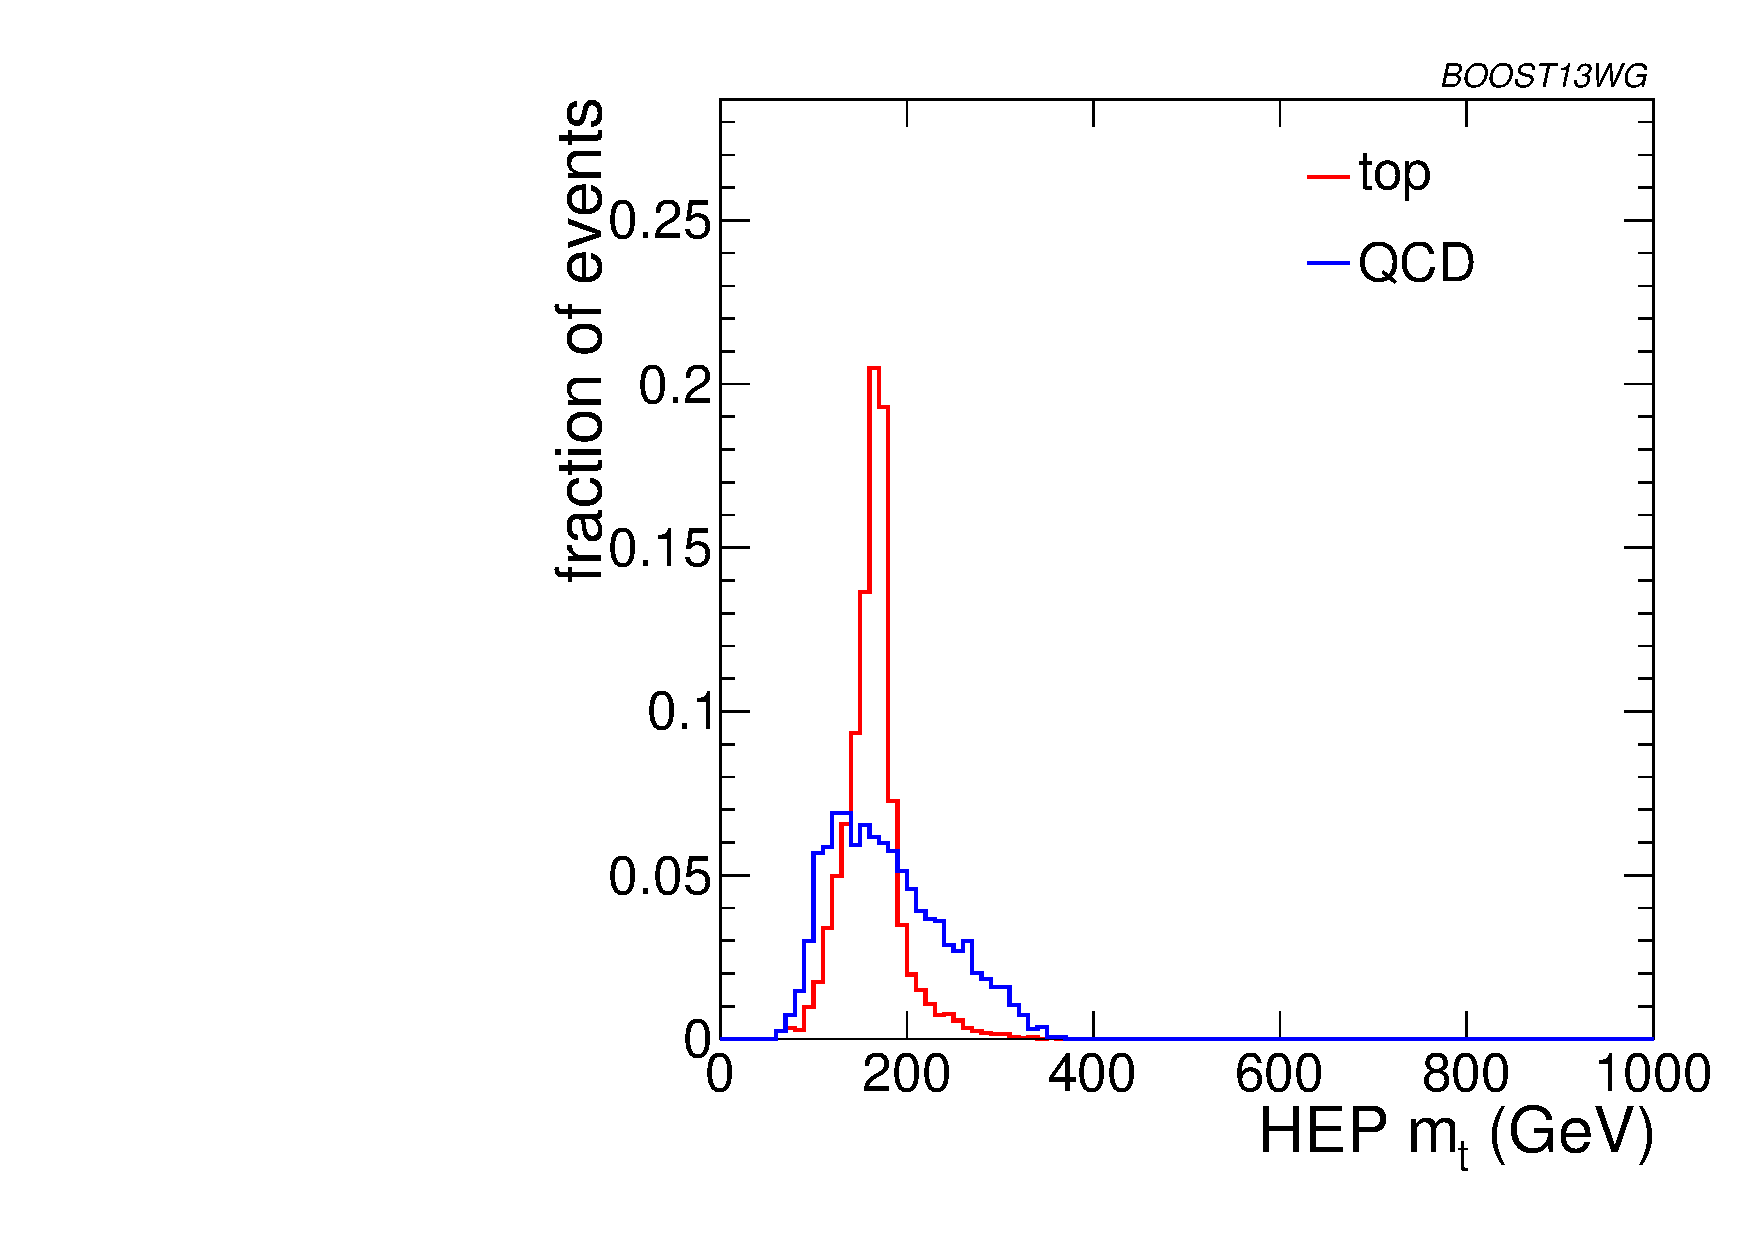
\includegraphics[width=0.48\textwidth]{./Figures/TTagging/single_variable/pT.1.5TeV.R.0.4/h_HEP_mt_opt_mt.pdf}}
\subfigure[Johns Hopkins Tagger, $R=0.8$]{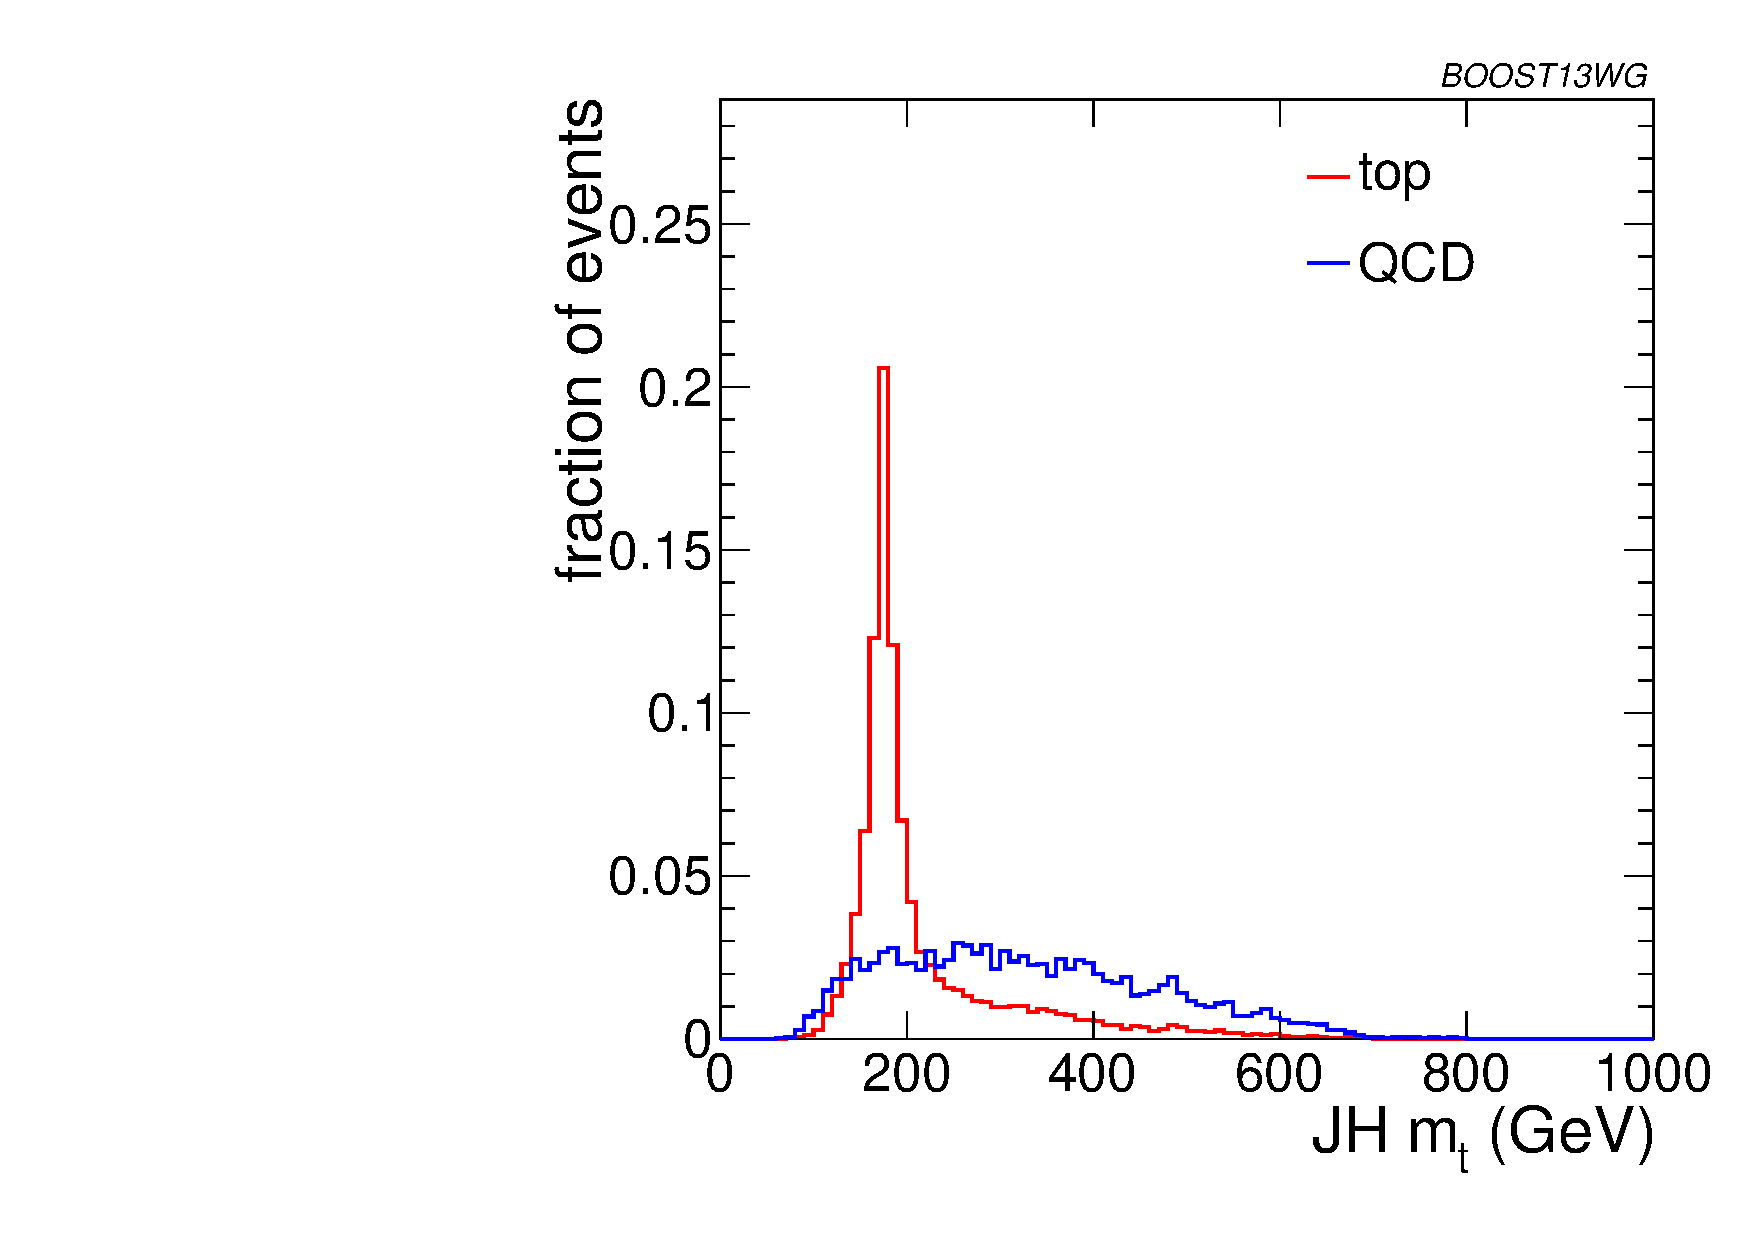
\includegraphics[width=0.48\textwidth]{./Figures/TTagging/single_variable/pT.1.5TeV.R.0.8/h_JH_mt_opt_mt.pdf}}
\subfigure[HEPTopTagger, $R=0.8$]{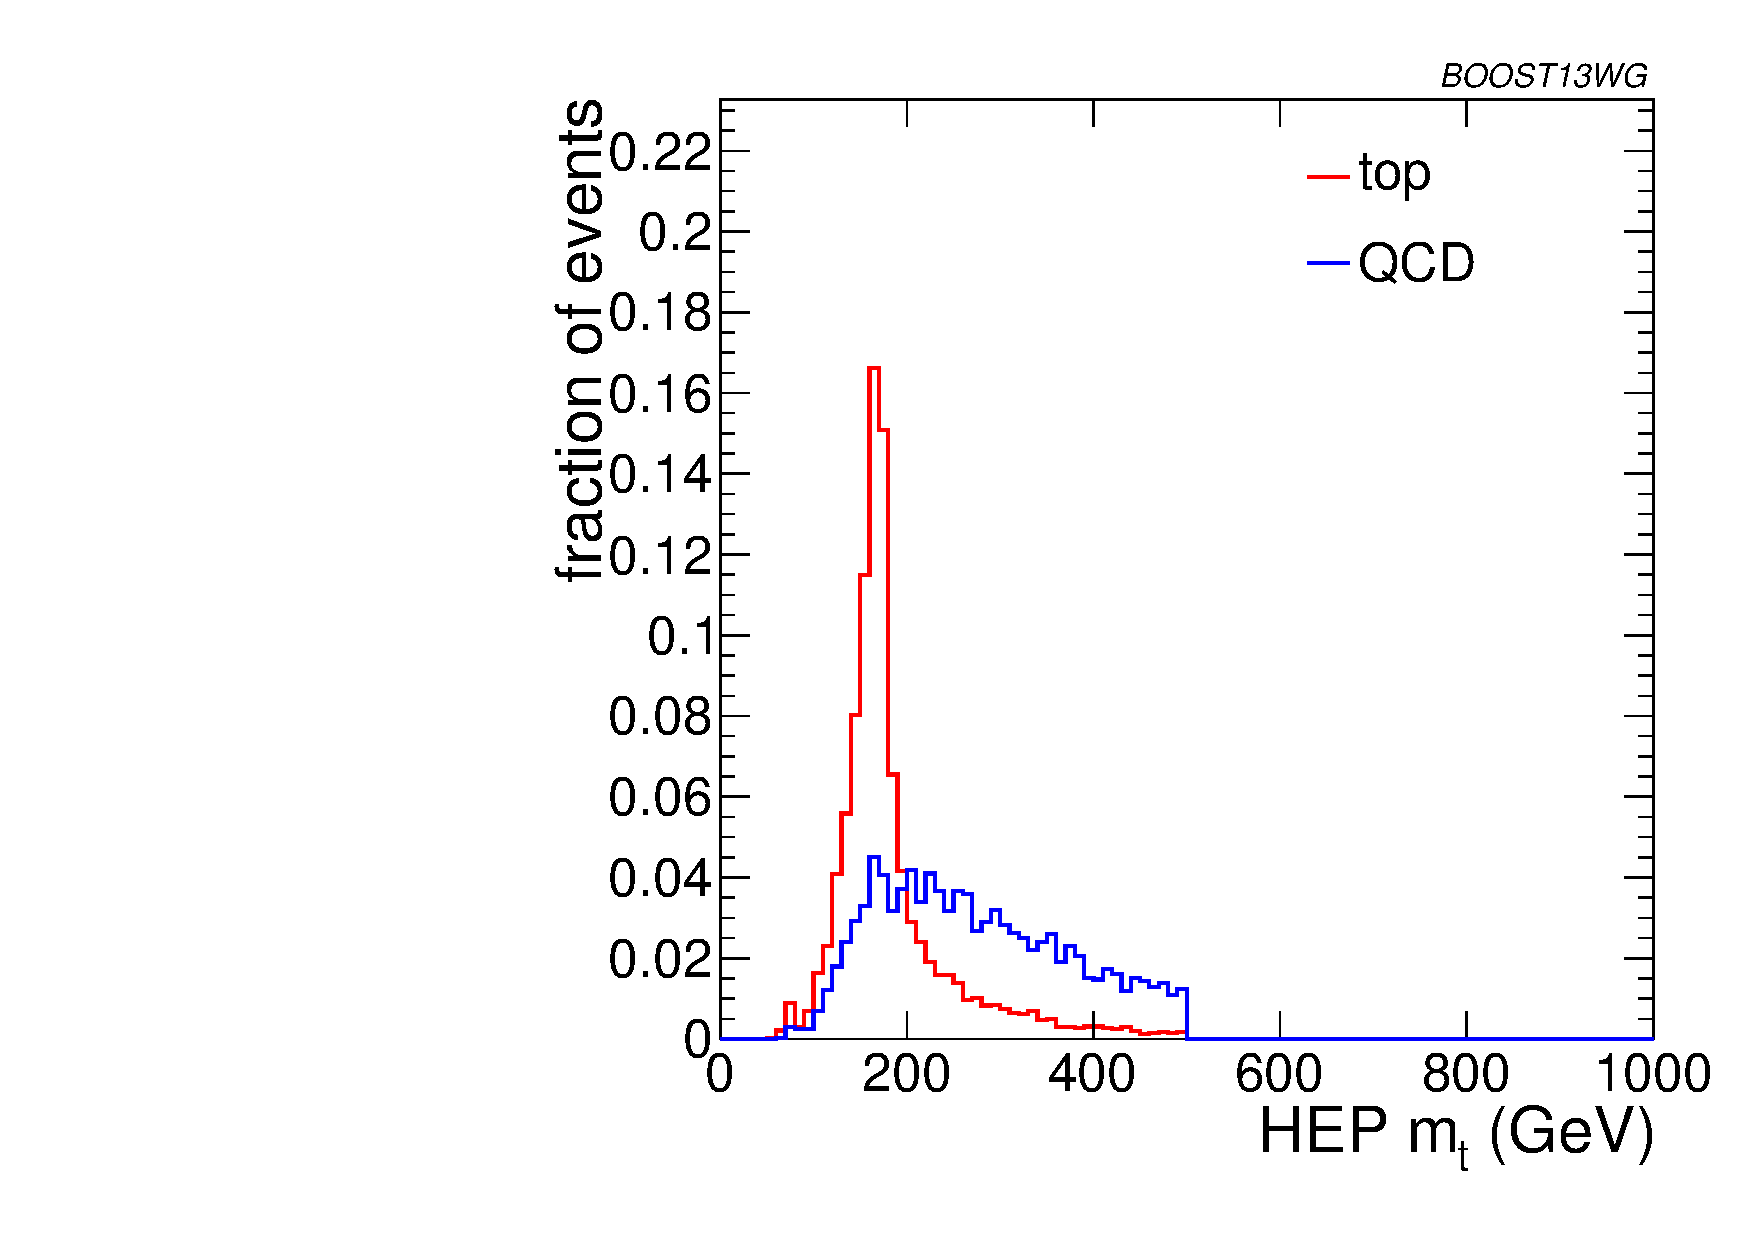
\includegraphics[width=0.48\textwidth]{./Figures/TTagging/single_variable/pT.1.5TeV.R.0.8/h_HEP_mt_opt_mt.pdf}}
\subfigure[Johns Hopkins Tagger, $R=1.2$]{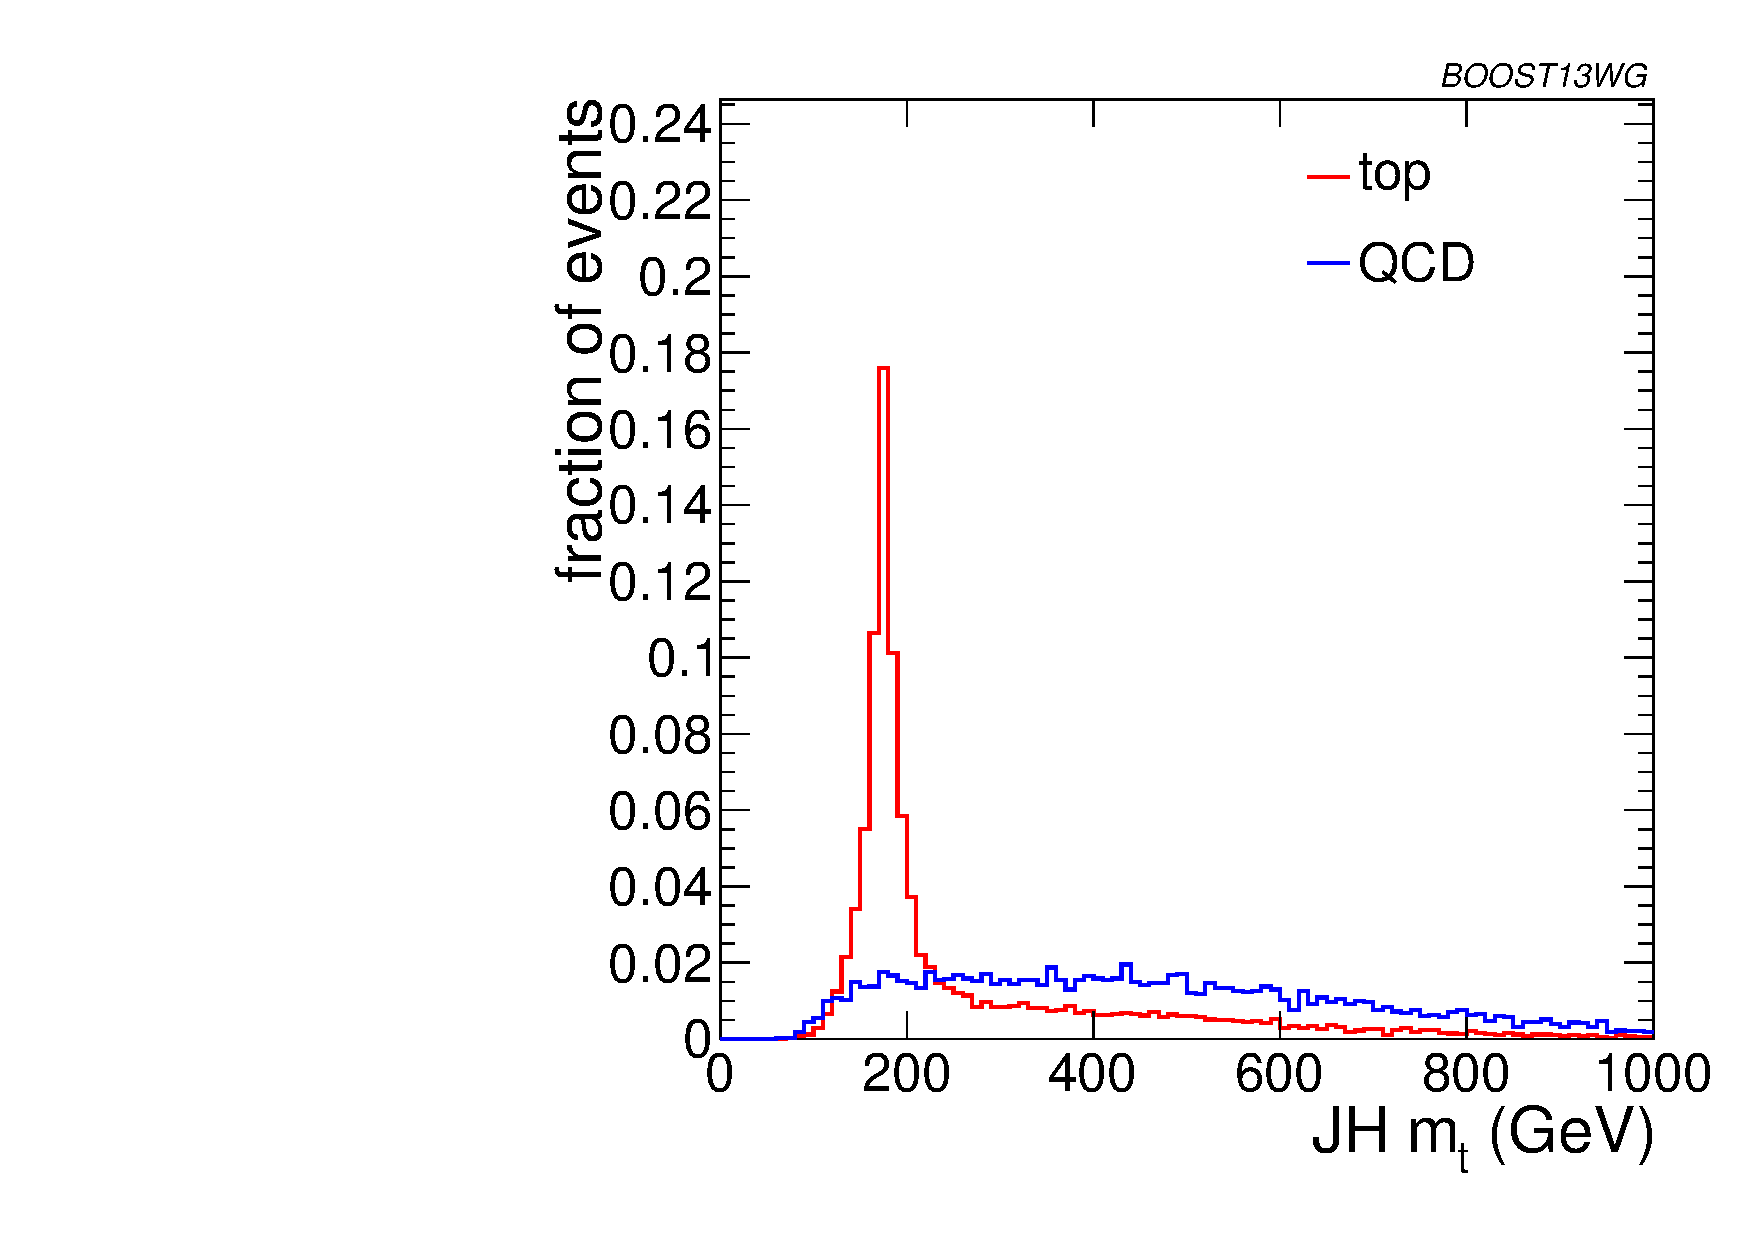
\includegraphics[width=0.48\textwidth]{./Figures/TTagging/single_variable/pT.1.5TeV.R.1.2/h_JH_mt_opt_mt.pdf}}
\subfigure[HEPTopTagger, $R=1.2$]{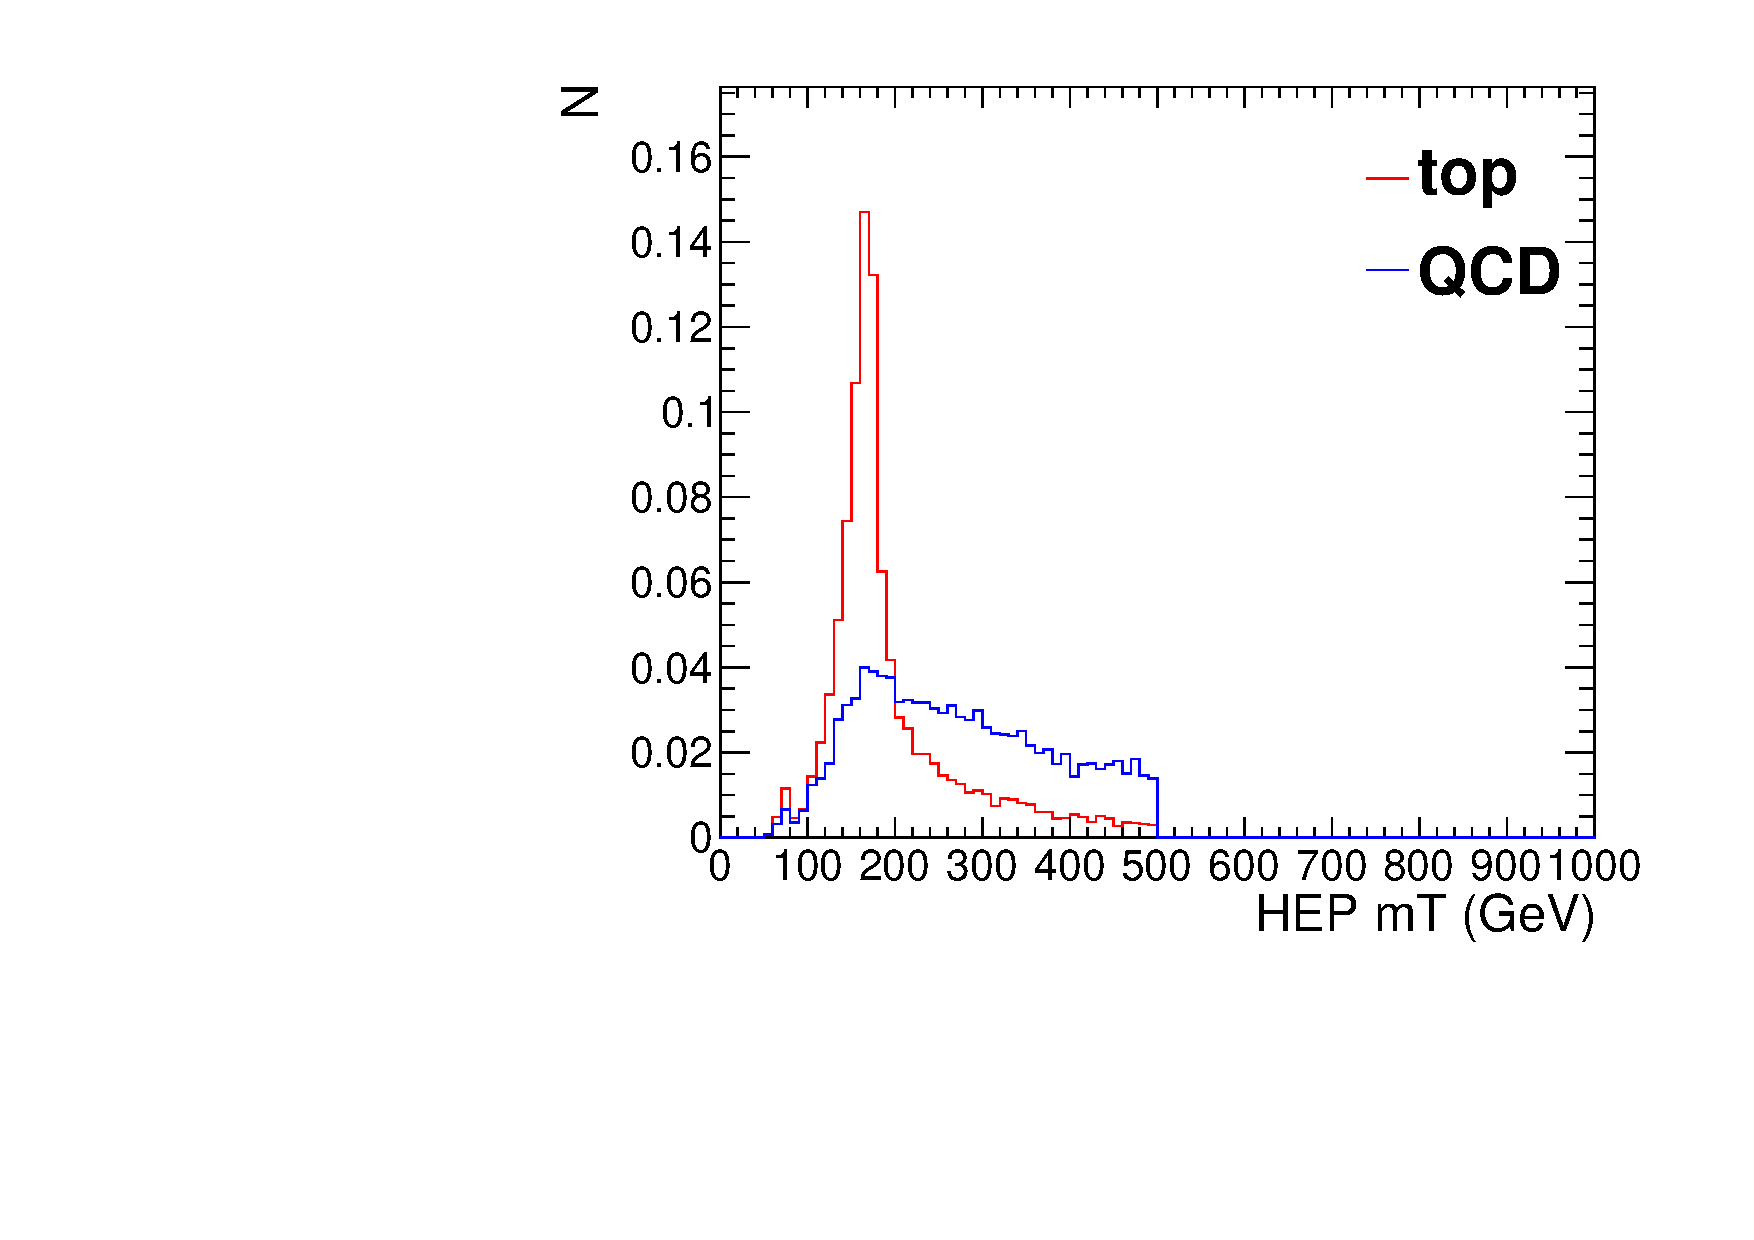
\includegraphics[width=0.48\textwidth]{./Figures/TTagging/single_variable/pT.1.5TeV.R.1.2/h_HEP_mt_opt_mt.pdf}}
\caption{Comparison of individual jet shape performance at different \pt using the anti-\kT R=0.8 algorithm, $p_{\rm T}=1.5-1.6$ TeV. Each histogram is shown for the working point optimized for best performance with $m_t$ at signal efficiency 0.3.}
\label{fig:topmass_histogram_HEP_JH}
\end{center}
\end{figure*}

\begin{figure*}
\begin{center}
\subfigure[Johns Hopkins Tagger, $R=0.4$]{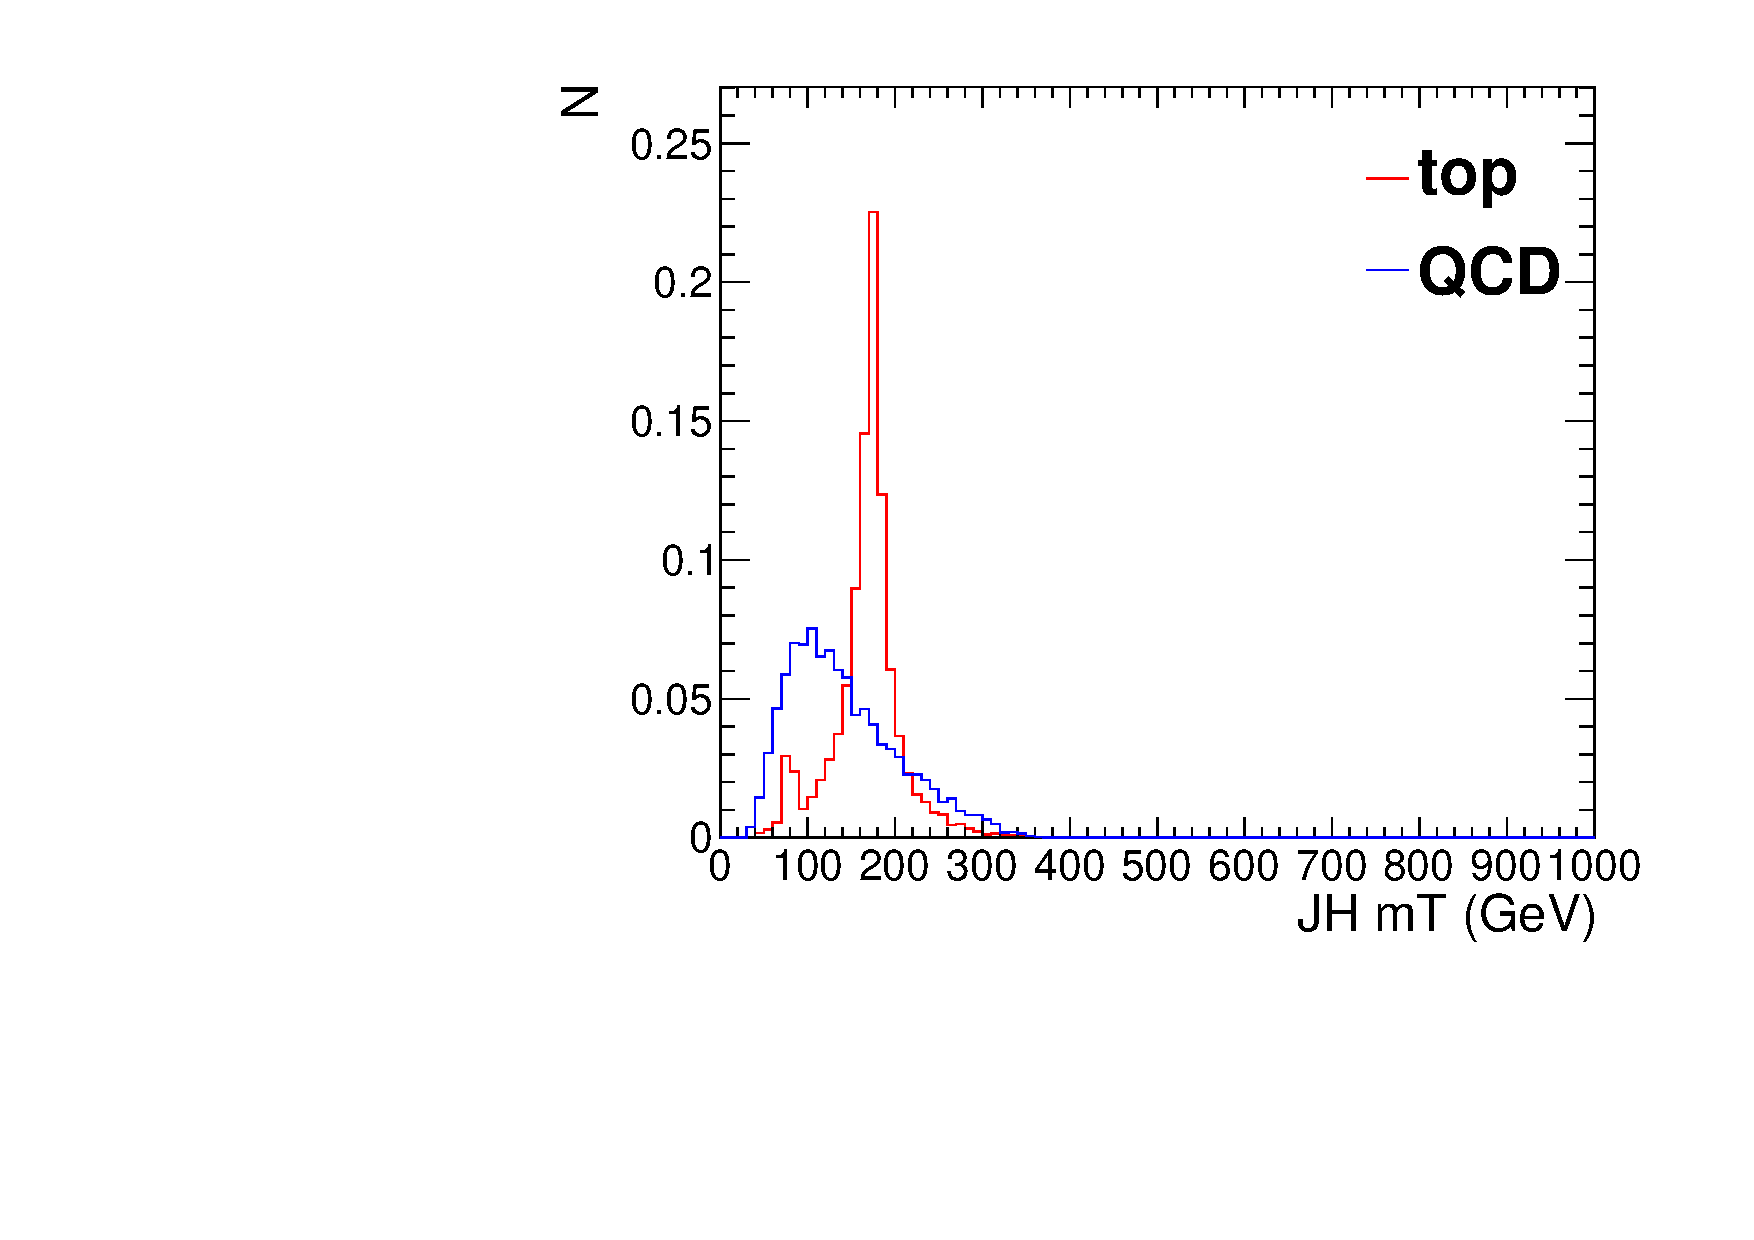
\includegraphics[width=0.48\textwidth]{./Figures/TTagging/single_variable/pT.1.5TeV.R.0.4/h_JH_mt_opt_all.pdf}}
\subfigure[HEPTopTagger, $R=0.4$]{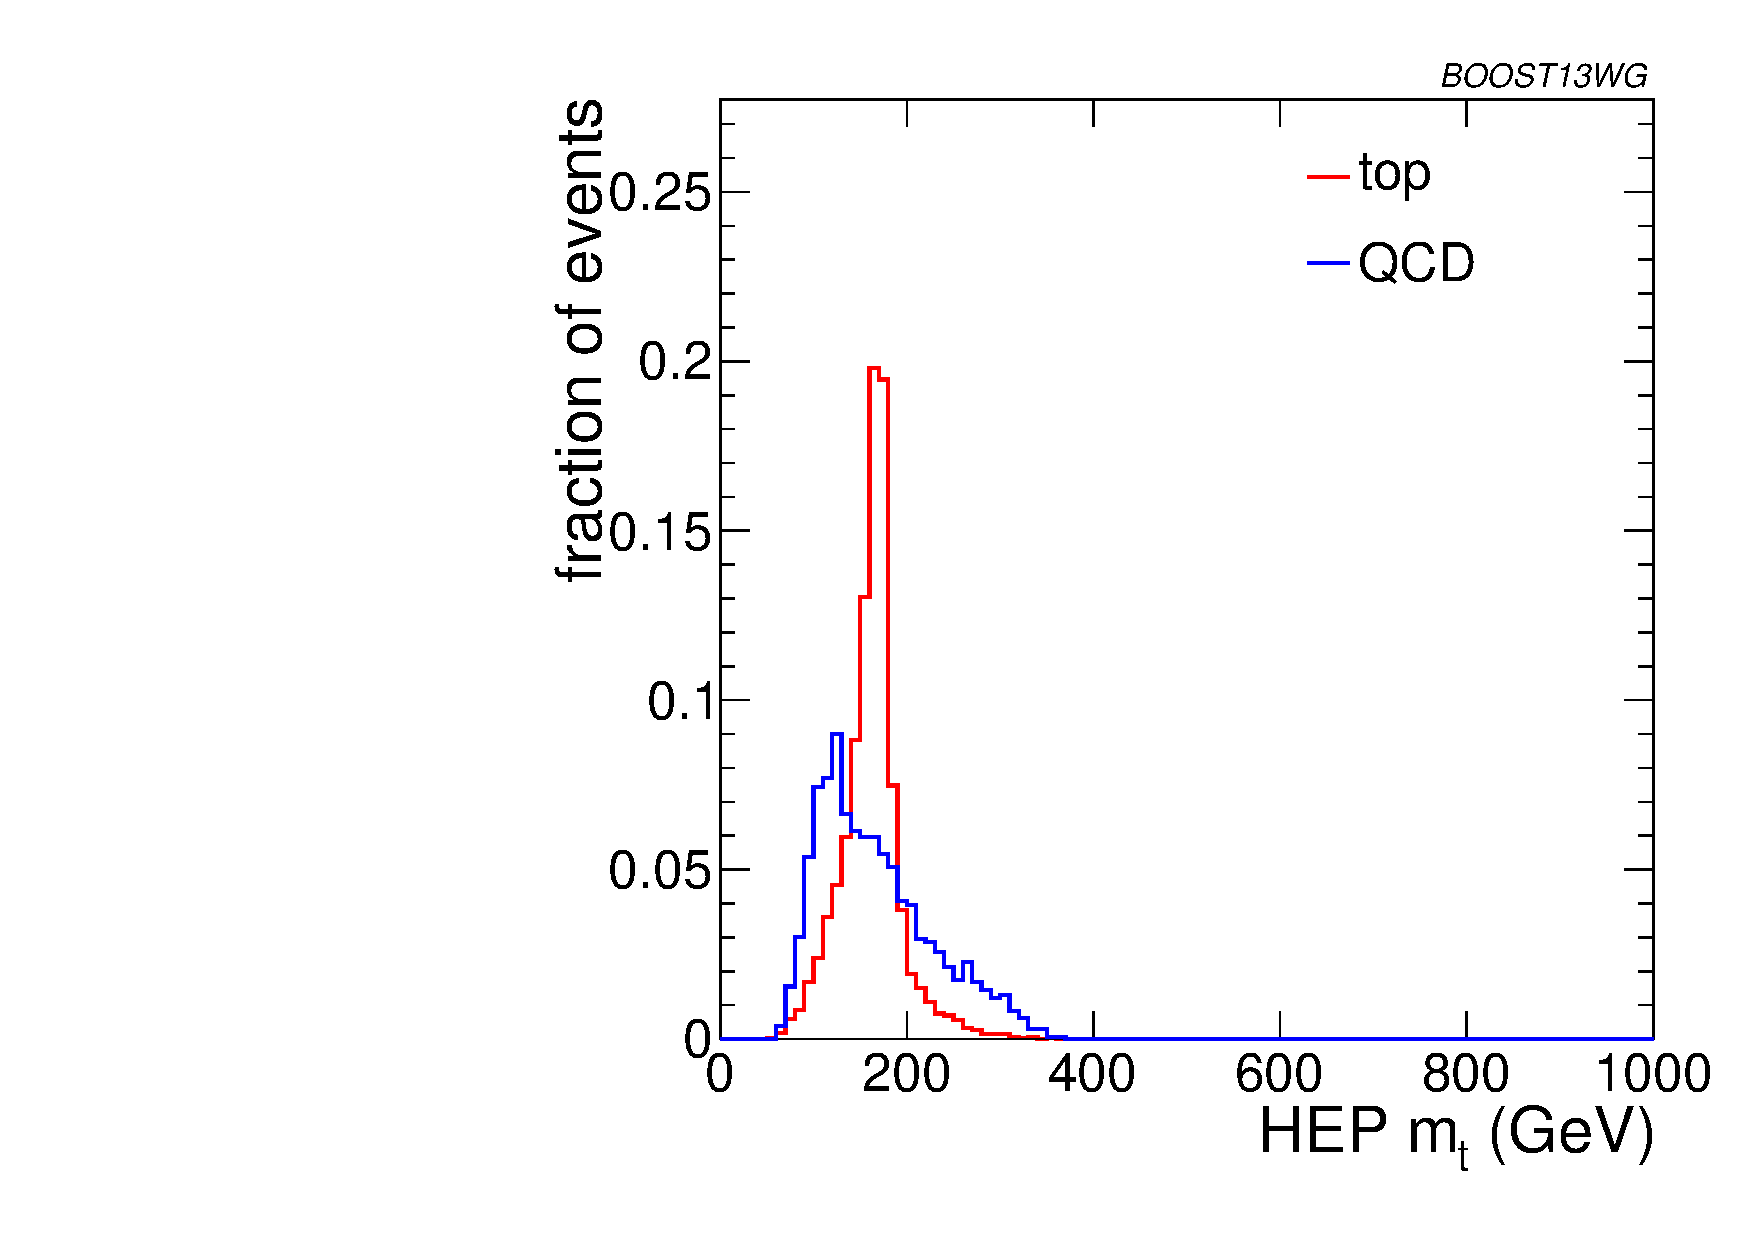
\includegraphics[width=0.48\textwidth]{./Figures/TTagging/single_variable/pT.1.5TeV.R.0.4/h_HEP_mt_opt_all.pdf}}
\subfigure[Johns Hopkins Tagger, $R=0.8$]{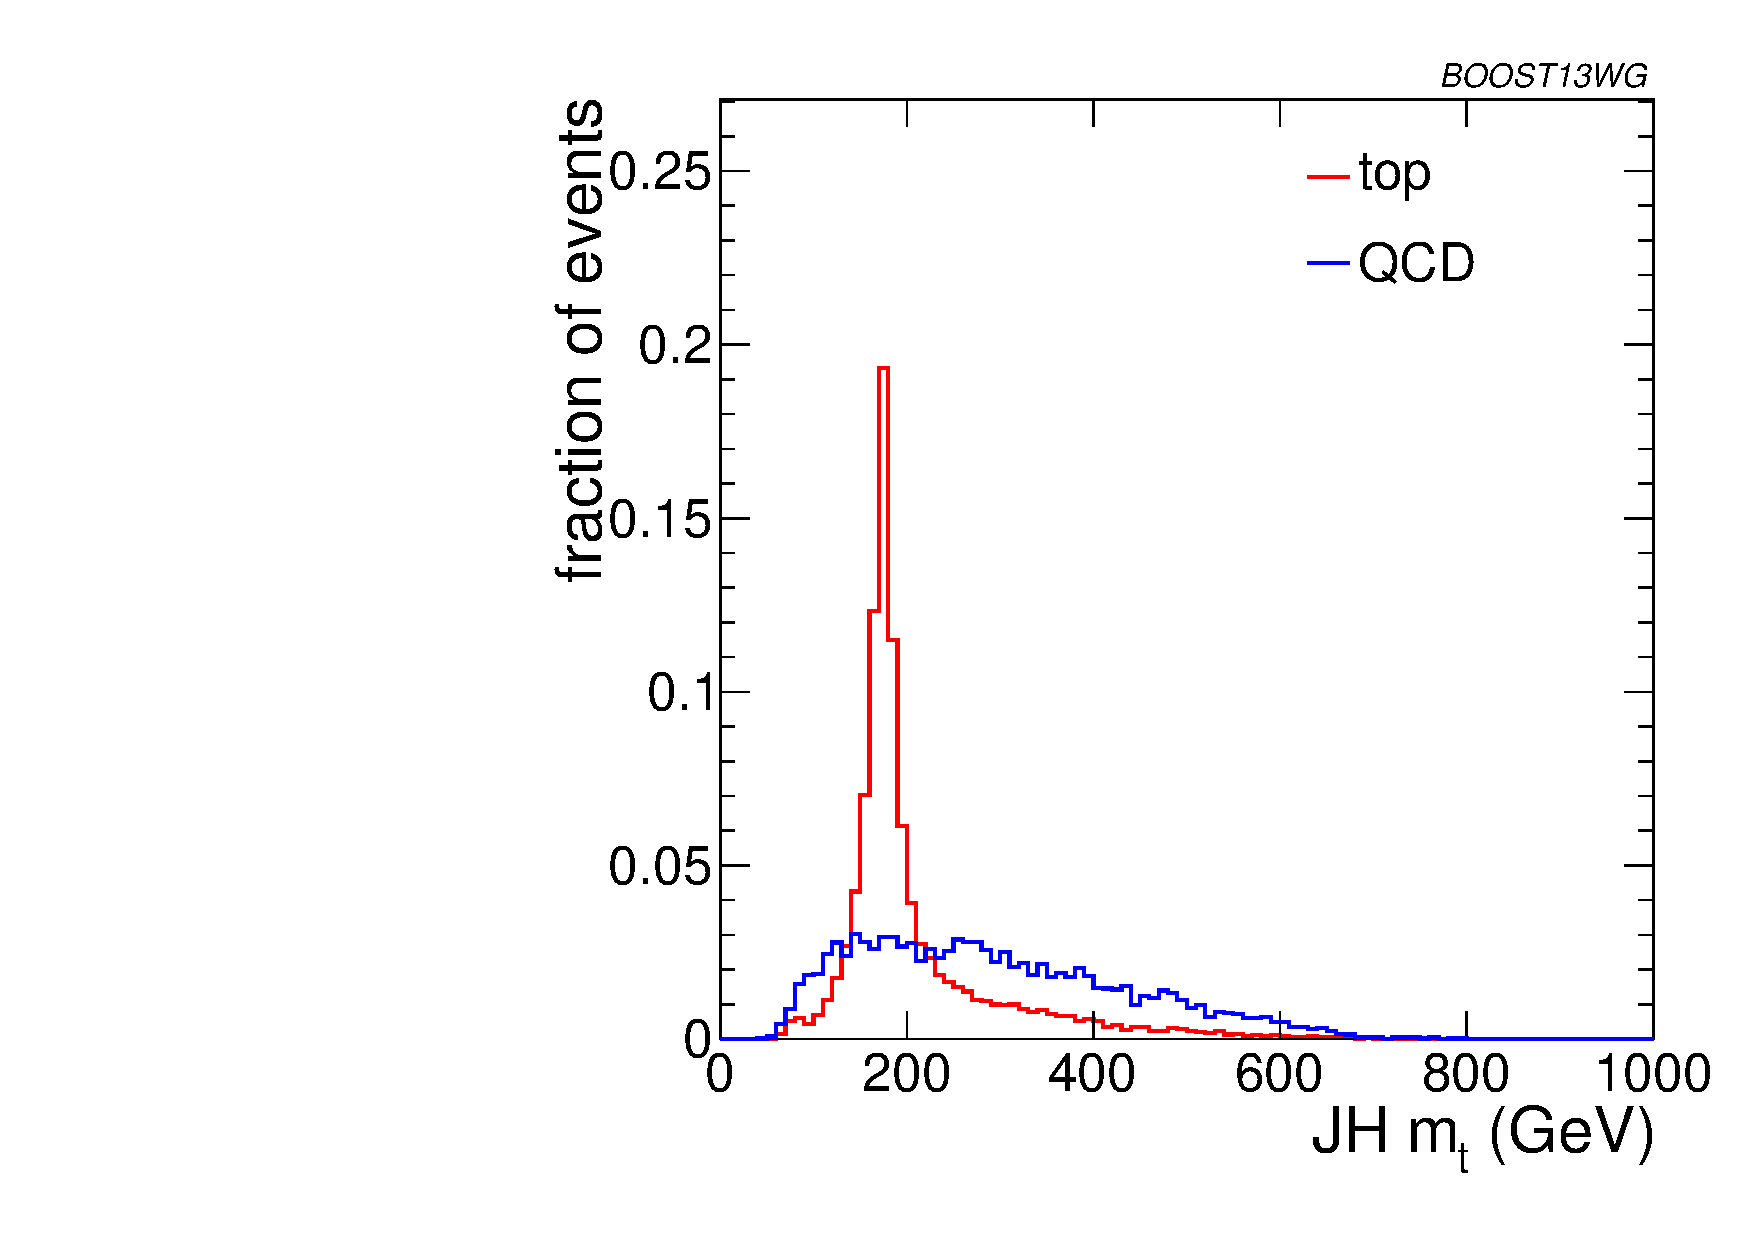
\includegraphics[width=0.48\textwidth]{./Figures/TTagging/single_variable/pT.1.5TeV.R.0.8/h_JH_mt_opt_all.pdf}}
\subfigure[HEPTopTagger, $R=0.8$]{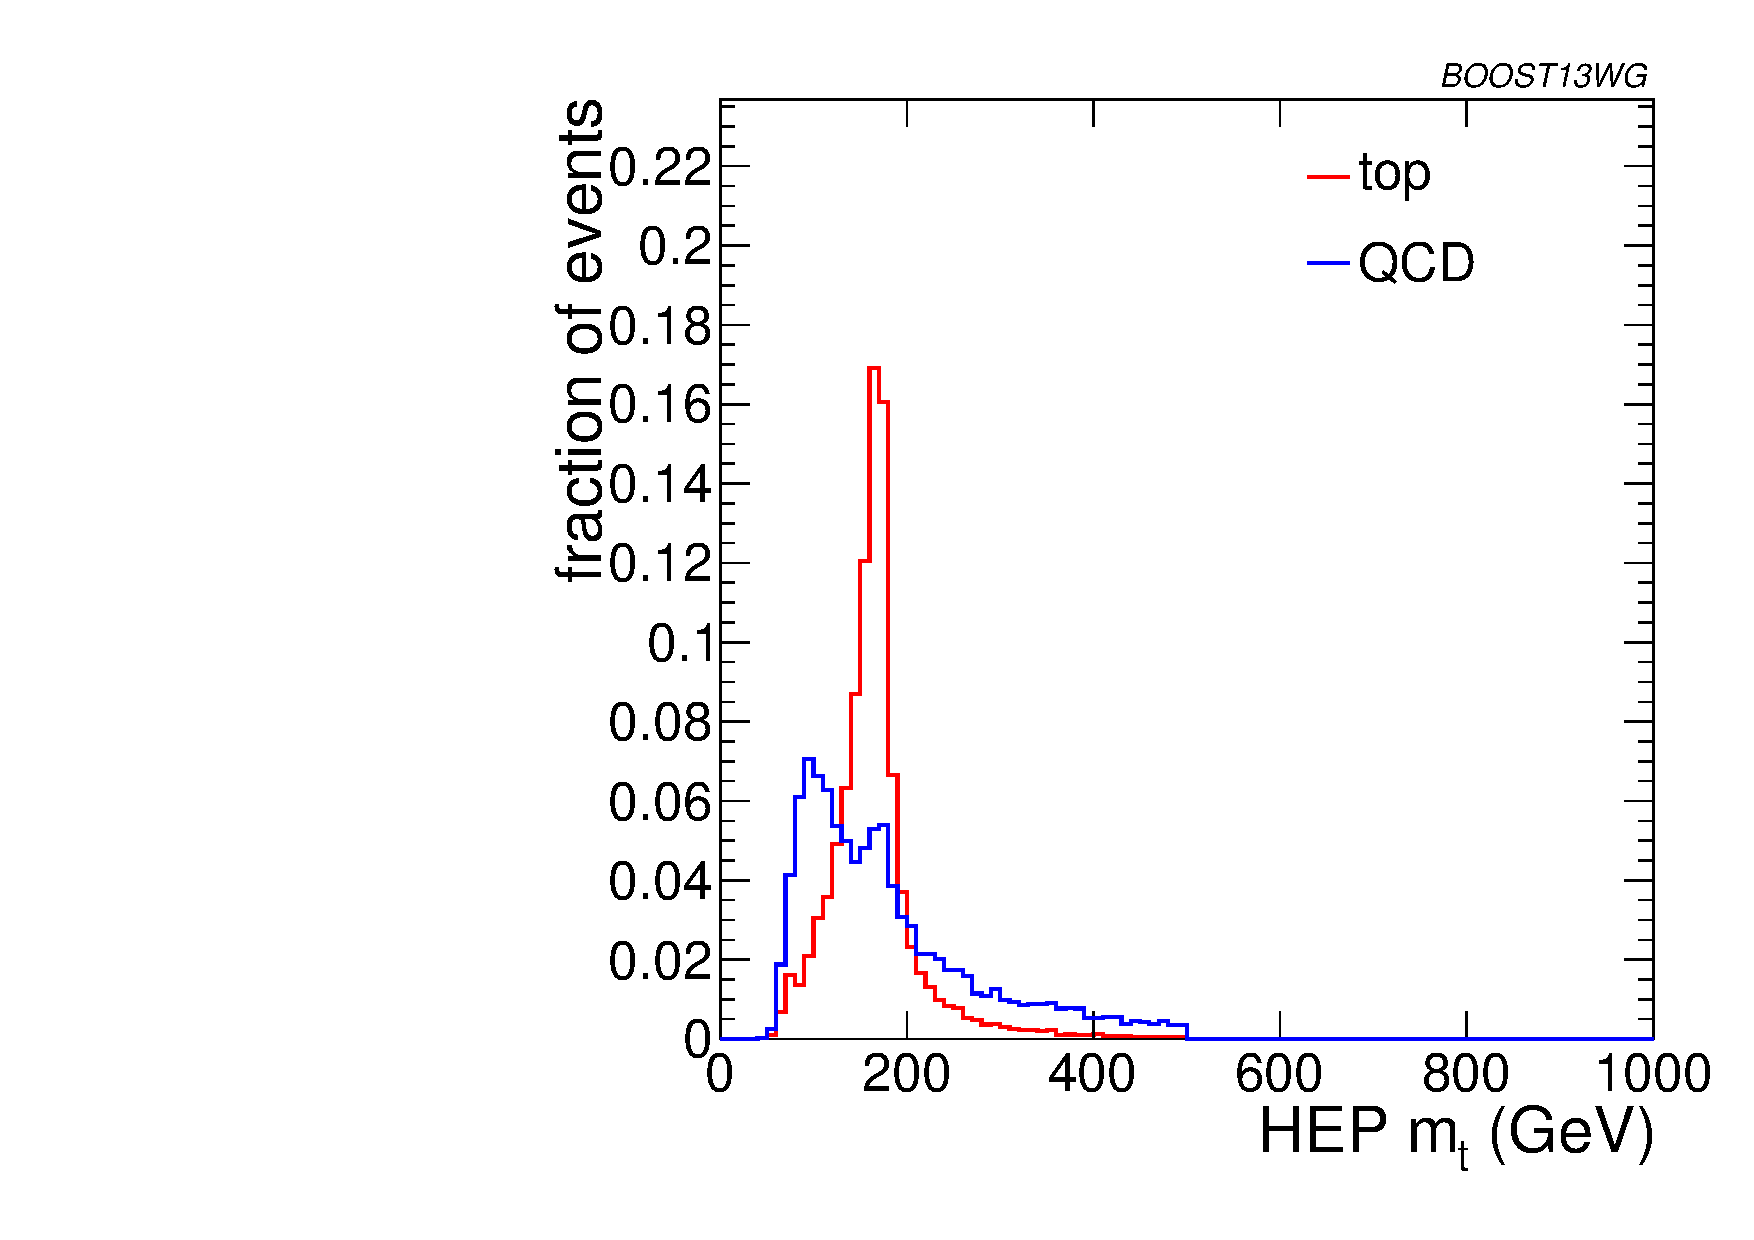
\includegraphics[width=0.48\textwidth]{./Figures/TTagging/single_variable/pT.1.5TeV.R.0.8/h_HEP_mt_opt_all.pdf}}
\subfigure[Johns Hopkins Tagger, $R=1.2$]{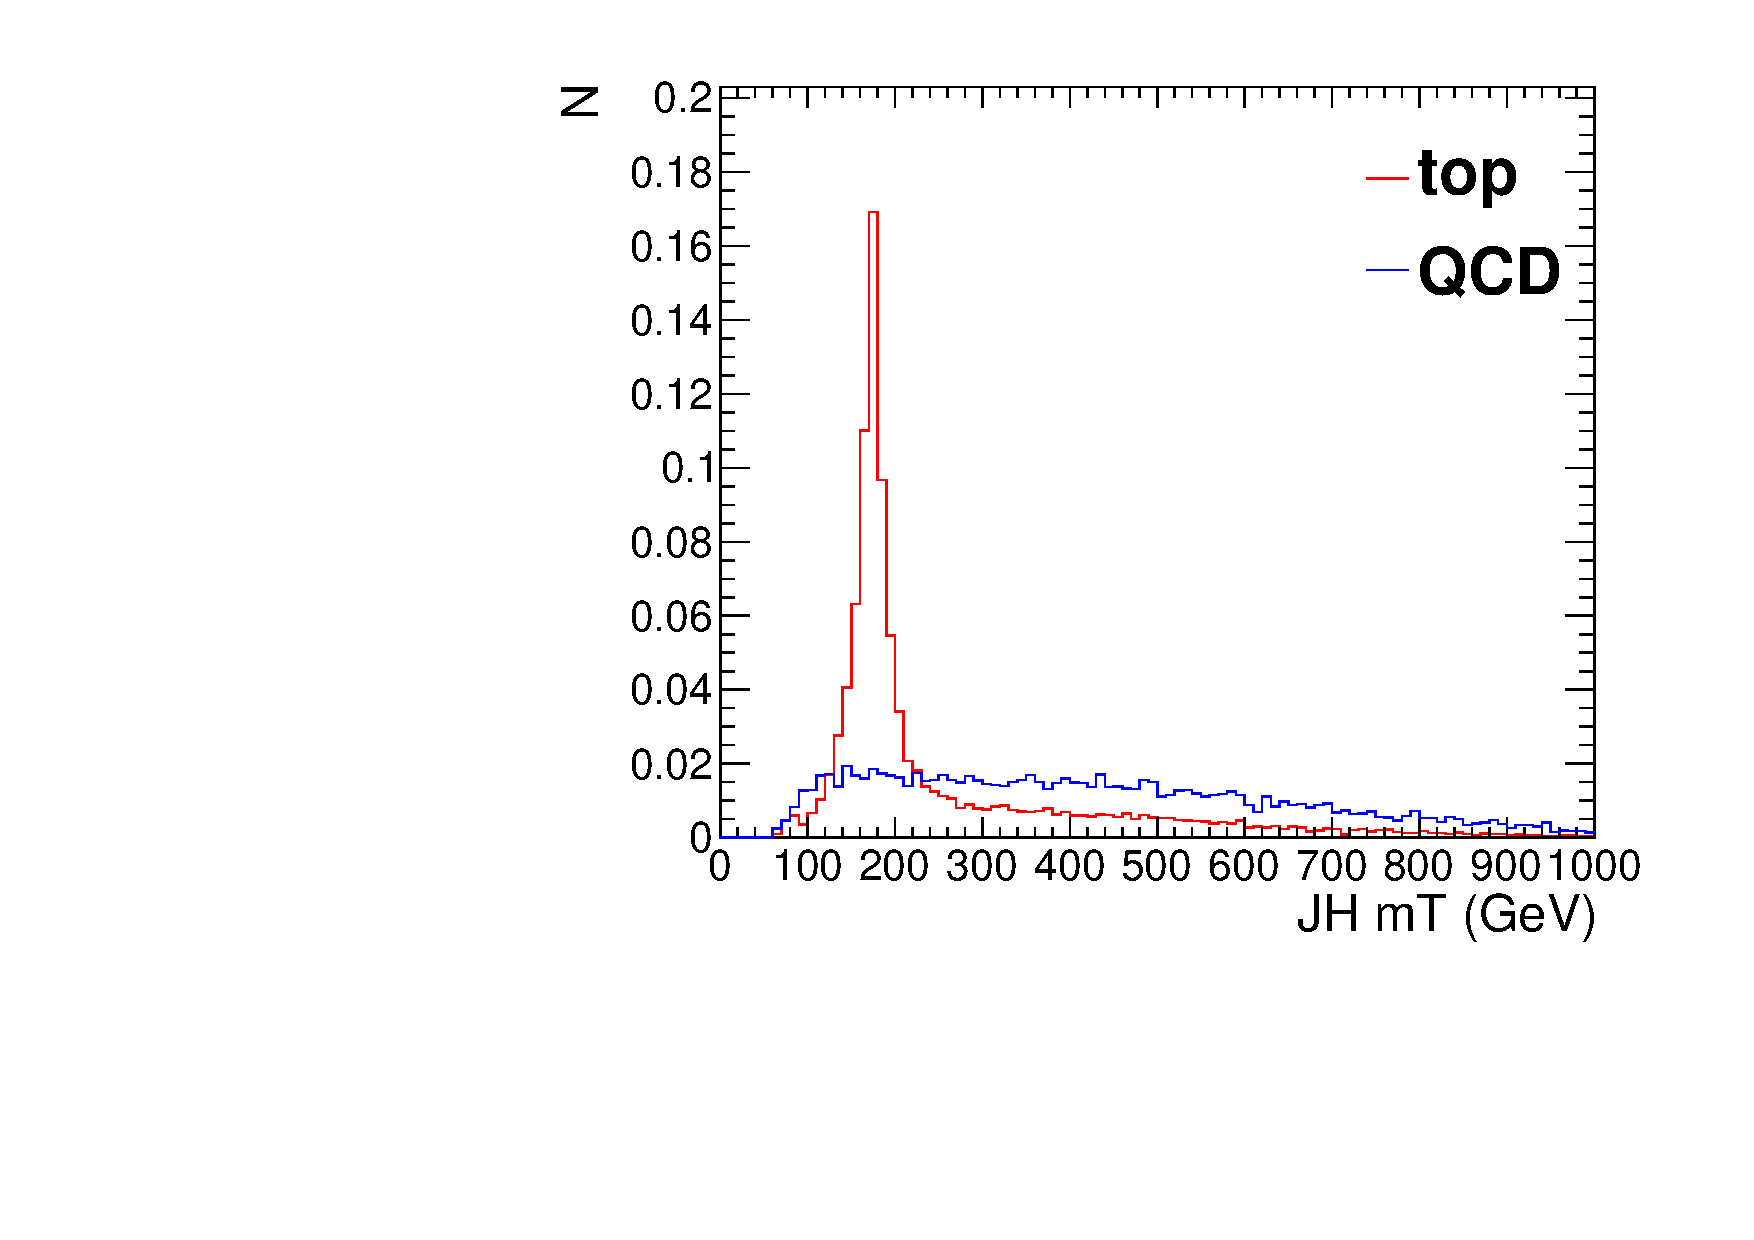
\includegraphics[width=0.48\textwidth]{./Figures/TTagging/single_variable/pT.1.5TeV.R.1.2/h_JH_mt_opt_all.pdf}}
\subfigure[HEPTopTagger, $R=1.2$]{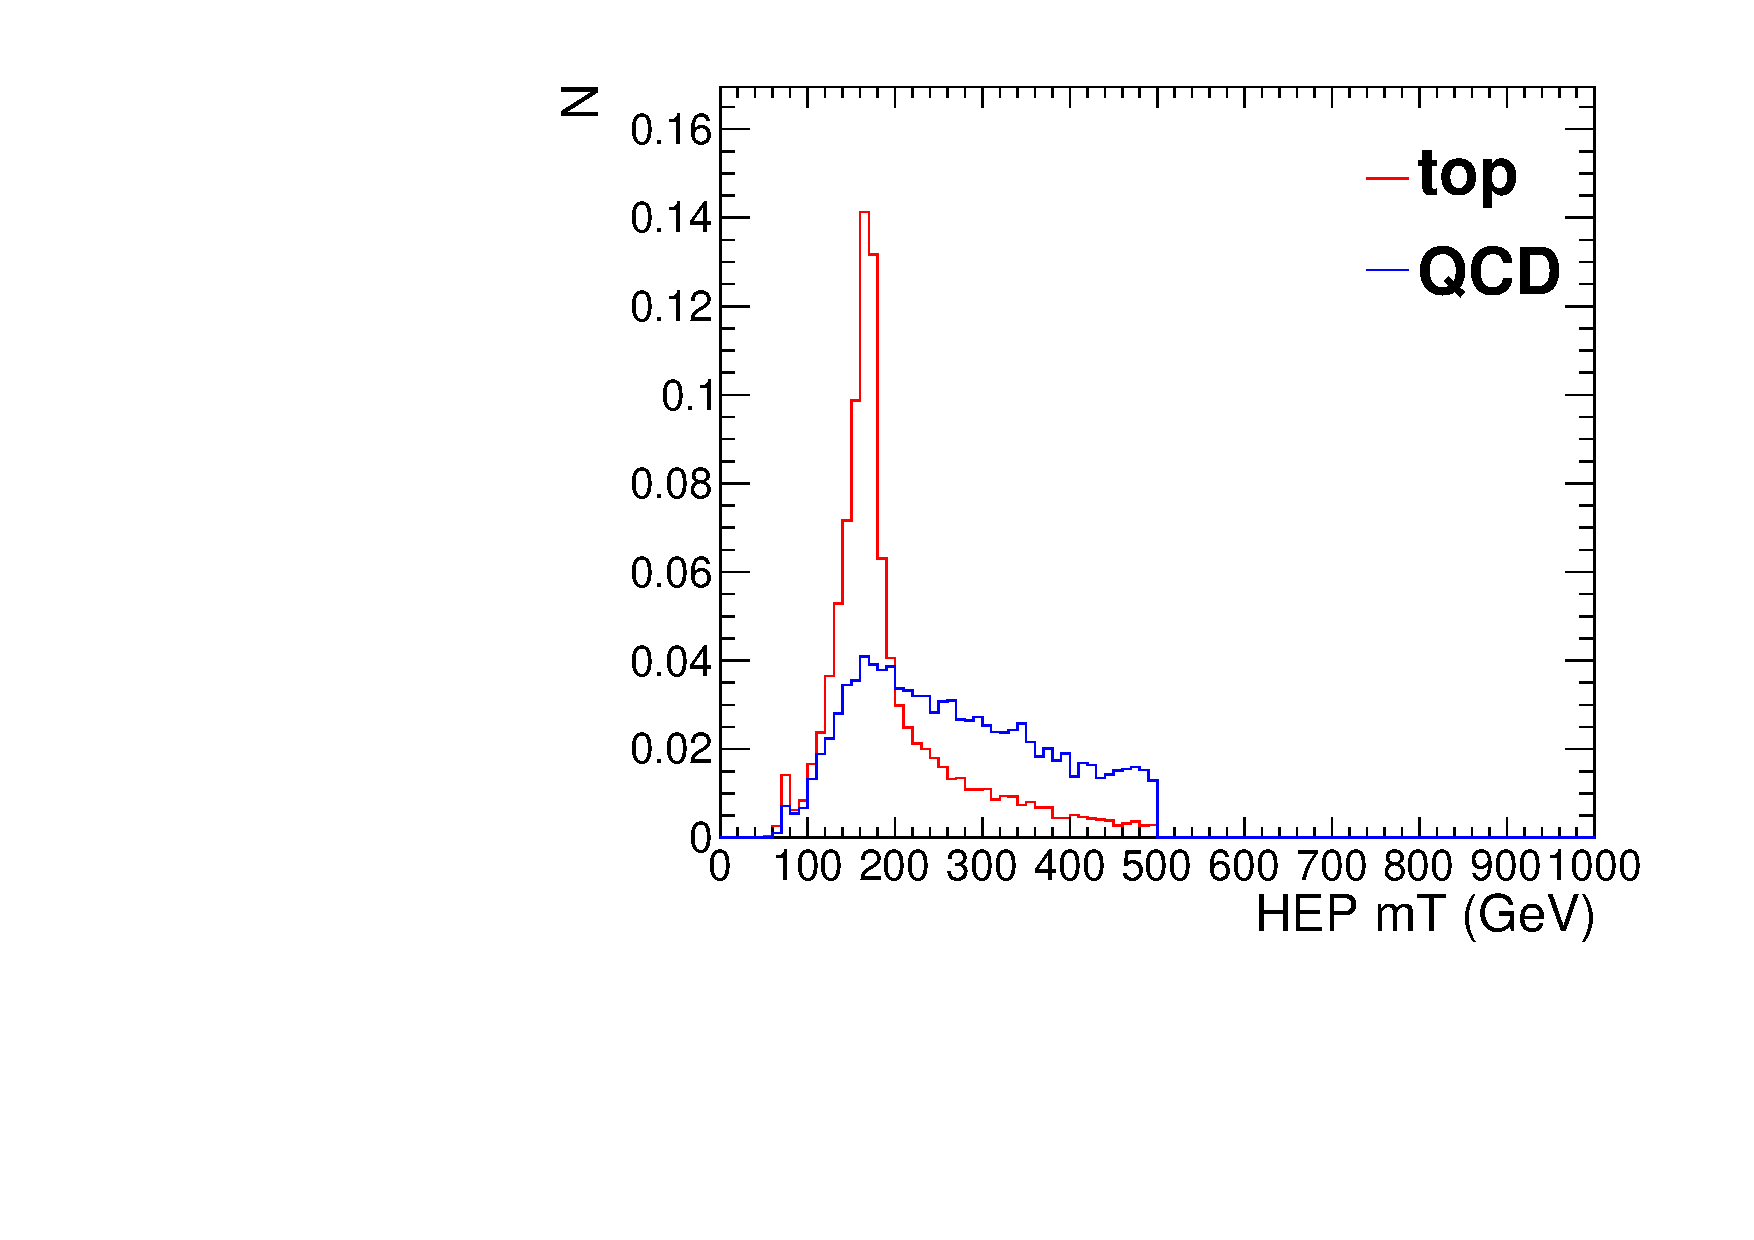
\includegraphics[width=0.48\textwidth]{./Figures/TTagging/single_variable/pT.1.5TeV.R.1.2/h_HEP_mt_opt_all.pdf}}
\caption{Comparison of individual jet shape performance at different \pt using the anti-\kT R=0.8 algorithm, $p_{\rm T}=1.5-1.6$ TeV. Each histogram is shown for the working point optimized for best performance of the tagger at signal efficiency 0.3.}
\label{fig:topmass_histogram_optall_HEP_JH}
\end{center}
\end{figure*}

\begin{figure*}
\begin{center}
\subfigure[Johns Hopkins Tagger, $R=0.4$]{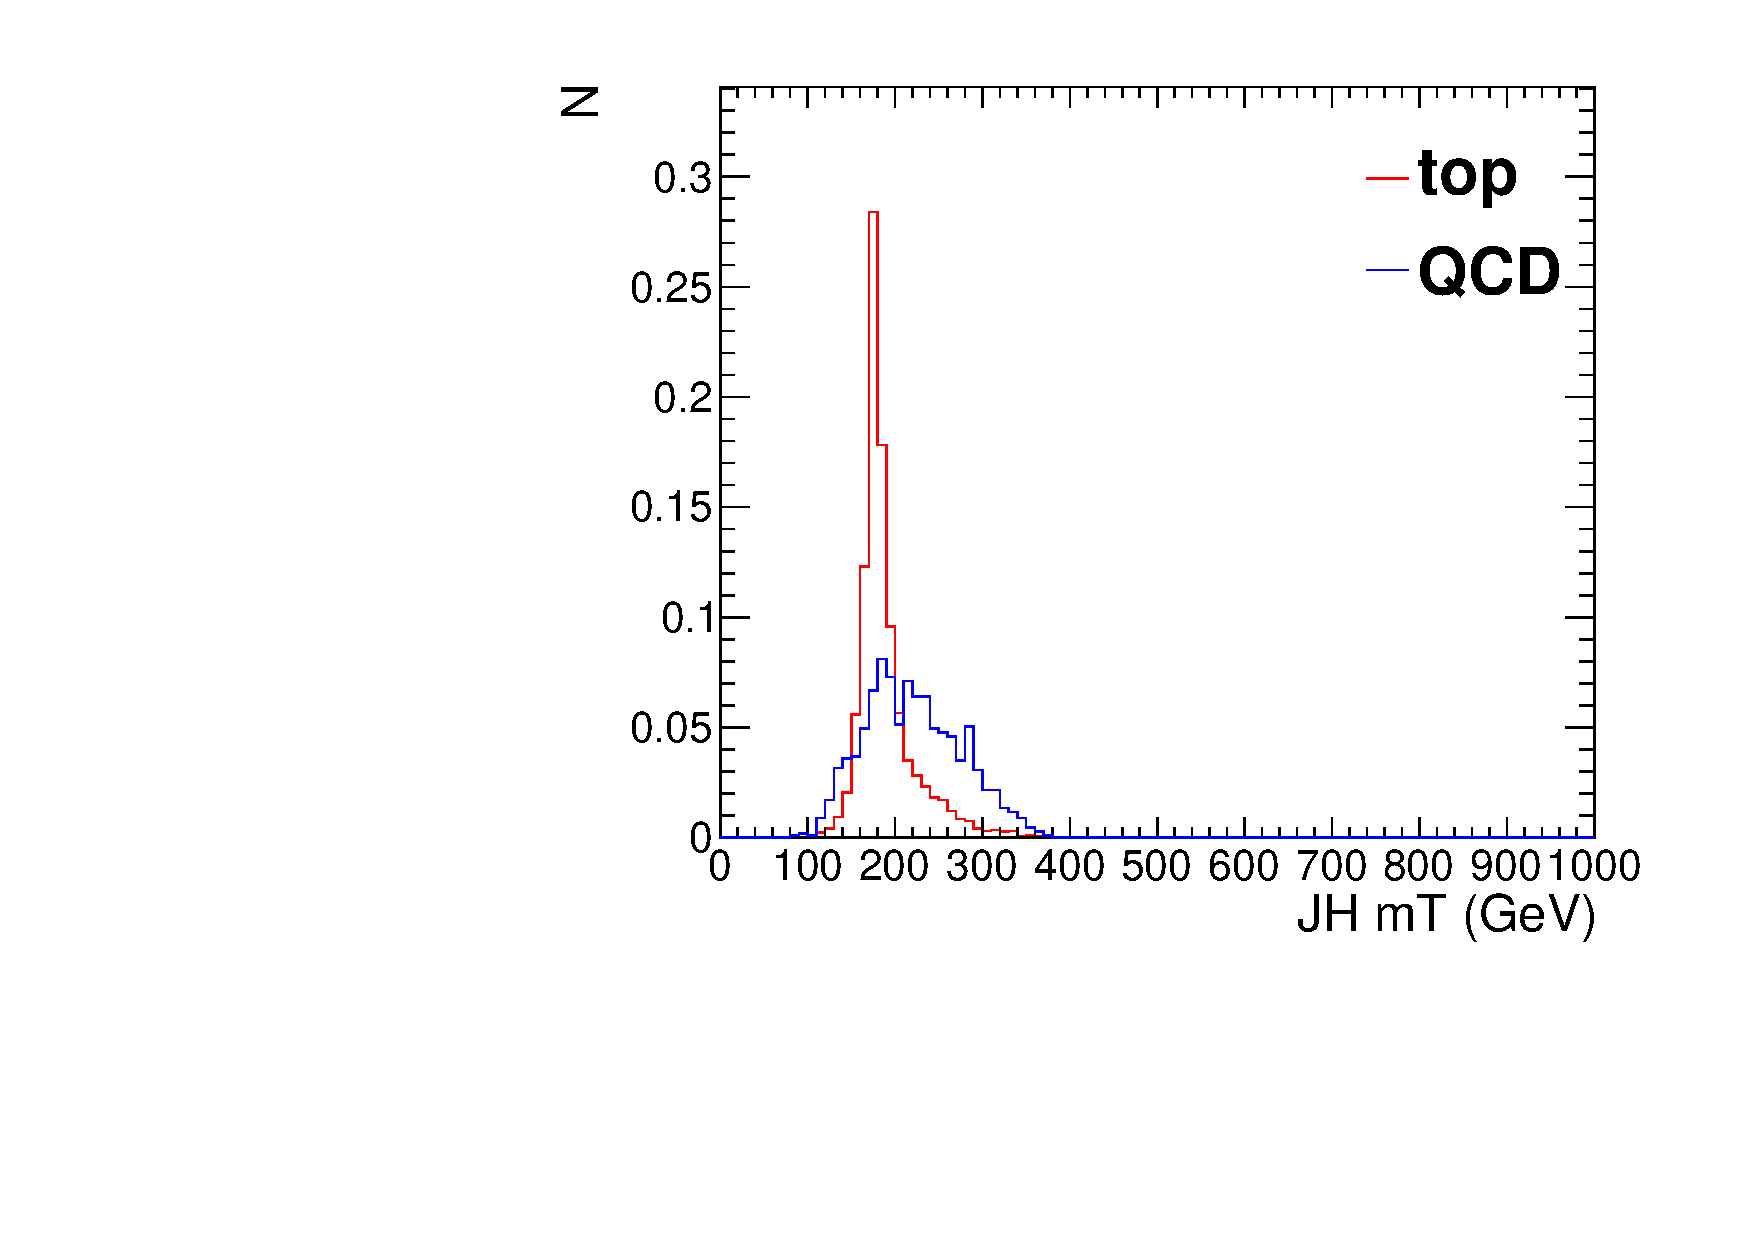
\includegraphics[width=0.48\textwidth]{./Figures/TTagging/single_variable/pT.1.5TeV.R.0.4/h_JH_mt_opt_all_once.pdf}}
\subfigure[HEPTopTagger, $R=0.4$]{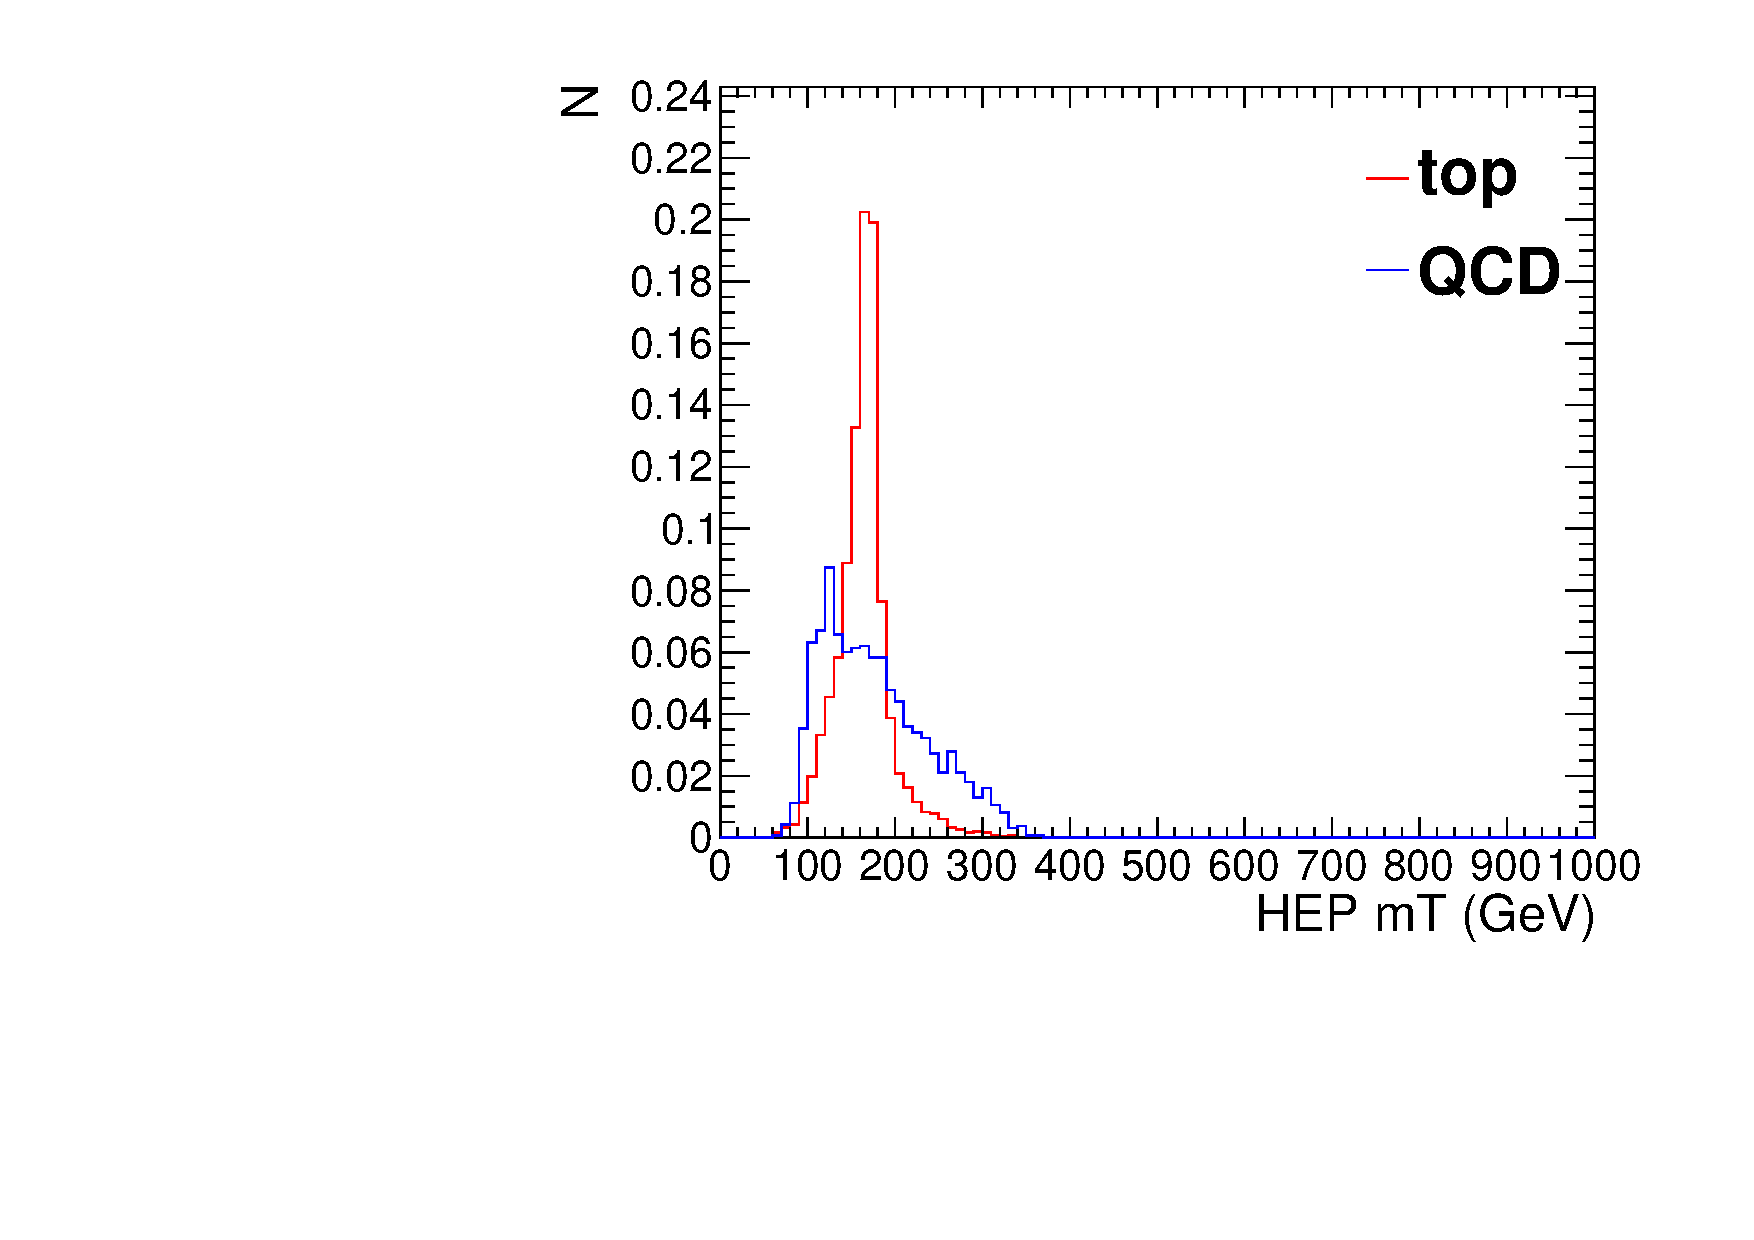
\includegraphics[width=0.48\textwidth]{./Figures/TTagging/single_variable/pT.1.5TeV.R.0.4/h_HEP_mt_opt_all_once.pdf}}
\subfigure[Johns Hopkins Tagger, $R=0.8$]{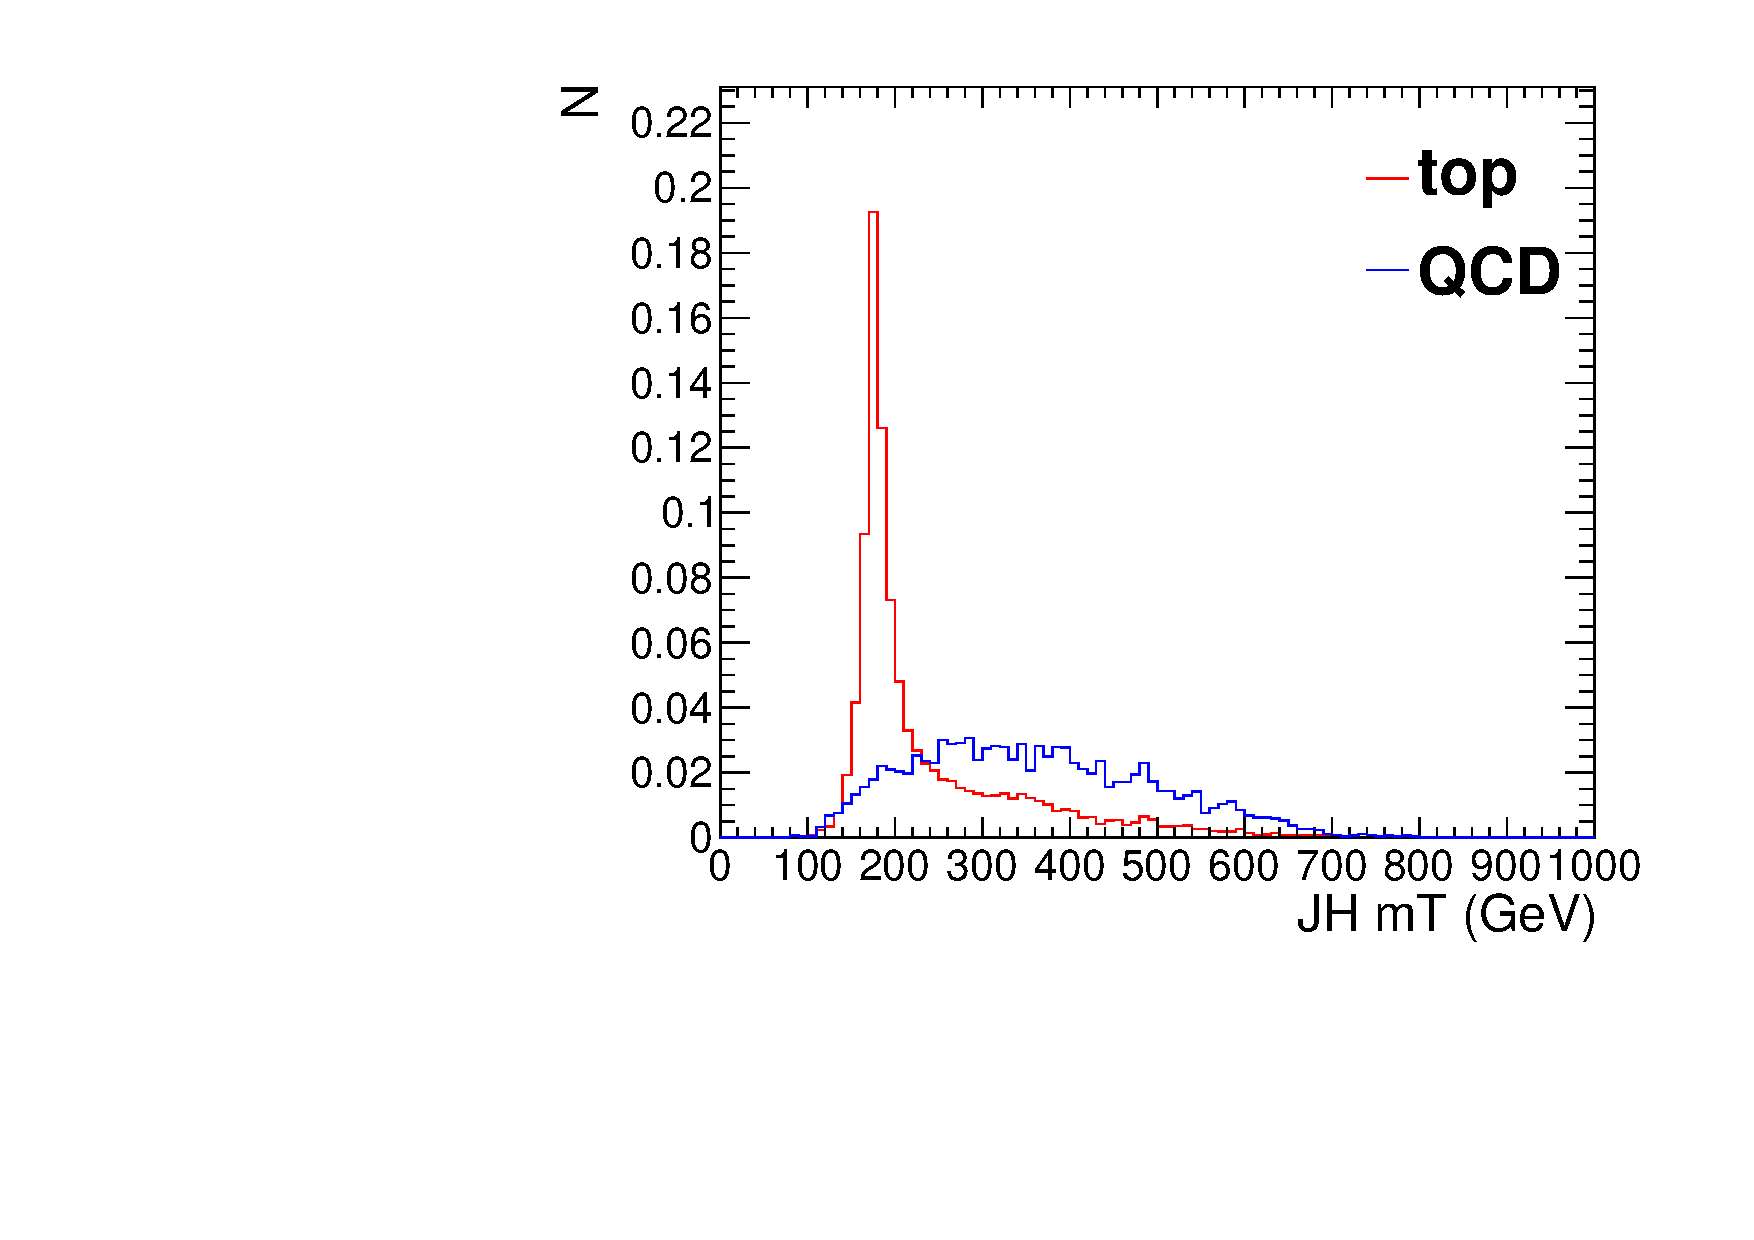
\includegraphics[width=0.48\textwidth]{./Figures/TTagging/single_variable/pT.1.5TeV.R.0.8/h_JH_mt_opt_all_once.pdf}}
\subfigure[HEPTopTagger, $R=0.8$]{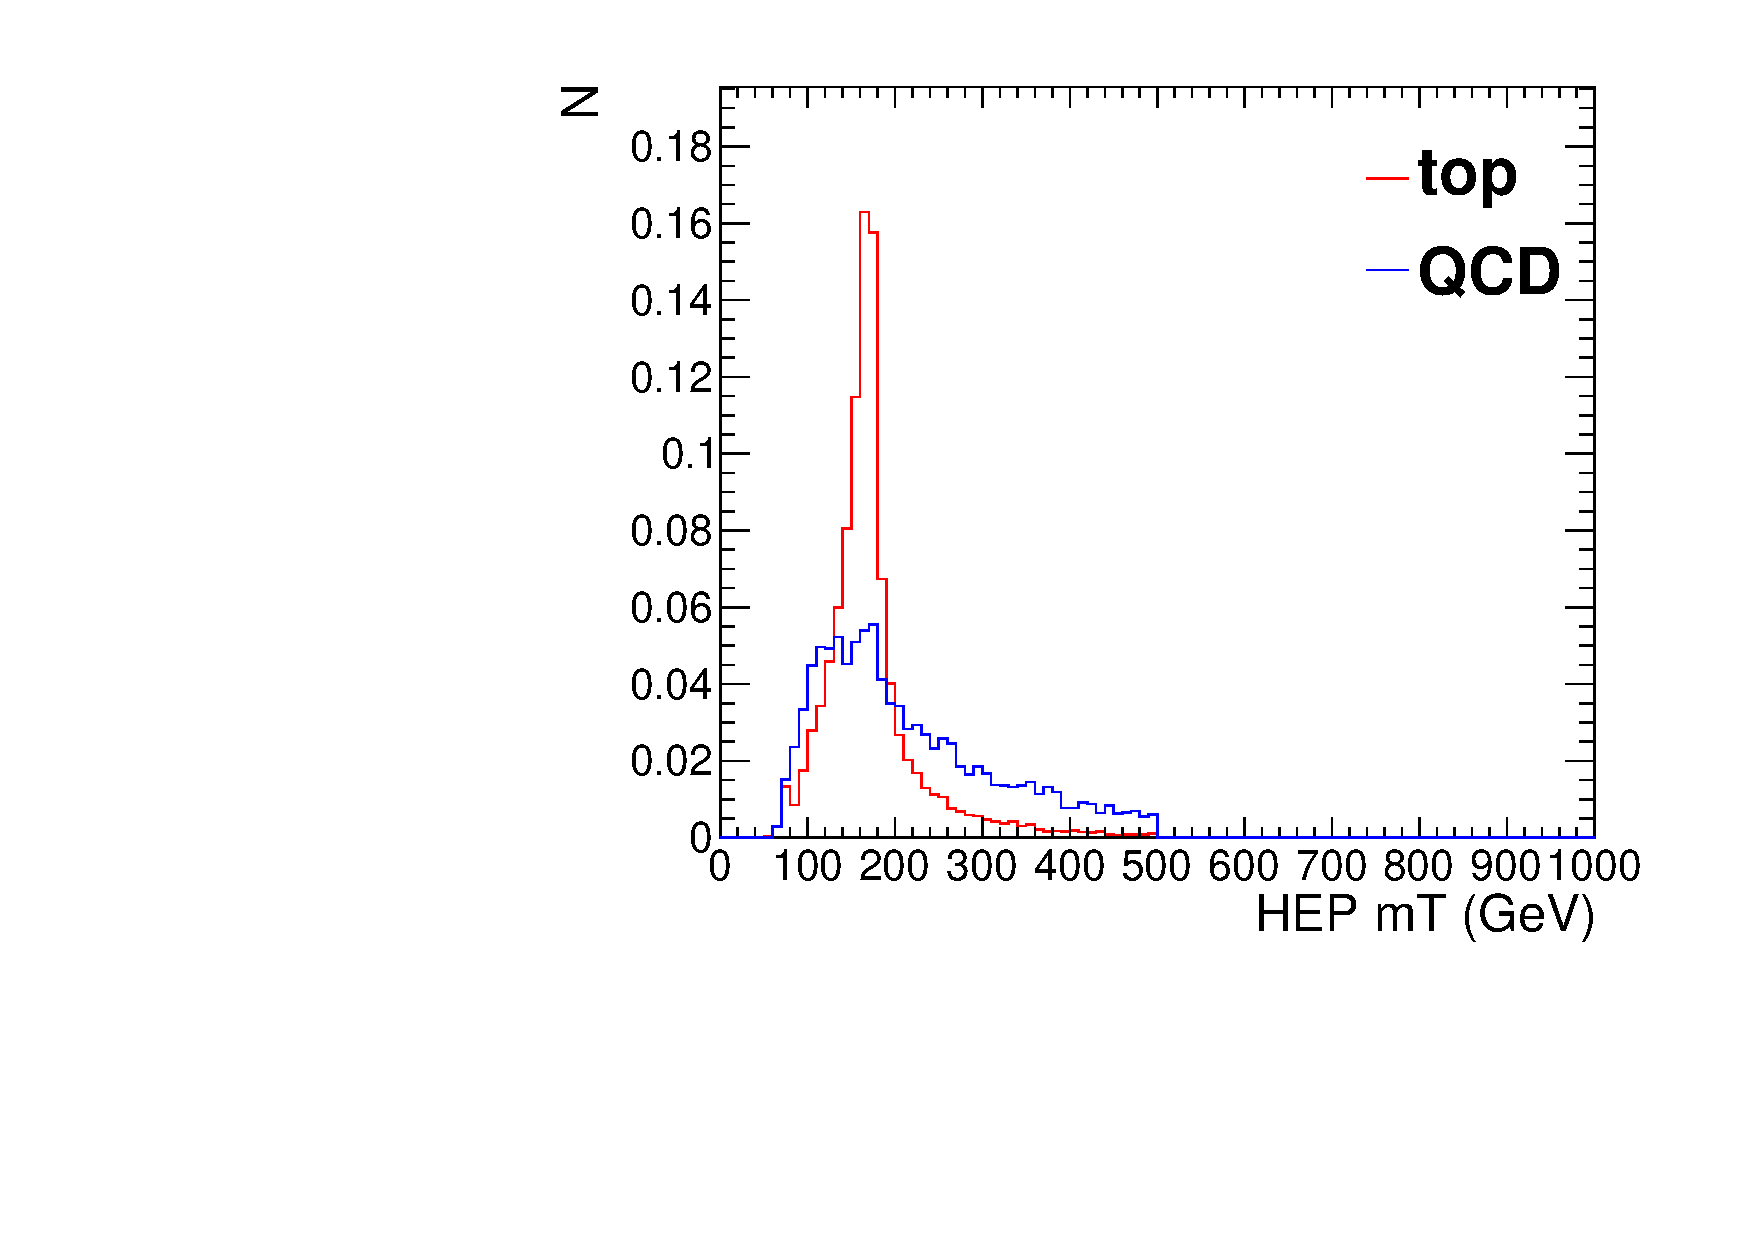
\includegraphics[width=0.48\textwidth]{./Figures/TTagging/single_variable/pT.1.5TeV.R.0.8/h_HEP_mt_opt_all_once.pdf}}
\subfigure[Johns Hopkins Tagger, $R=1.2$]{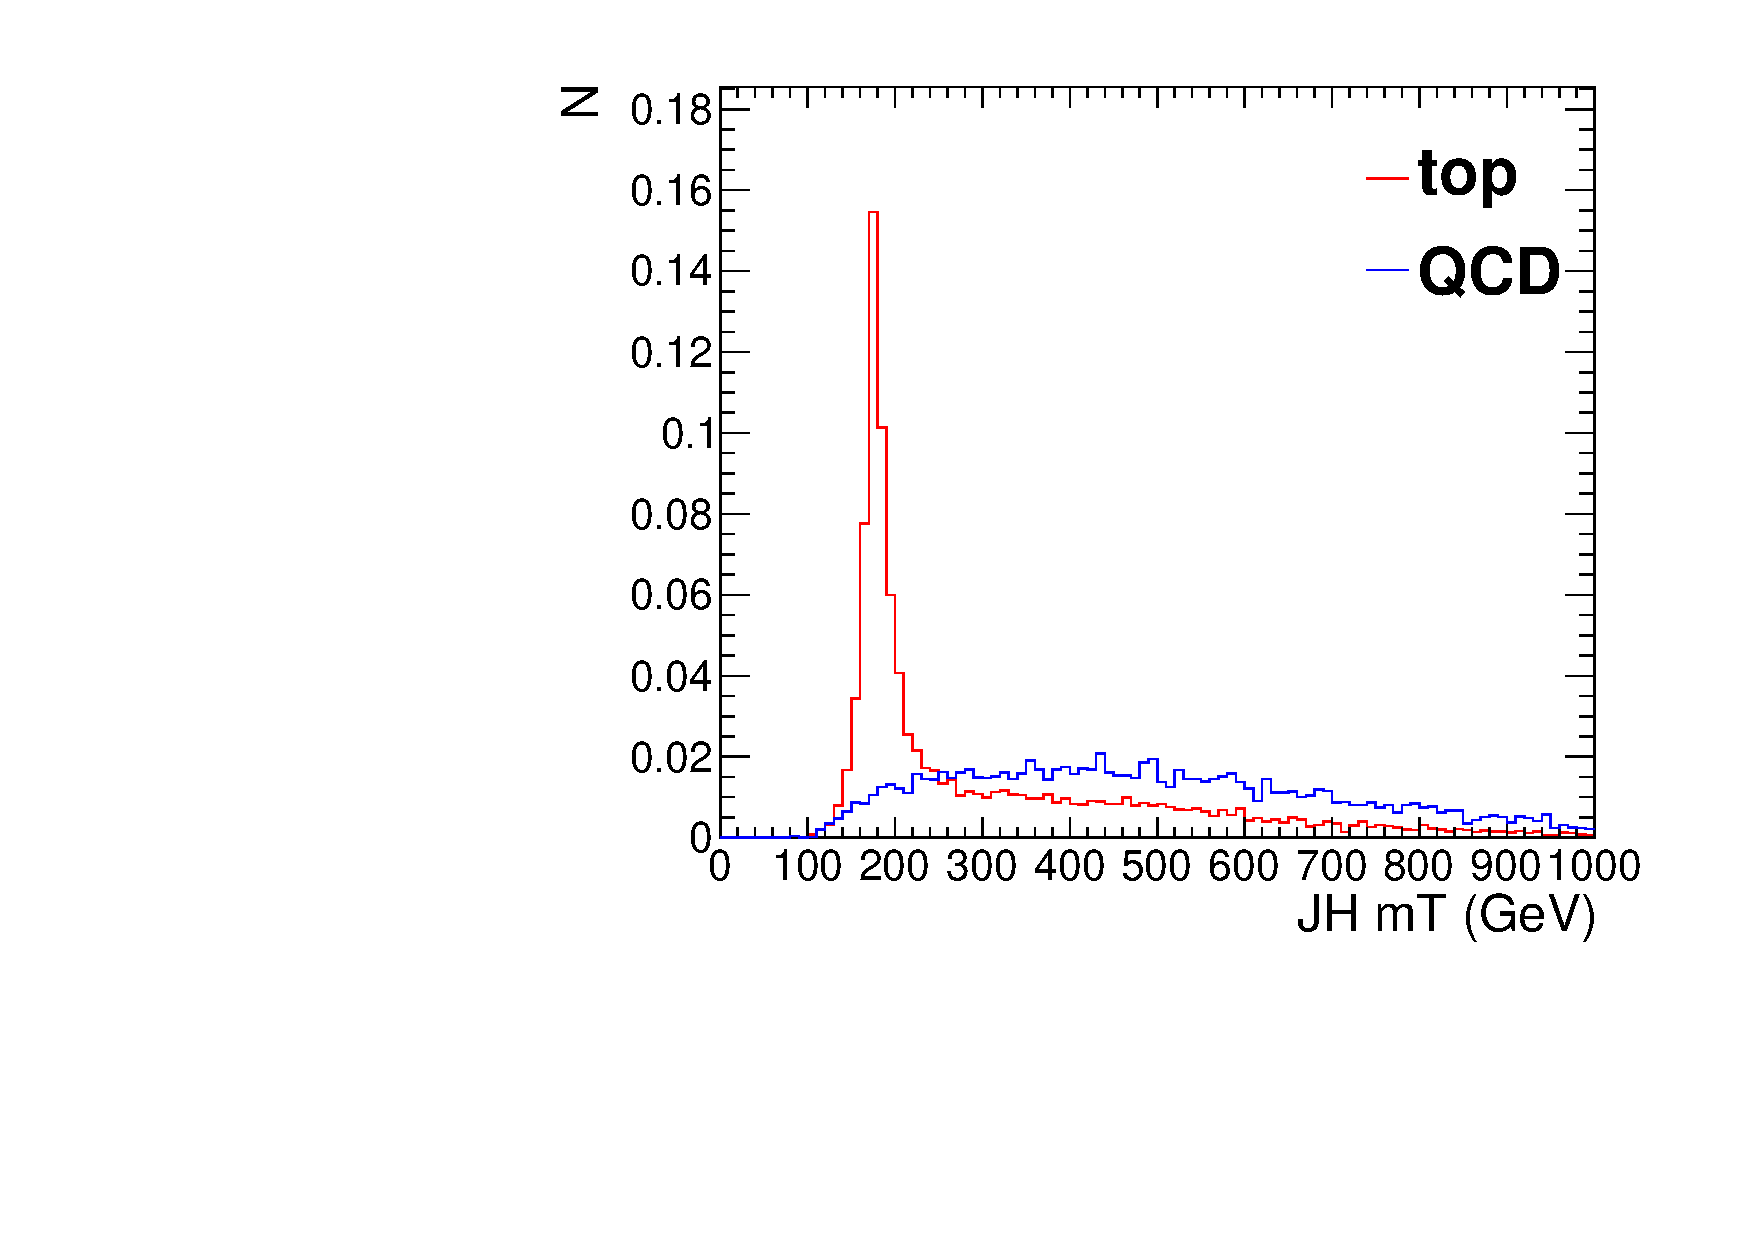
\includegraphics[width=0.48\textwidth]{./Figures/TTagging/single_variable/pT.1.5TeV.R.1.2/h_JH_mt_opt_all_once.pdf}}
\subfigure[HEPTopTagger, $R=1.2$]{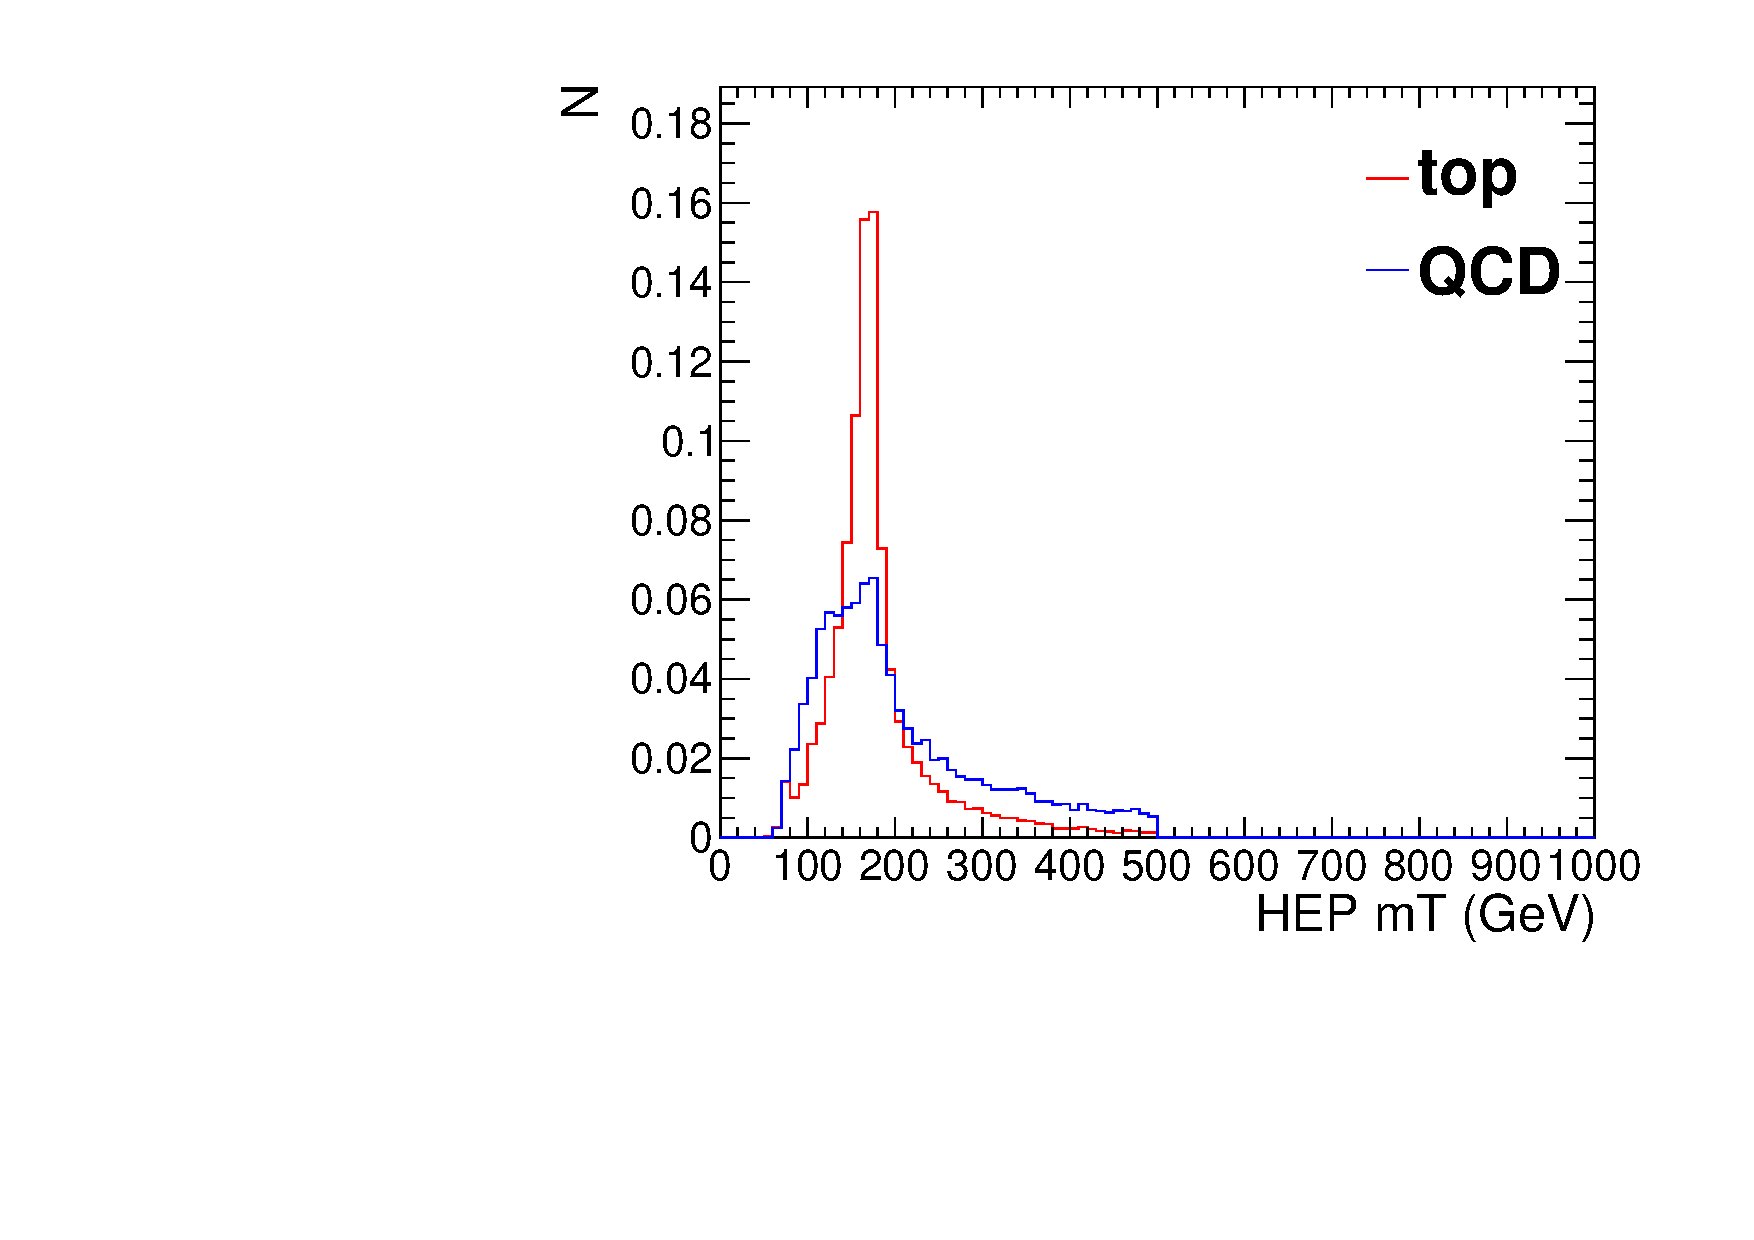
\includegraphics[width=0.48\textwidth]{./Figures/TTagging/single_variable/pT.1.5TeV.R.1.2/h_HEP_mt_opt_all_once.pdf}}
\caption{Comparison of individual jet shape performance at different \pt using the anti-\kT R=0.8 algorithm, $p_{\rm T}=1.5-1.6$ TeV. Each histogram is shown for the working point, optimized for best performance of the tagger for $p_{\rm T}=1-1.1$ GeV, at signal efficiency 0.3.}
\label{fig:topmass_histogram_optallonce_HEP_JH}
\end{center}
\end{figure*}



We also directly compare each variable's performance for different jet $\pt$ and radius. The results are shown in Figs.~\ref{fig:ptcomparison_singleshape_top}-\ref{fig:ptcomparison_singlewmass_top} for different $\pt$ bins and Figs.~\ref{fig:Rcomparison_singleshape_top}-\ref{fig:Rcomparison_singlewmass_top} for different $R$ values. The input parameters of the taggers, groomers, and shape variables are separately optimized for each $\pt$ and radius. If we only optimize the tagger inputs for one value of $\pt$ and $R$, the ROC curve behavior does not change substantially from one where the inputs are optimized at each $\pt$ and $R$ value; however, not all signal efficiencies are possible for every choice of tagger input, since the baseline selection efficiency might be too low. 


\begin{figure*}
\begin{center}
\subfigure[$C_2^{(\beta=1)}$]{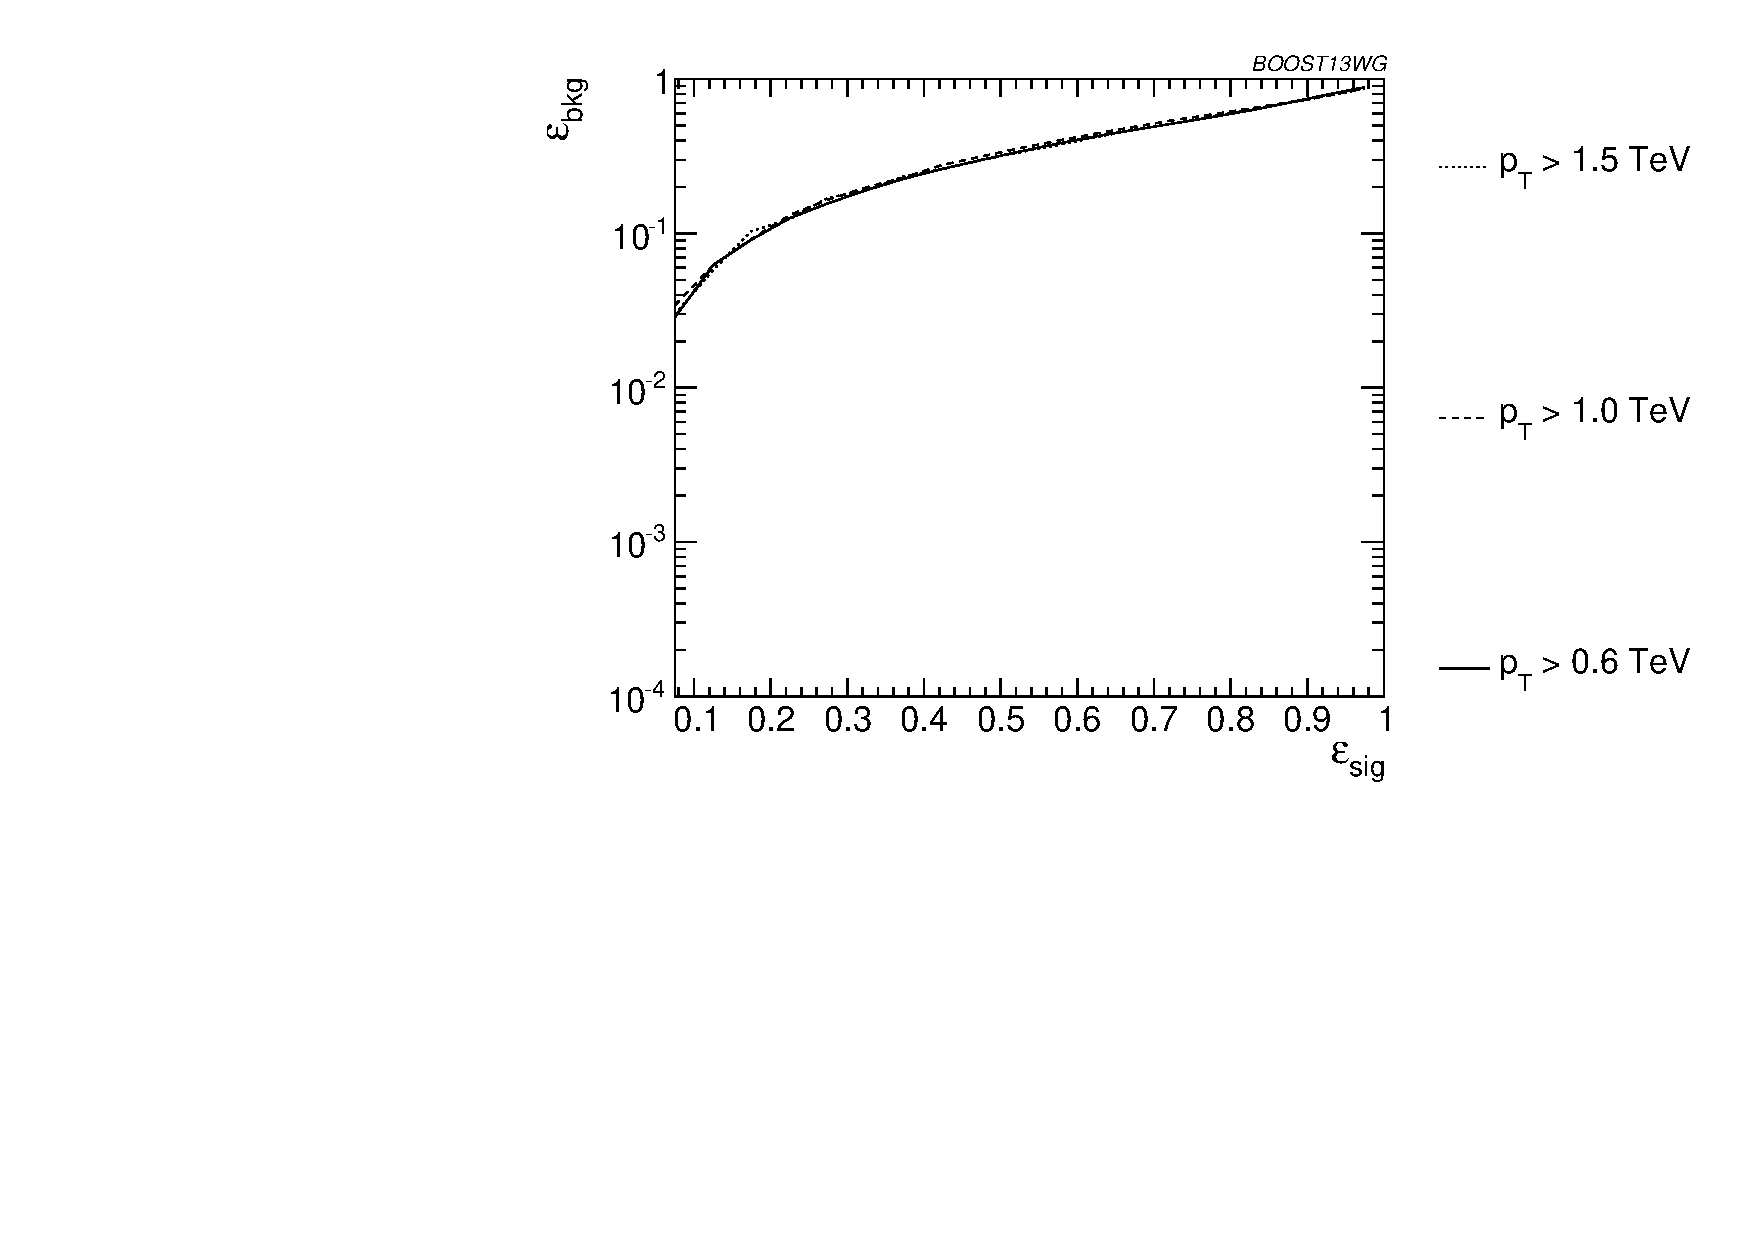
\includegraphics[width=0.48\textwidth]{./Figures/TTagging/single_variable/pT_compare/Rocs_C2b1_pTcompare.pdf}}
\subfigure[$C_3^{(\beta=1)}$]{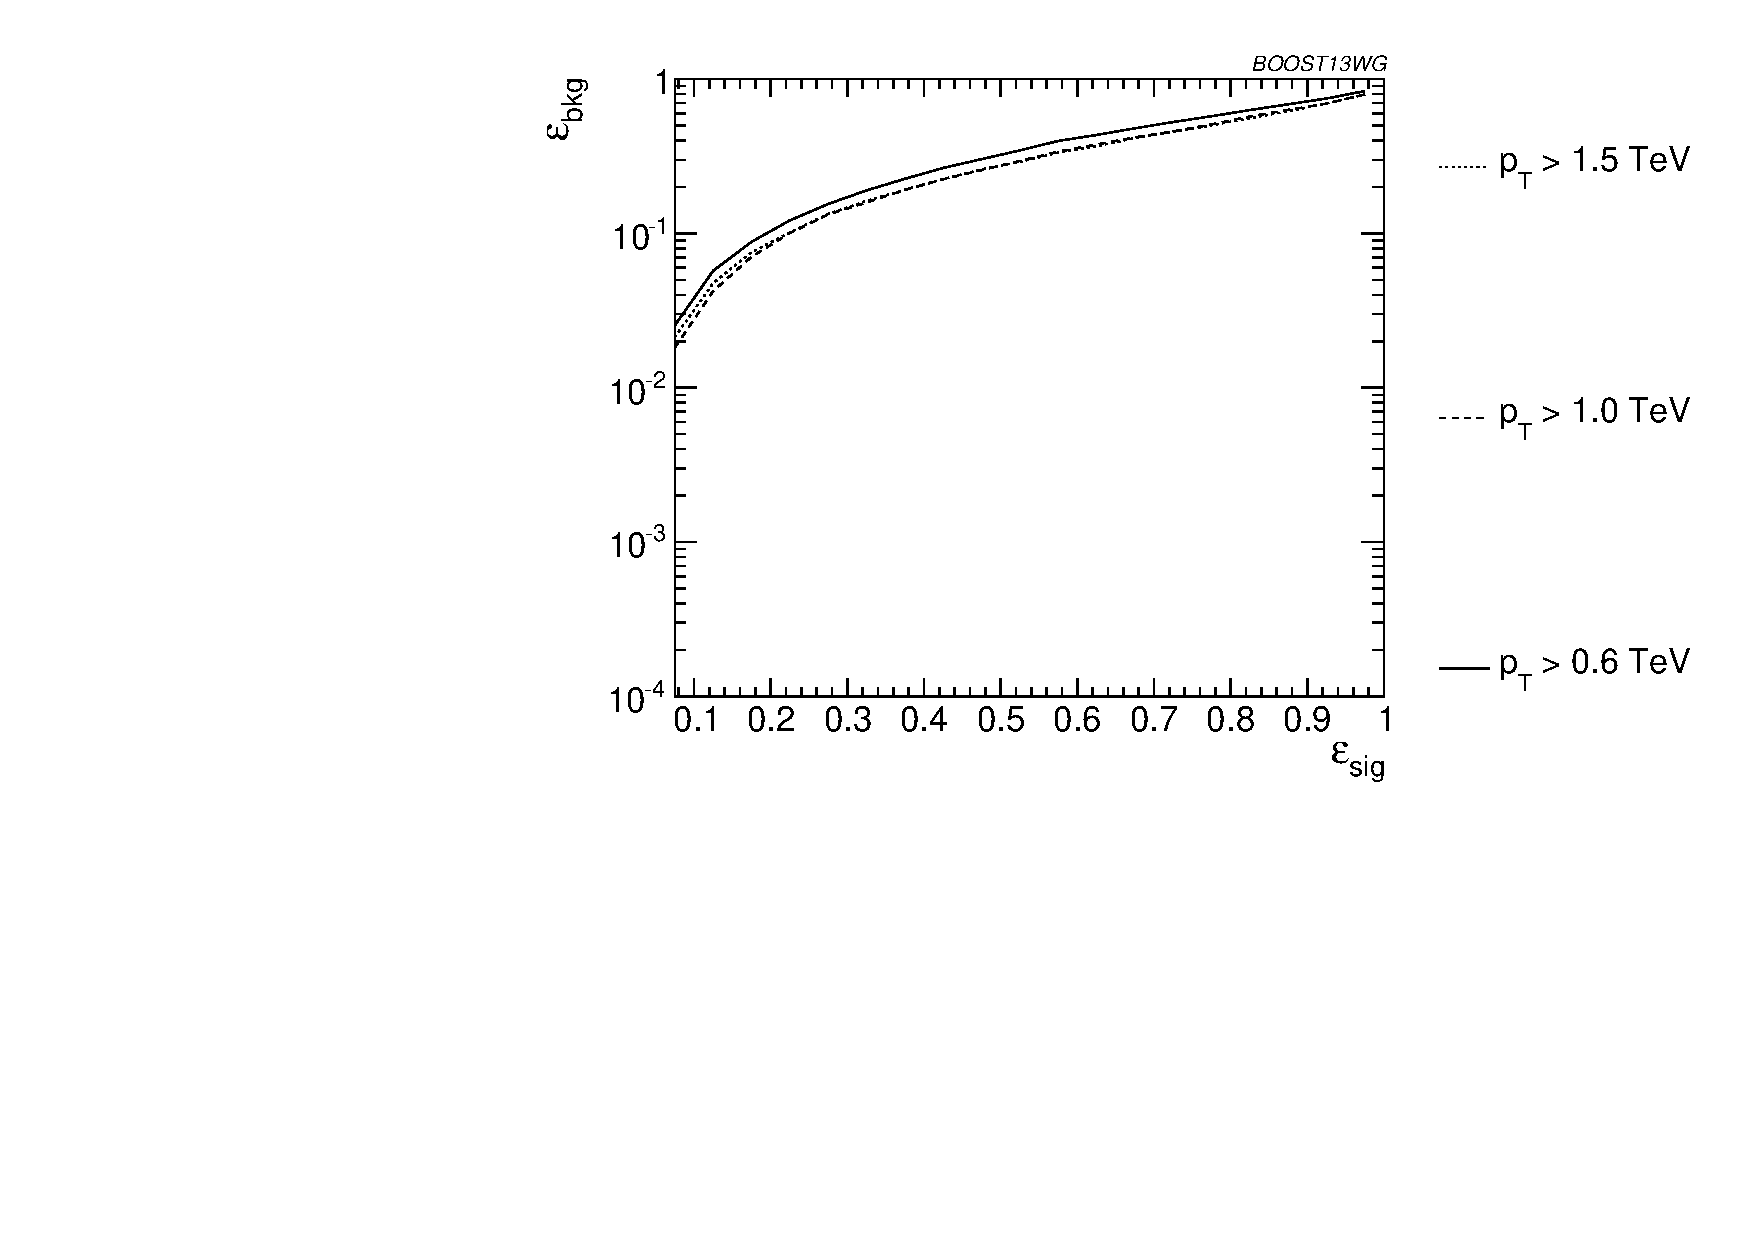
\includegraphics[width=0.48\textwidth]{./Figures/TTagging/single_variable/pT_compare/Rocs_C3b1_pTcompare.pdf}}
\subfigure[$\tau_{21}^{(\beta=1)}$]{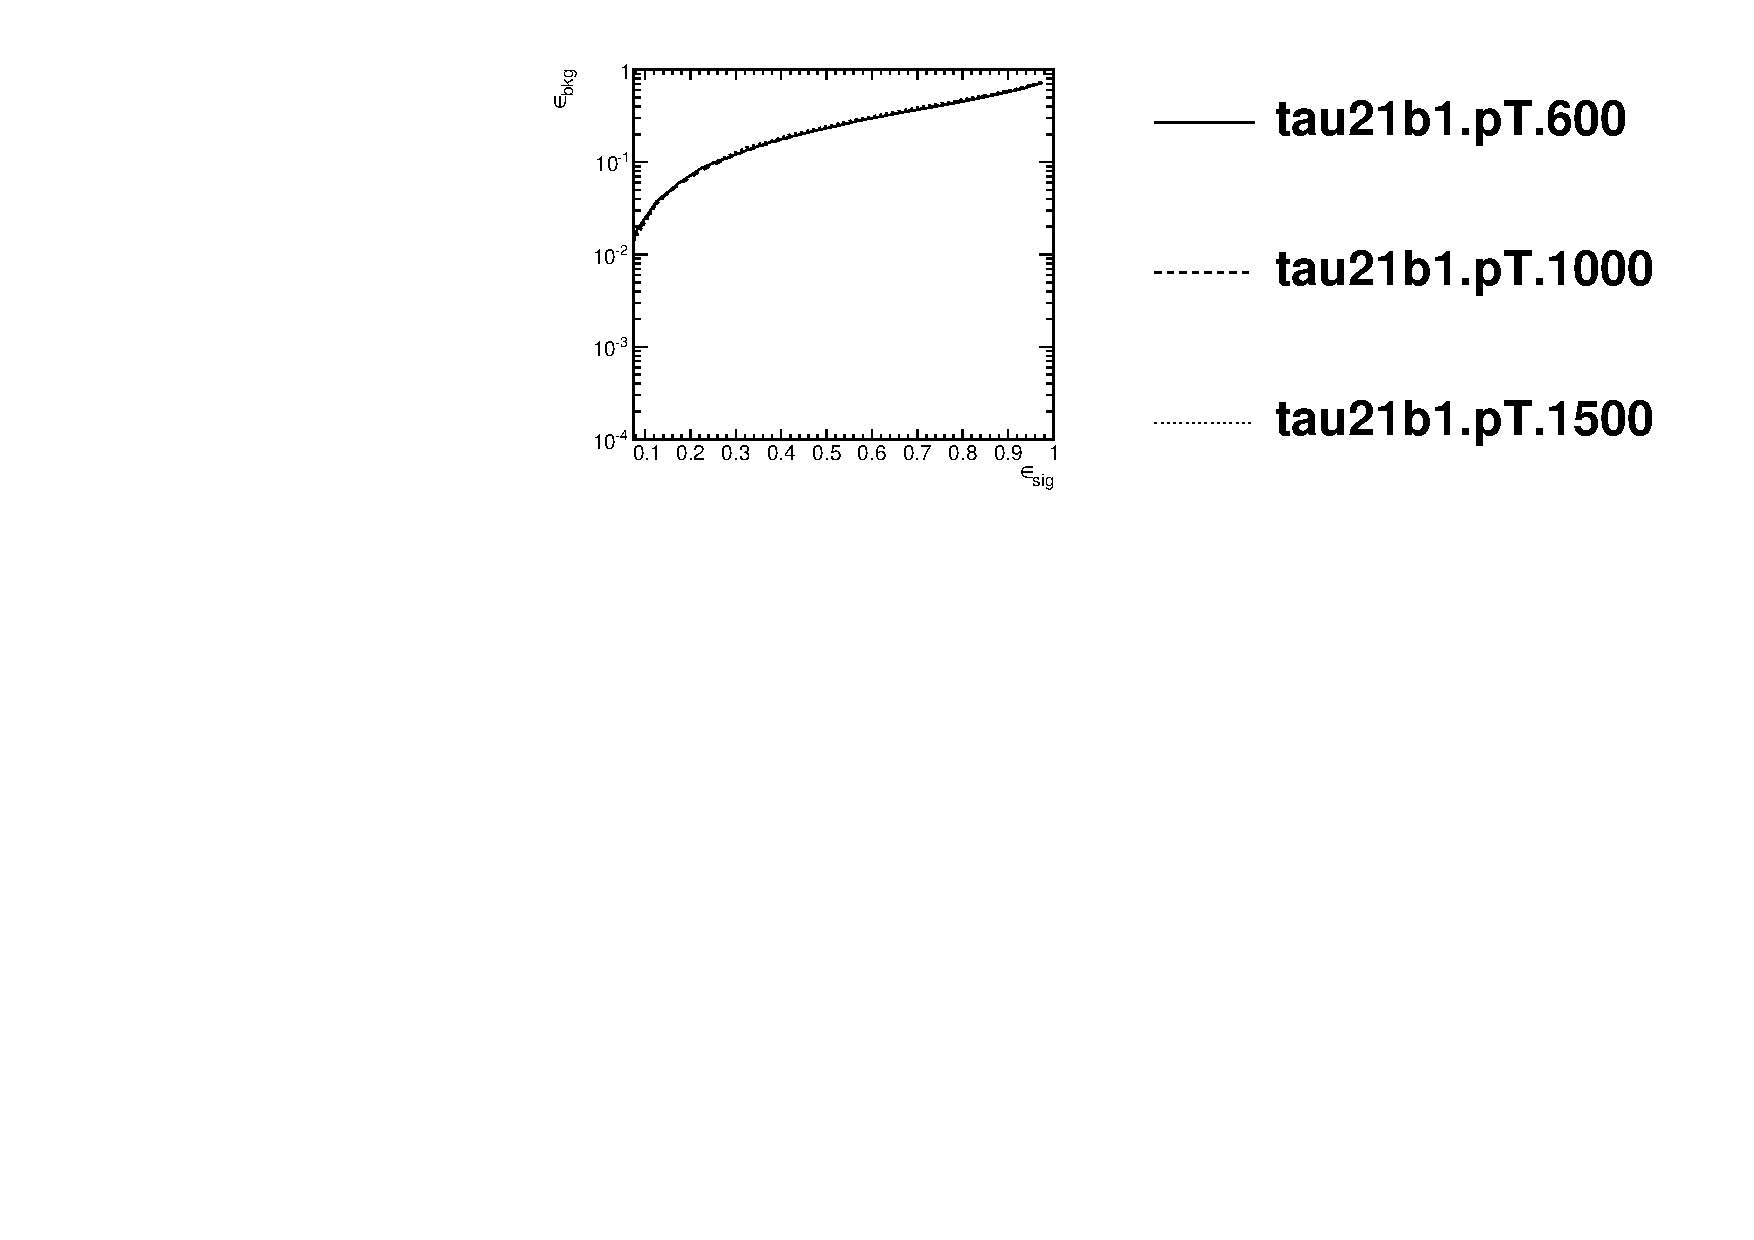
\includegraphics[width=0.48\textwidth]{./Figures/TTagging/single_variable/pT_compare/Rocs_tau21b1_pTcompare.pdf}}
\subfigure[$\tau_{32}^{(\beta=1)}$]{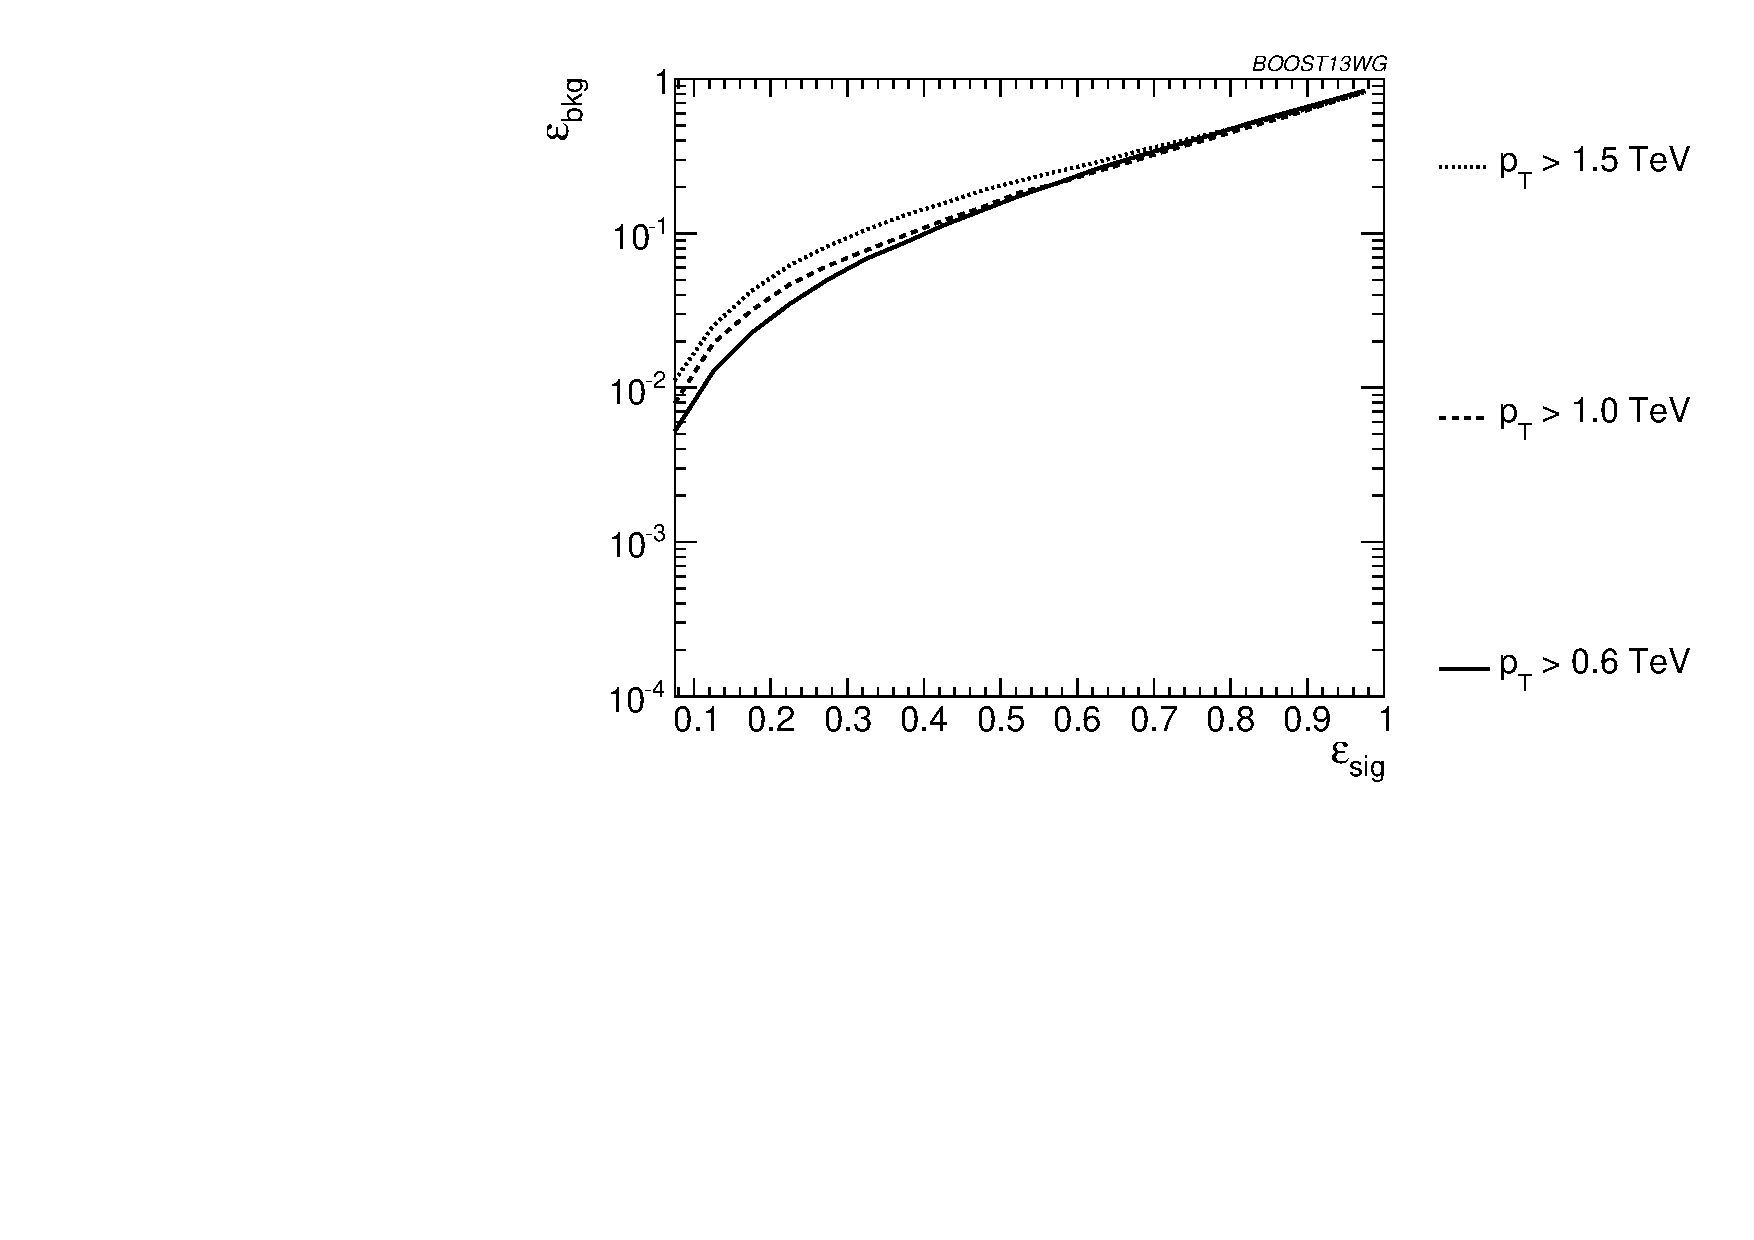
\includegraphics[width=0.48\textwidth]{./Figures/TTagging/single_variable/pT_compare/Rocs_tau32b1_pTcompare.pdf}}
\subfigure[Qjet mass volatility]{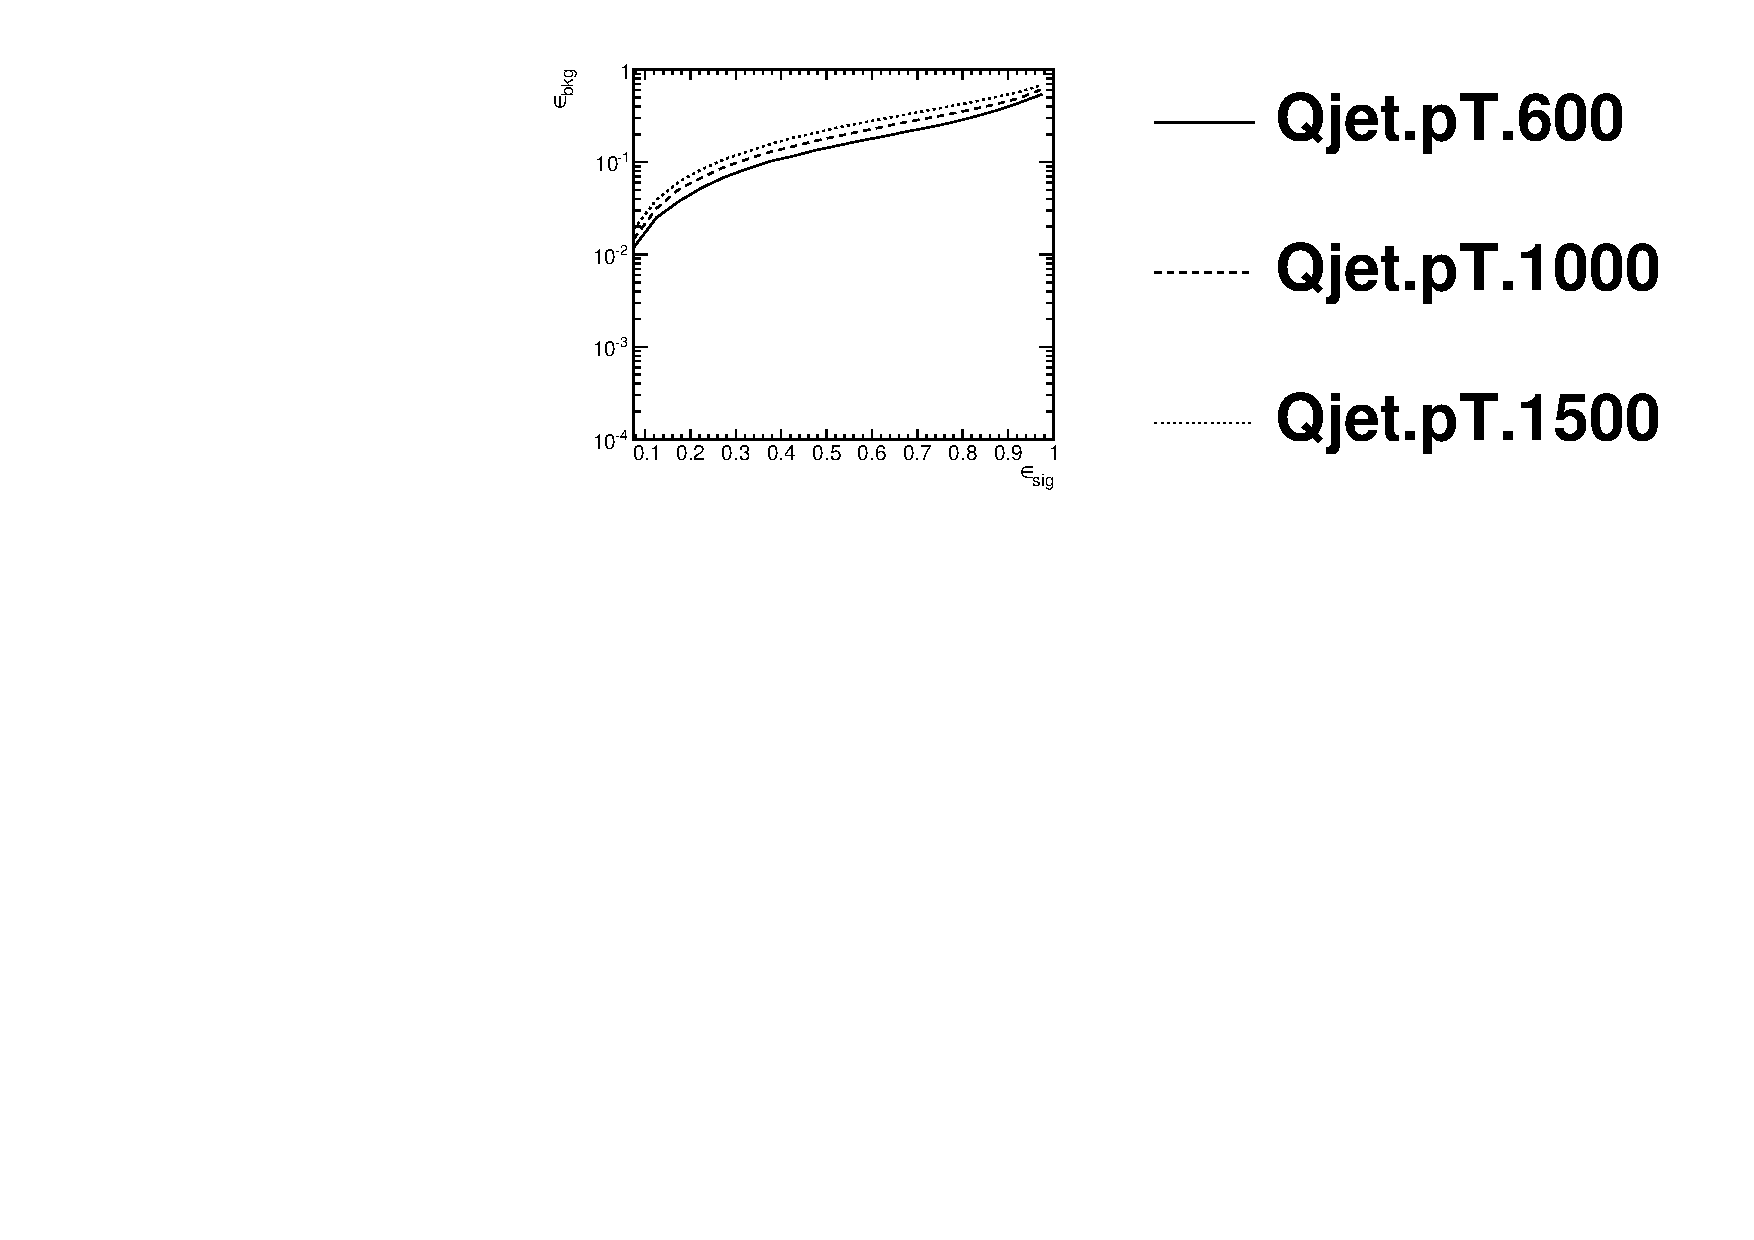
\includegraphics[width=0.48\textwidth]{./Figures/TTagging/single_variable/pT_compare/Rocs_Qjet_pTcompare.pdf}}
\caption{Comparison of individual jet shape performance at different \pt using the anti-\kT R=0.8 algorithm.}
\label{fig:ptcomparison_singleshape_top}
\end{center}
\end{figure*}

\begin{figure*}
\begin{center}
\subfigure[HEPTopTagger $m_t$]{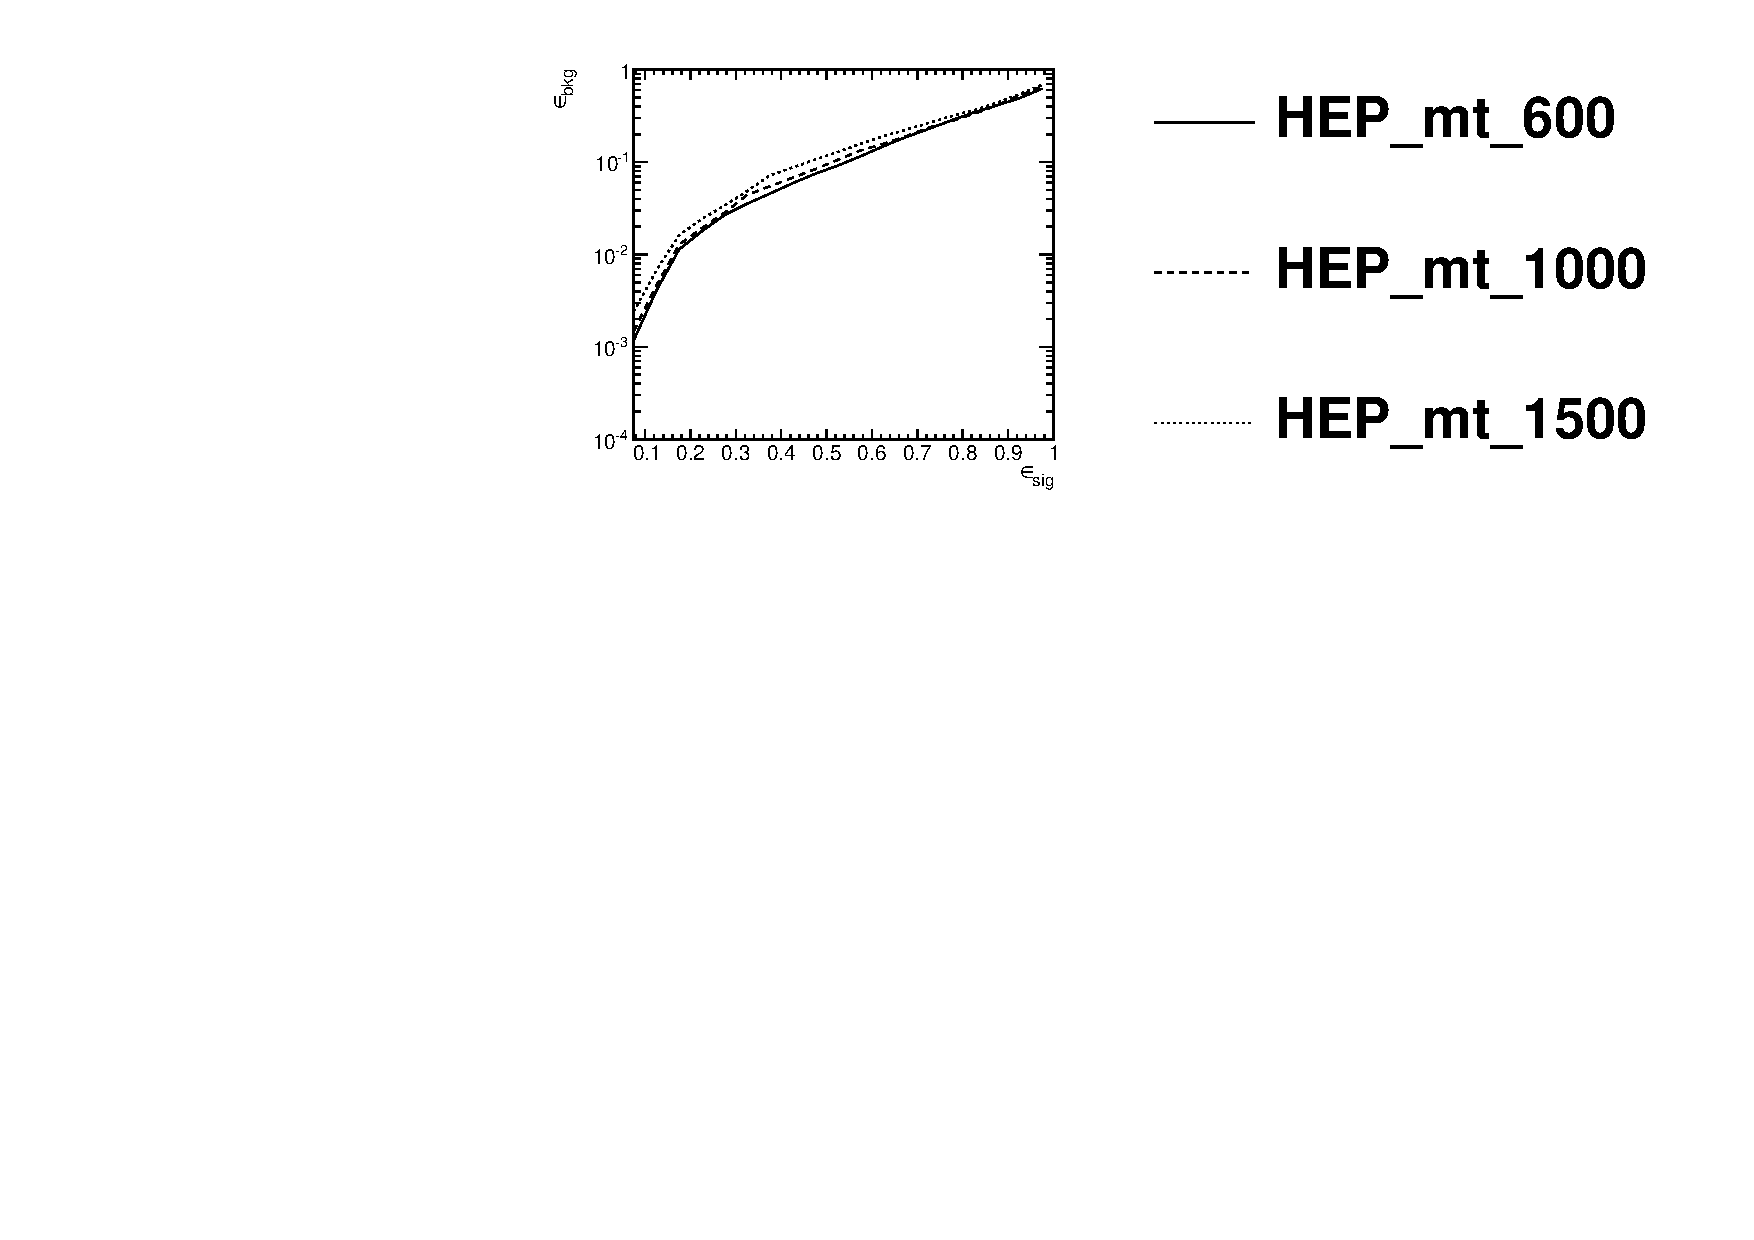
\includegraphics[width=0.48\textwidth]{./Figures/TTagging/single_variable/pT_compare/Rocs_HEP_mt_pTcompare.pdf}}
\subfigure[Johns Hopkins Tagger $m_t$]{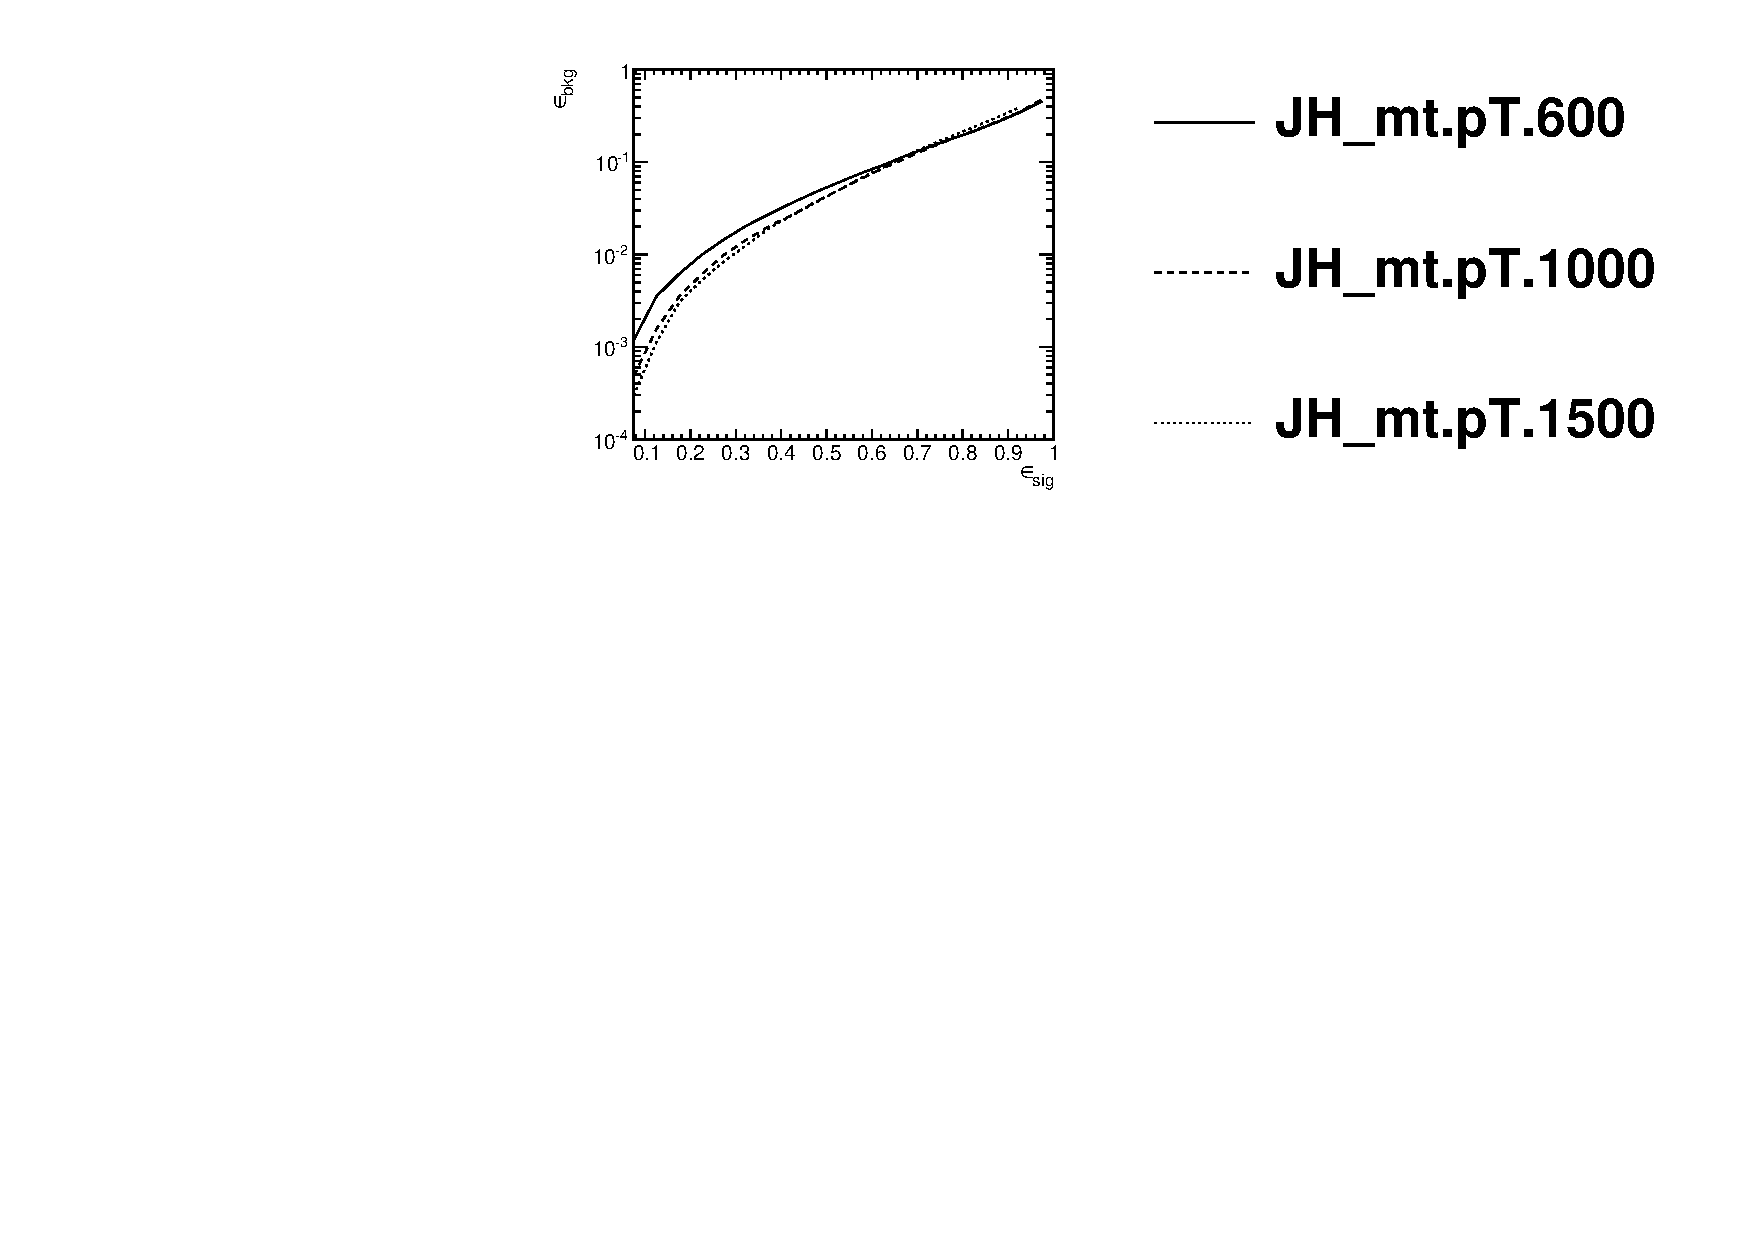
\includegraphics[width=0.48\textwidth]{./Figures/TTagging/single_variable/pT_compare/Rocs_JH_mt_pTcompare.pdf}}
\subfigure[Pruning $m_t$]{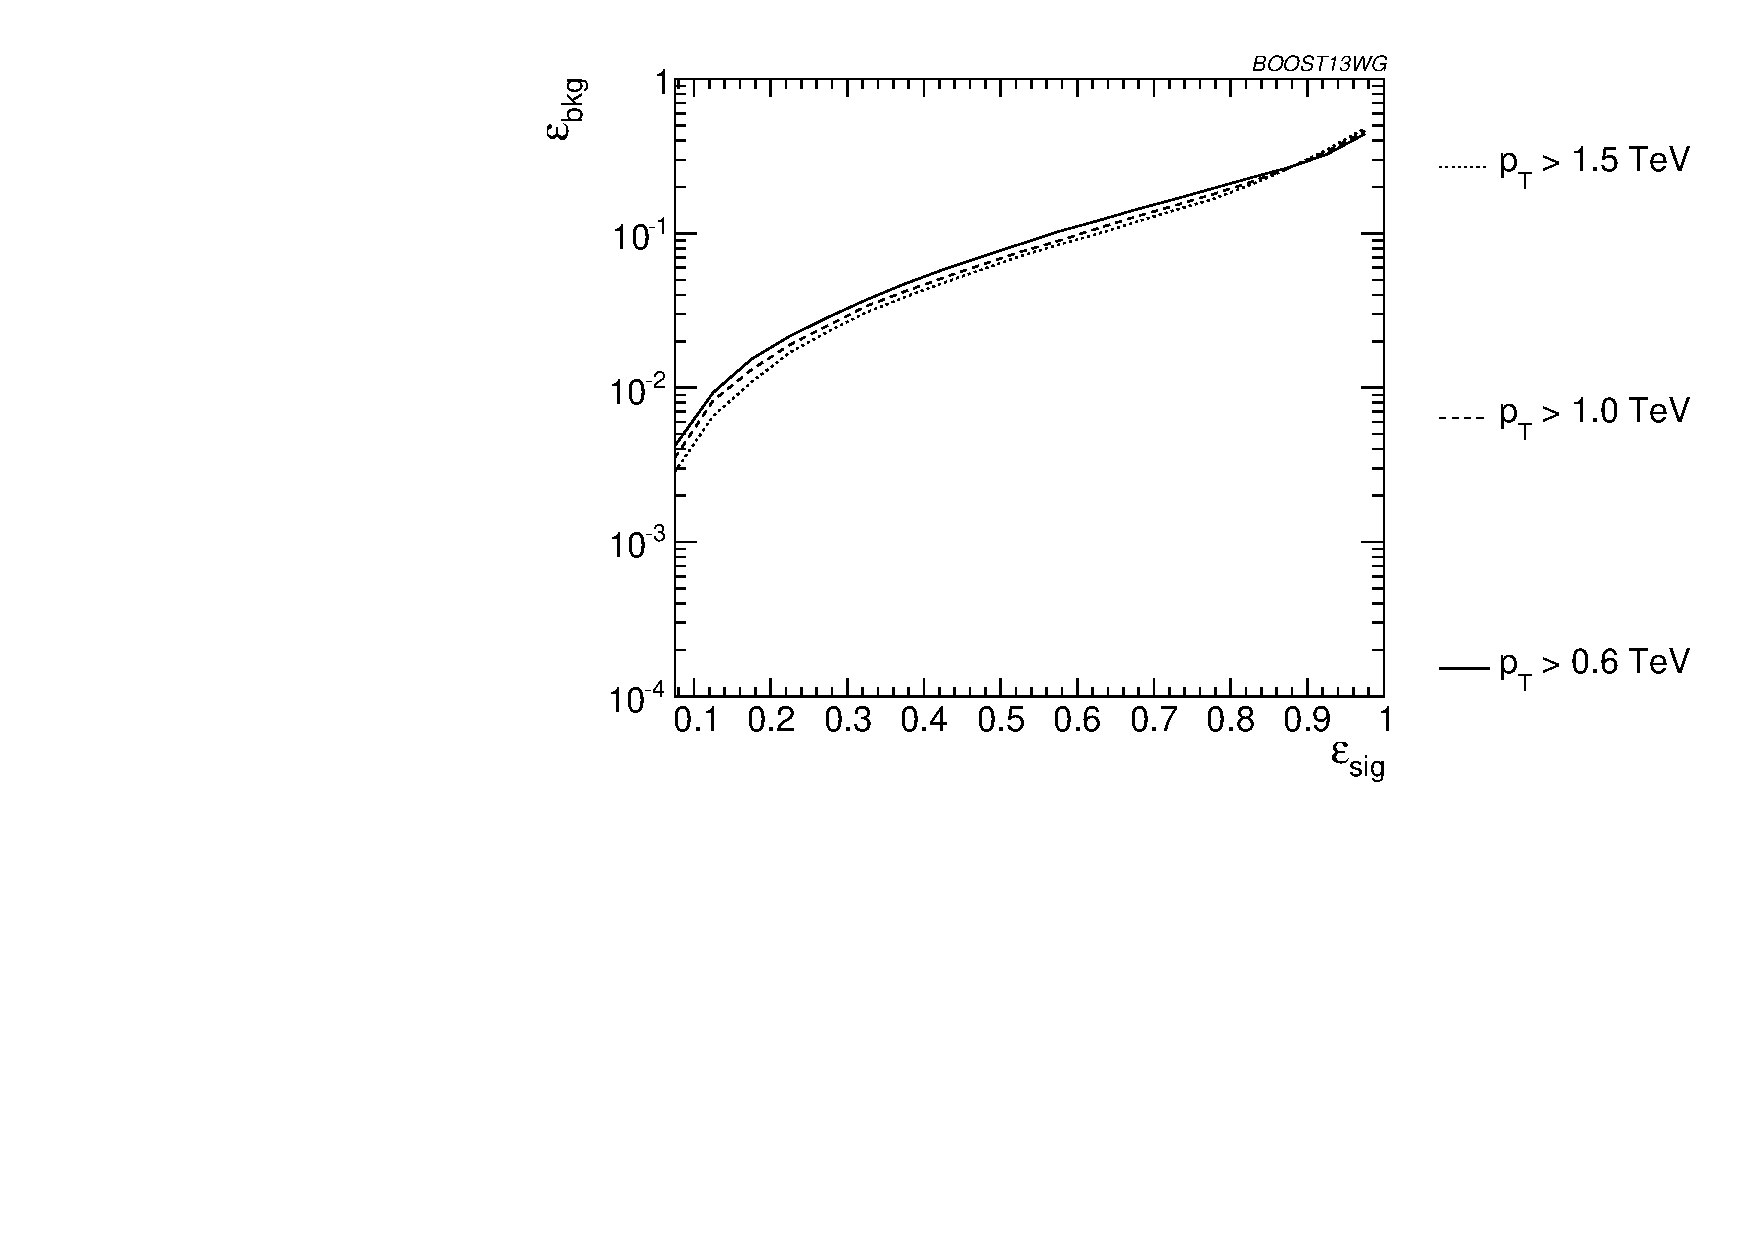
\includegraphics[width=0.48\textwidth]{./Figures/TTagging/single_variable/pT_compare/Rocs_prune_pTcompare.pdf}}
\subfigure[Trimming $m_t$]{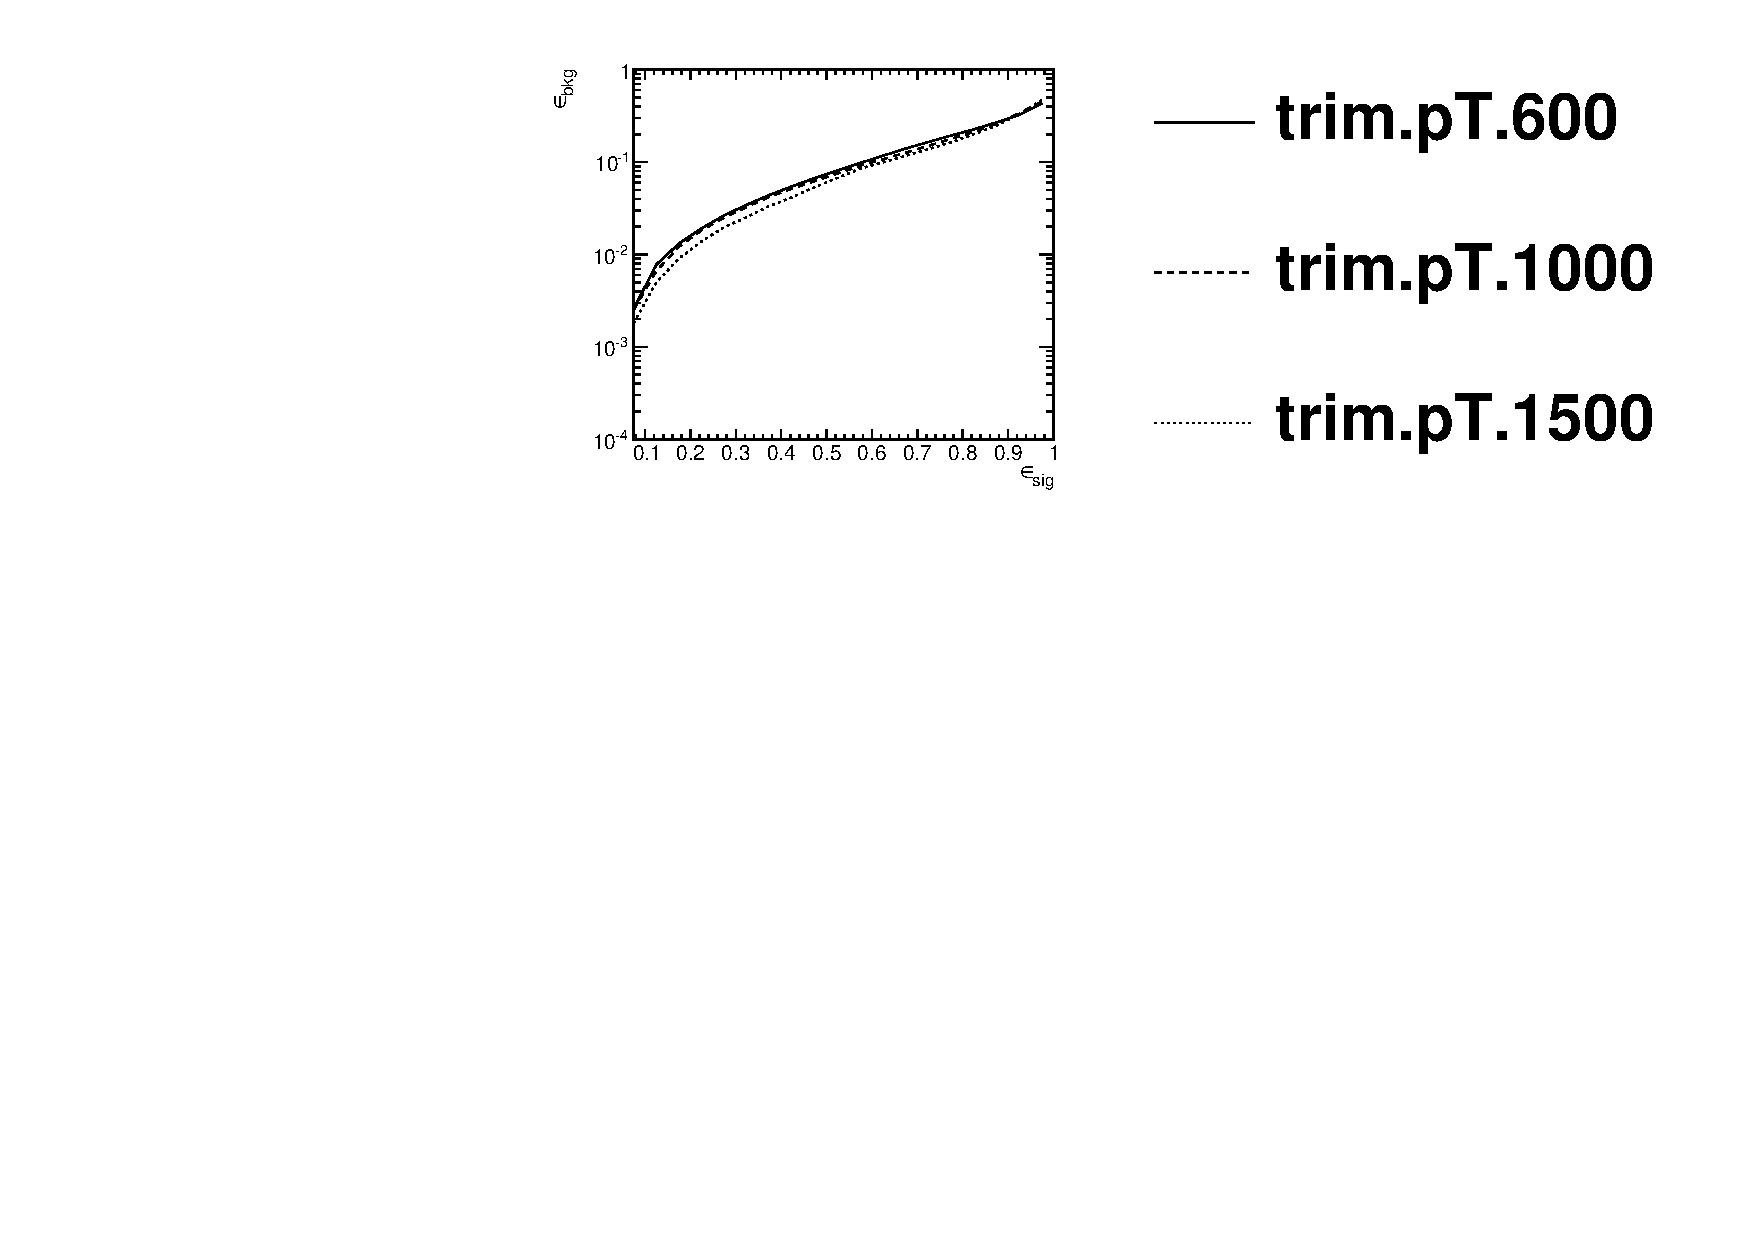
\includegraphics[width=0.48\textwidth]{./Figures/TTagging/single_variable/pT_compare/Rocs_trim_pTcompare.pdf}}
\caption{Comparison of top mass performance of different taggers at different \pt using the anti-\kT R=0.8 algorithm.}
\label{fig:ptcomparison_singletopmass_top}
\end{center}
\end{figure*}

\begin{figure*}
\begin{center}
\subfigure[HEPTopTagger $m_W$]{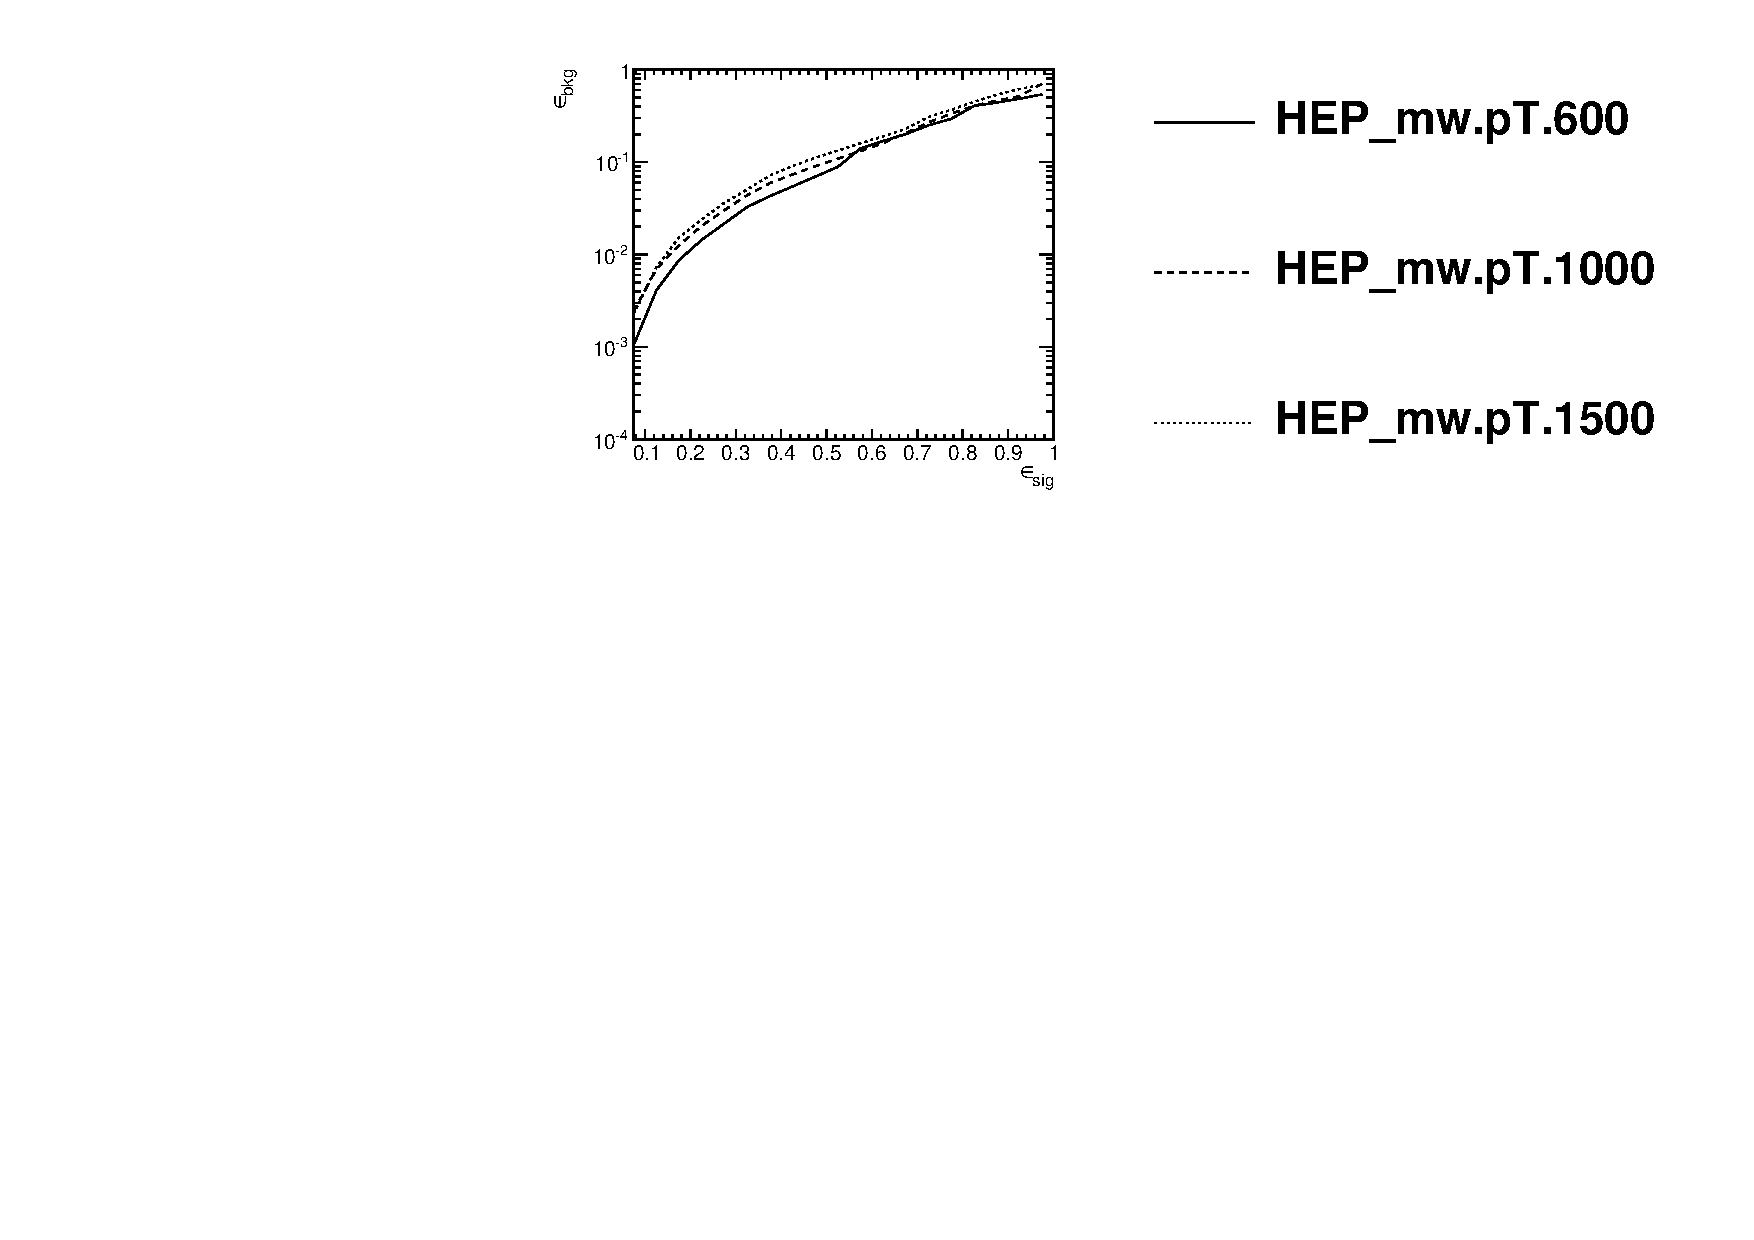
\includegraphics[width=0.48\textwidth]{./Figures/TTagging/single_variable/pT_compare/Rocs_HEP_mw_pTcompare.pdf}}
\subfigure[Johns Hopkins Tagger $m_W$]{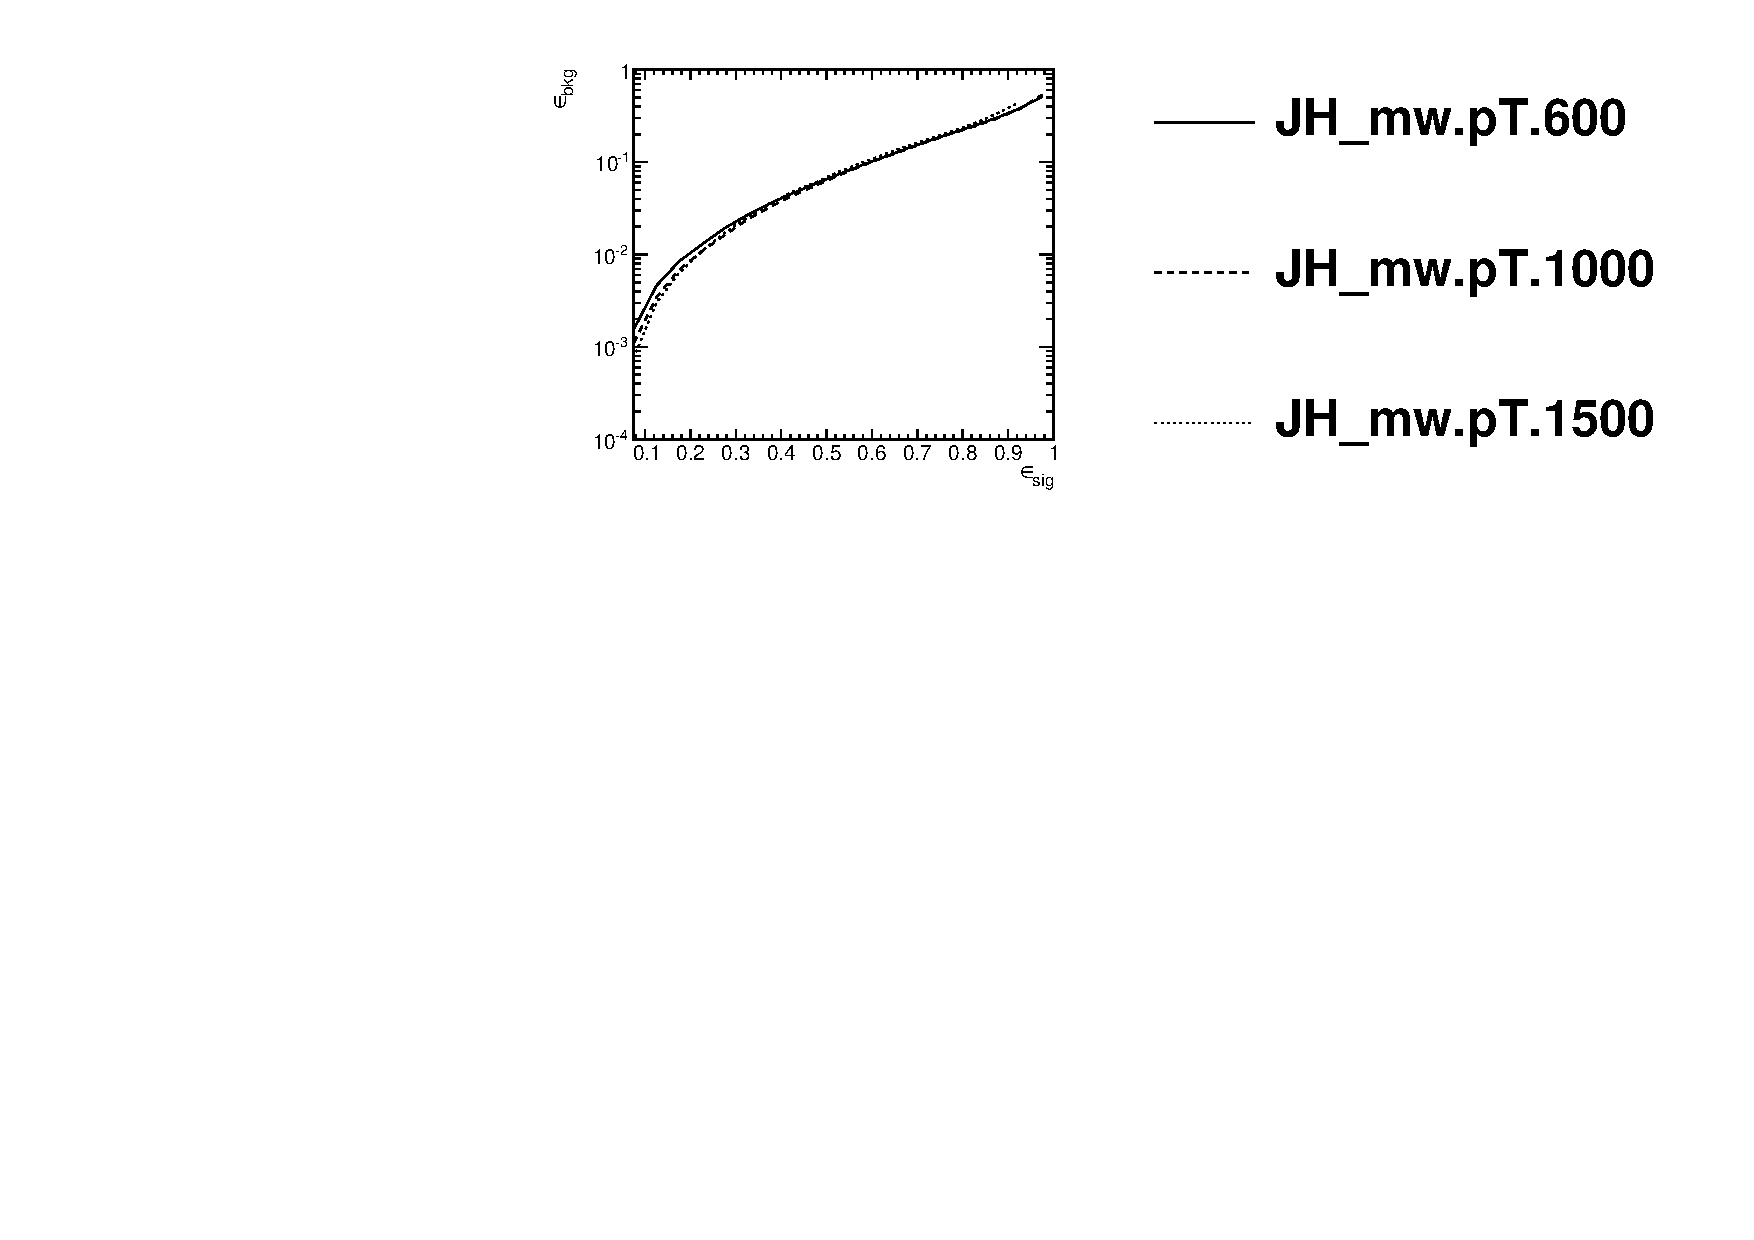
\includegraphics[width=0.48\textwidth]{./Figures/TTagging/single_variable/pT_compare/Rocs_JH_mw_pTcompare.pdf}}
\subfigure[Pruning $m_W$]{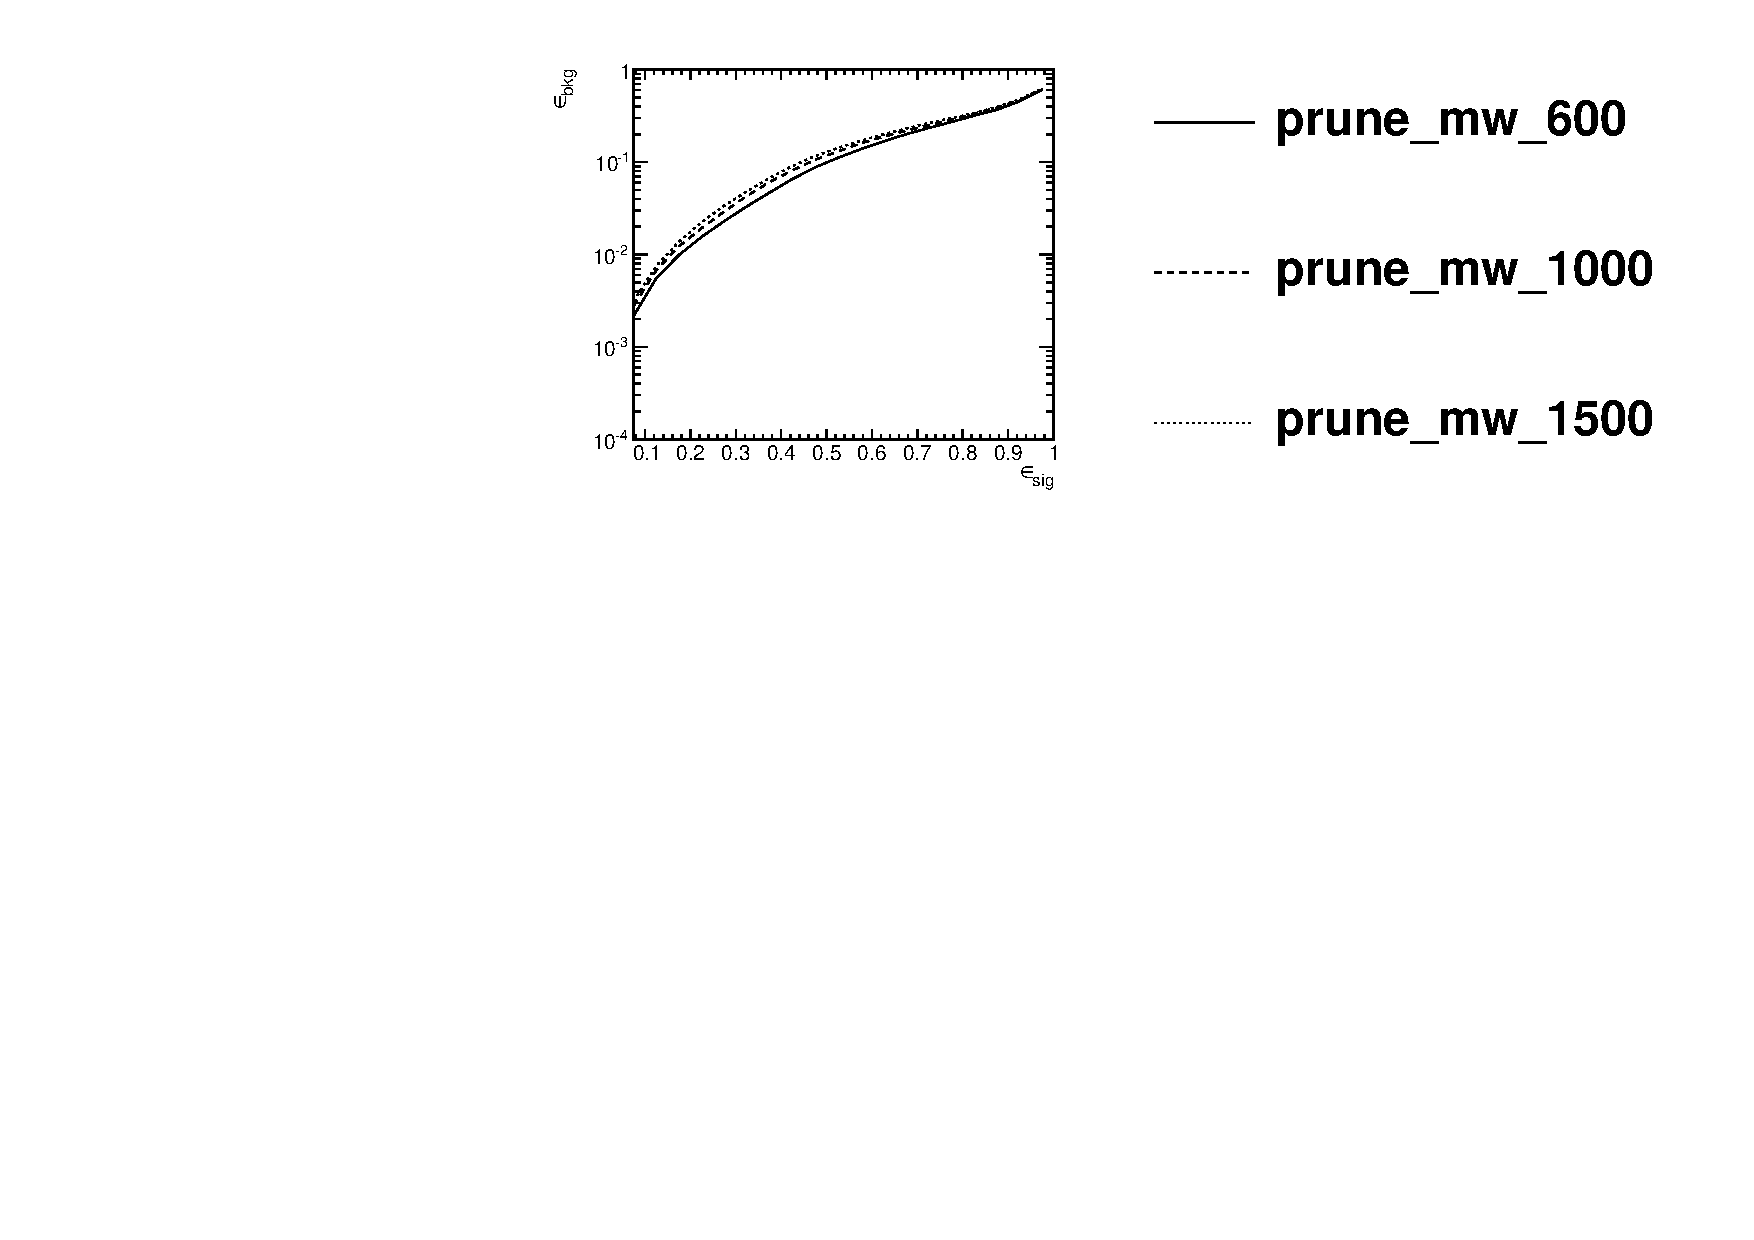
\includegraphics[width=0.48\textwidth]{./Figures/TTagging/single_variable/pT_compare/Rocs_prune_mw_pTcompare.pdf}}
\subfigure[Trimming $m_W$]{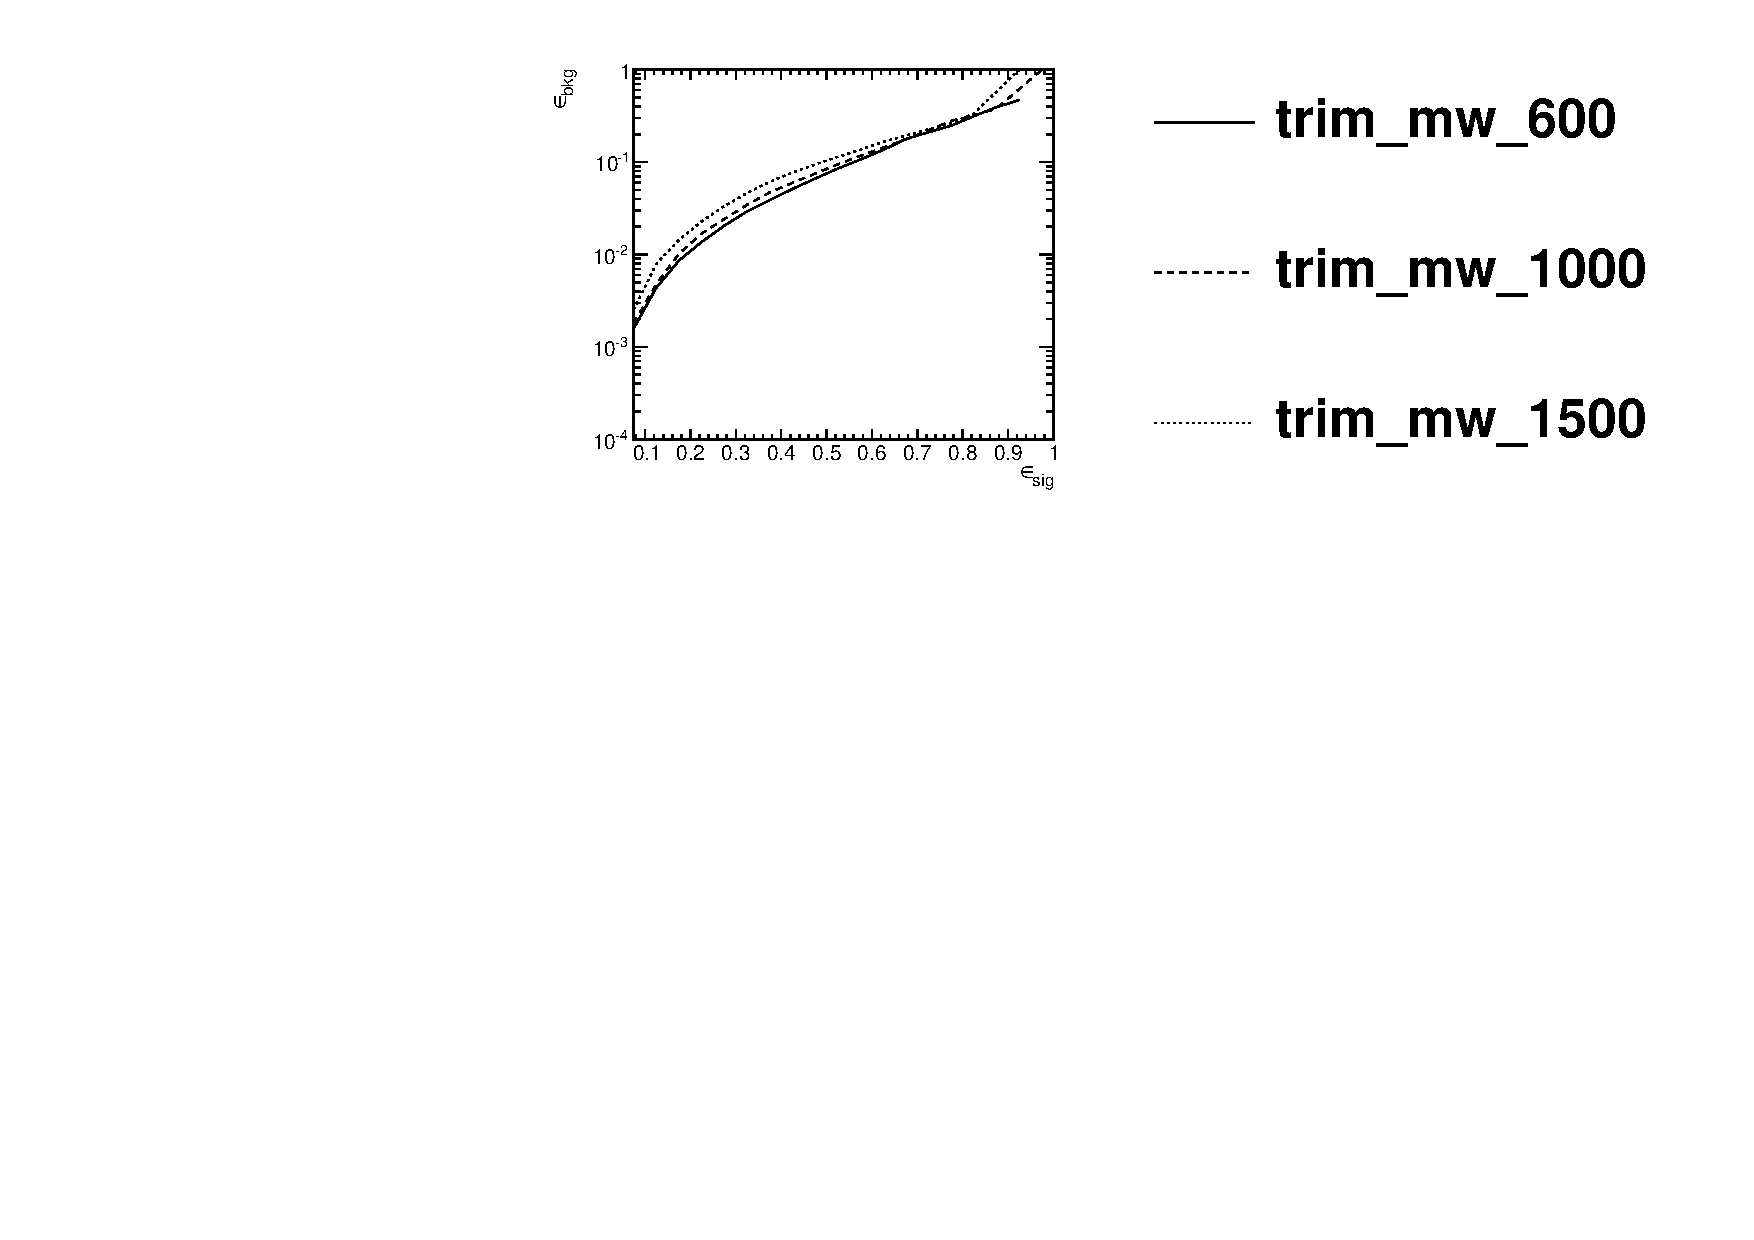
\includegraphics[width=0.48\textwidth]{./Figures/TTagging/single_variable/pT_compare/Rocs_trim_mw_pTcompare.pdf}}
\caption{Comparison of $W$ mass performance of different taggers at different \pt using the anti-\kT R=0.8 algorithm.}
\label{fig:ptcomparison_singlewmass_top}
\end{center}
\end{figure*}

\begin{figure*}
\begin{center}
\subfigure[$C_2^{(\beta=1)}$]{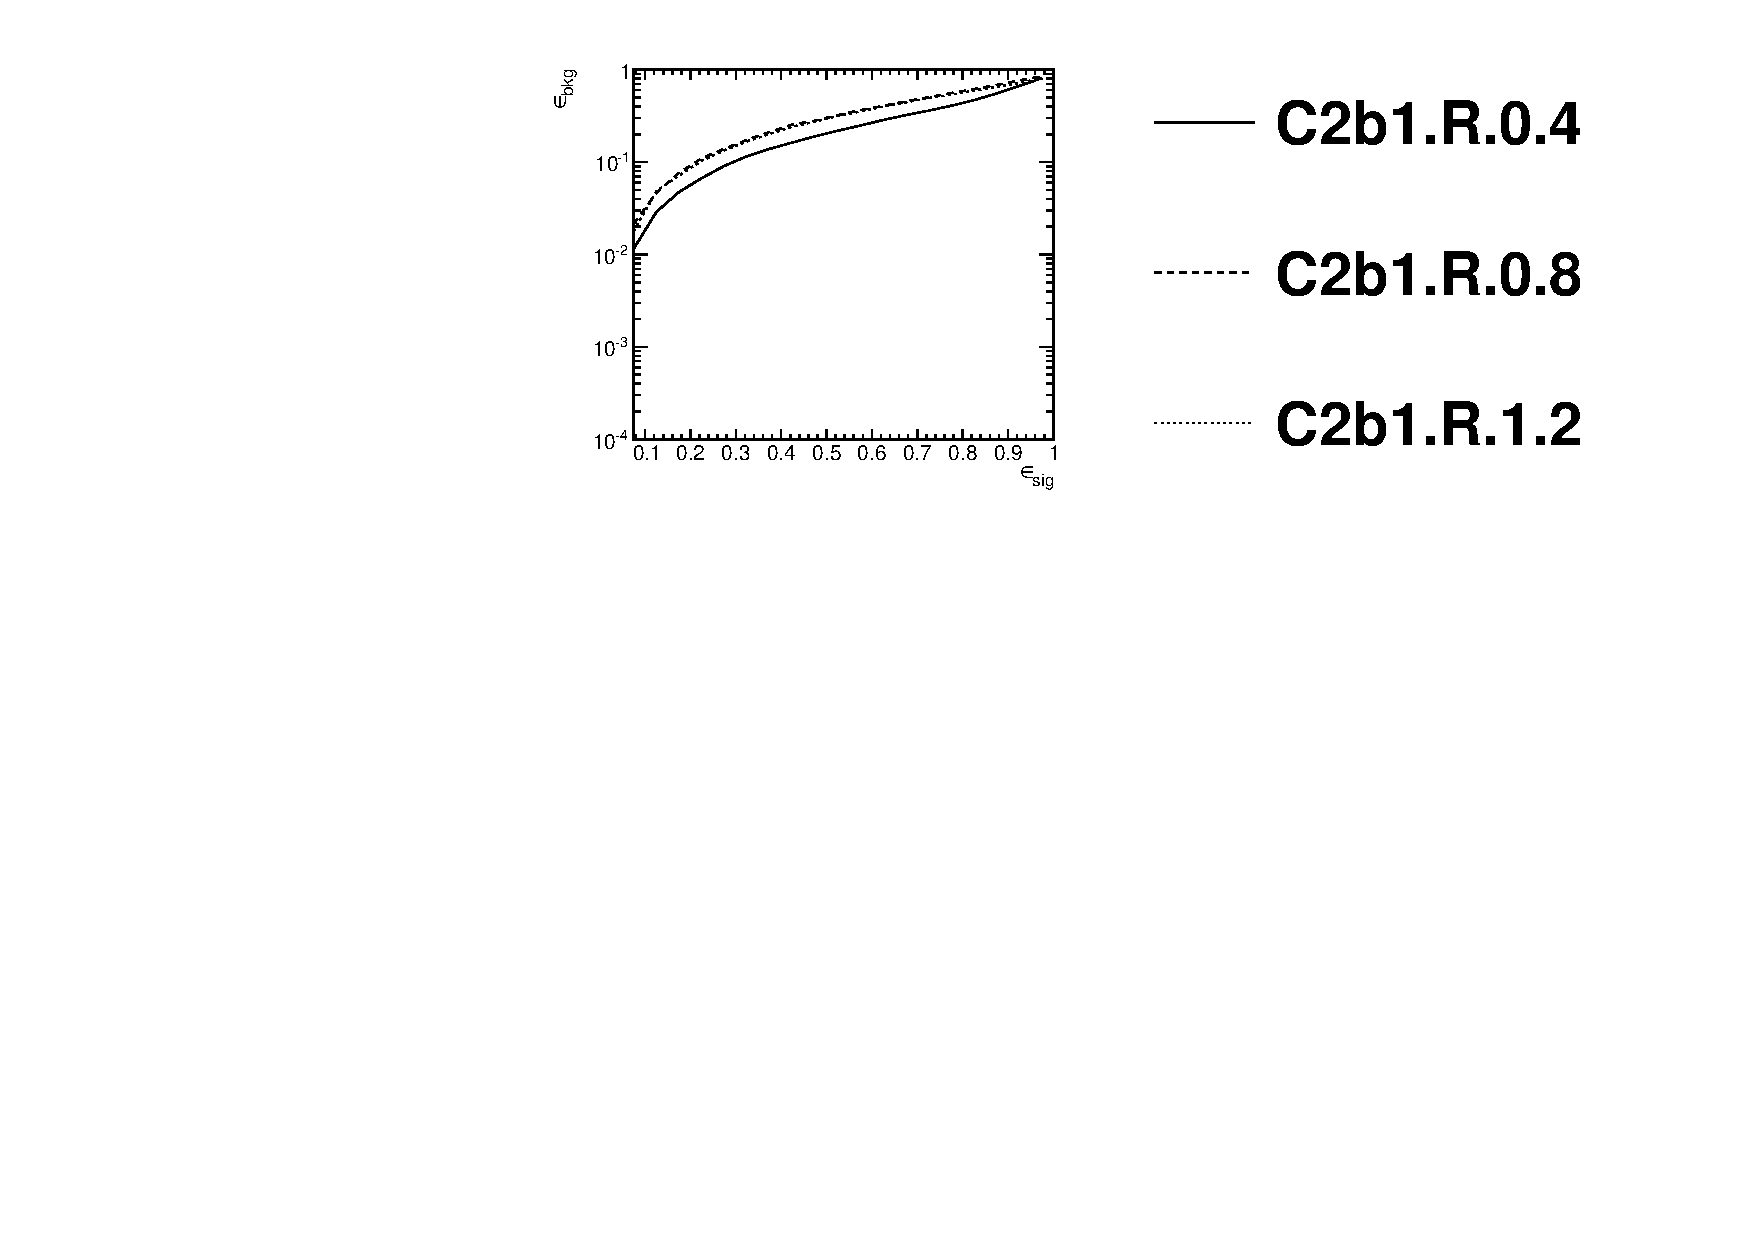
\includegraphics[width=0.48\textwidth]{./Figures/TTagging/single_variable/R_compare/Rocs_C2b1_Rcompare.pdf}}
\subfigure[$C_3^{(\beta=1)}$]{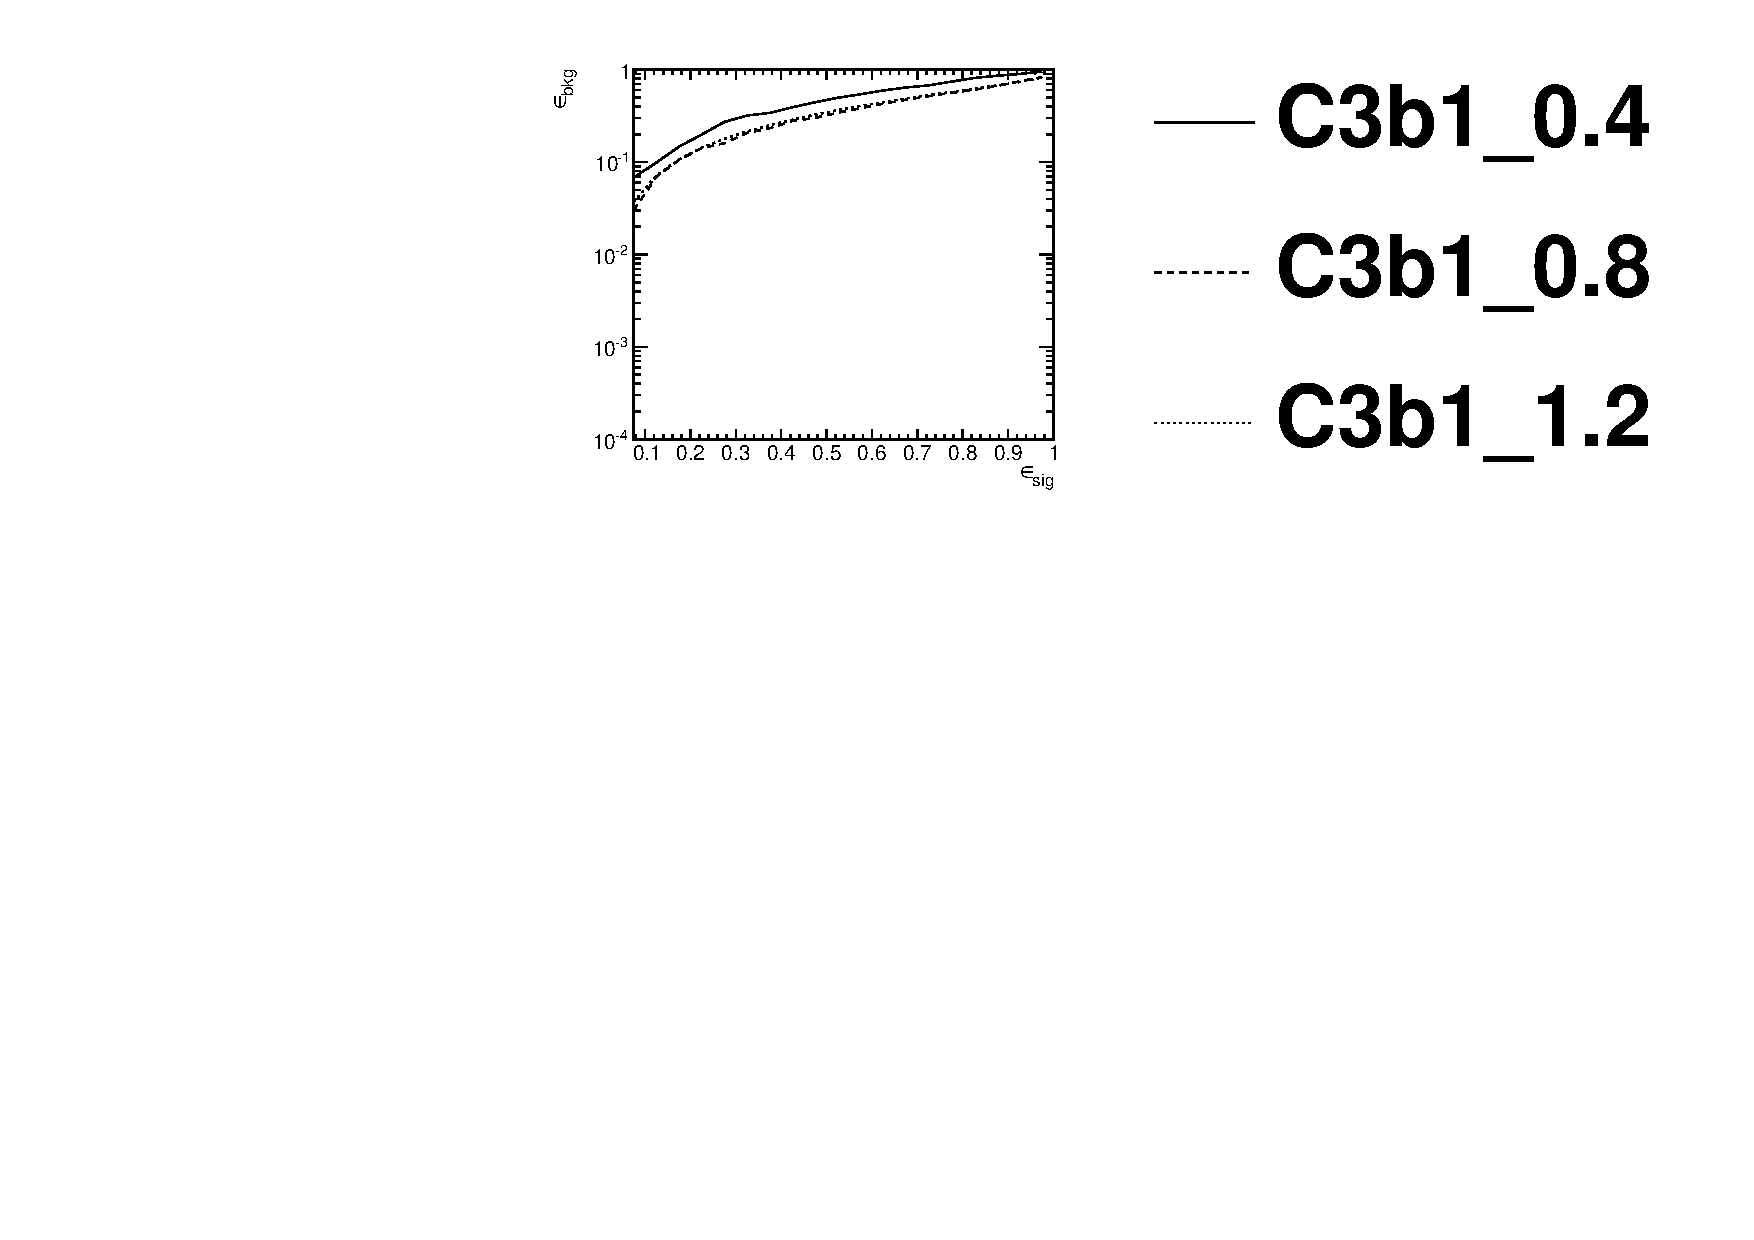
\includegraphics[width=0.48\textwidth]{./Figures/TTagging/single_variable/R_compare/Rocs_C3b1_Rcompare.pdf}}
\subfigure[$\tau_{21}^{(\beta=1)}$]{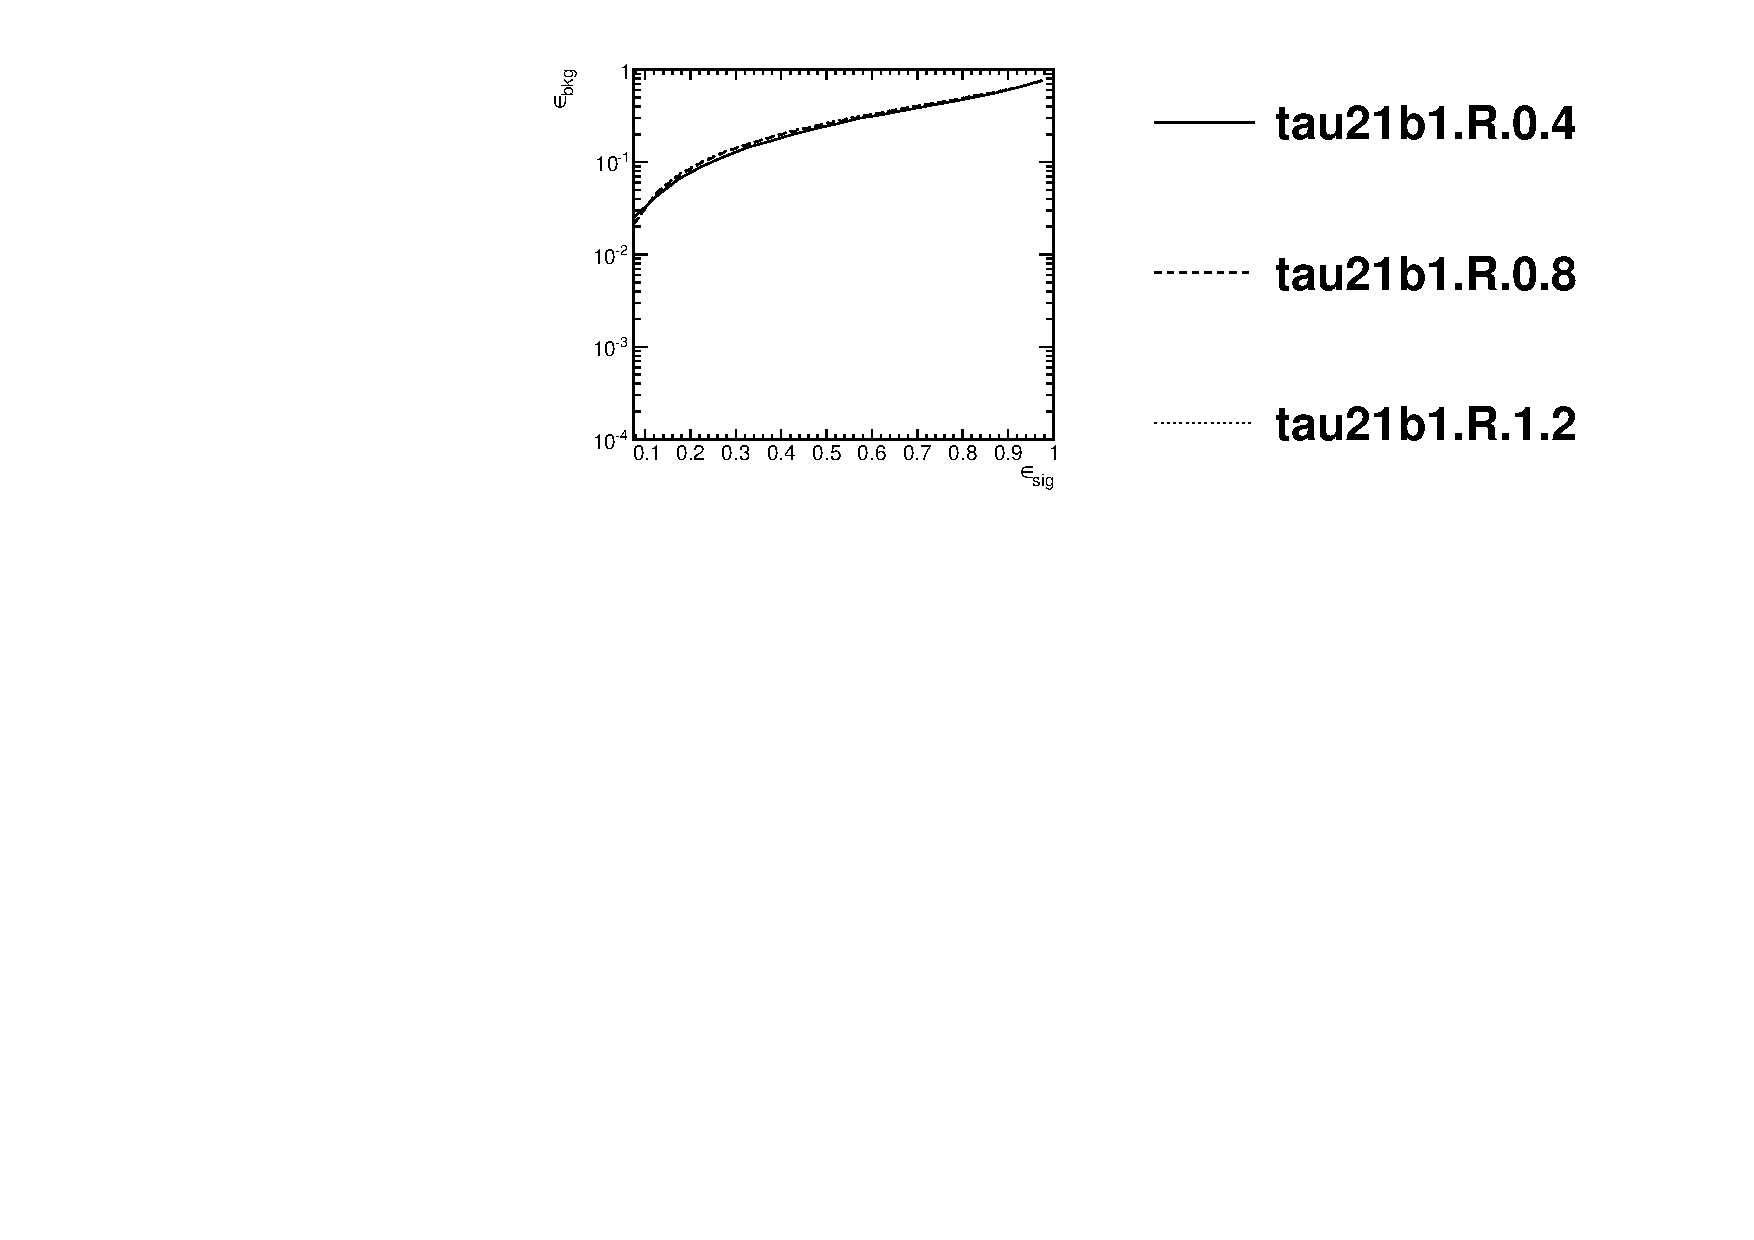
\includegraphics[width=0.48\textwidth]{./Figures/TTagging/single_variable/R_compare/Rocs_tau21b1_Rcompare.pdf}}
\subfigure[$\tau_{32}^{(\beta=1)}$]{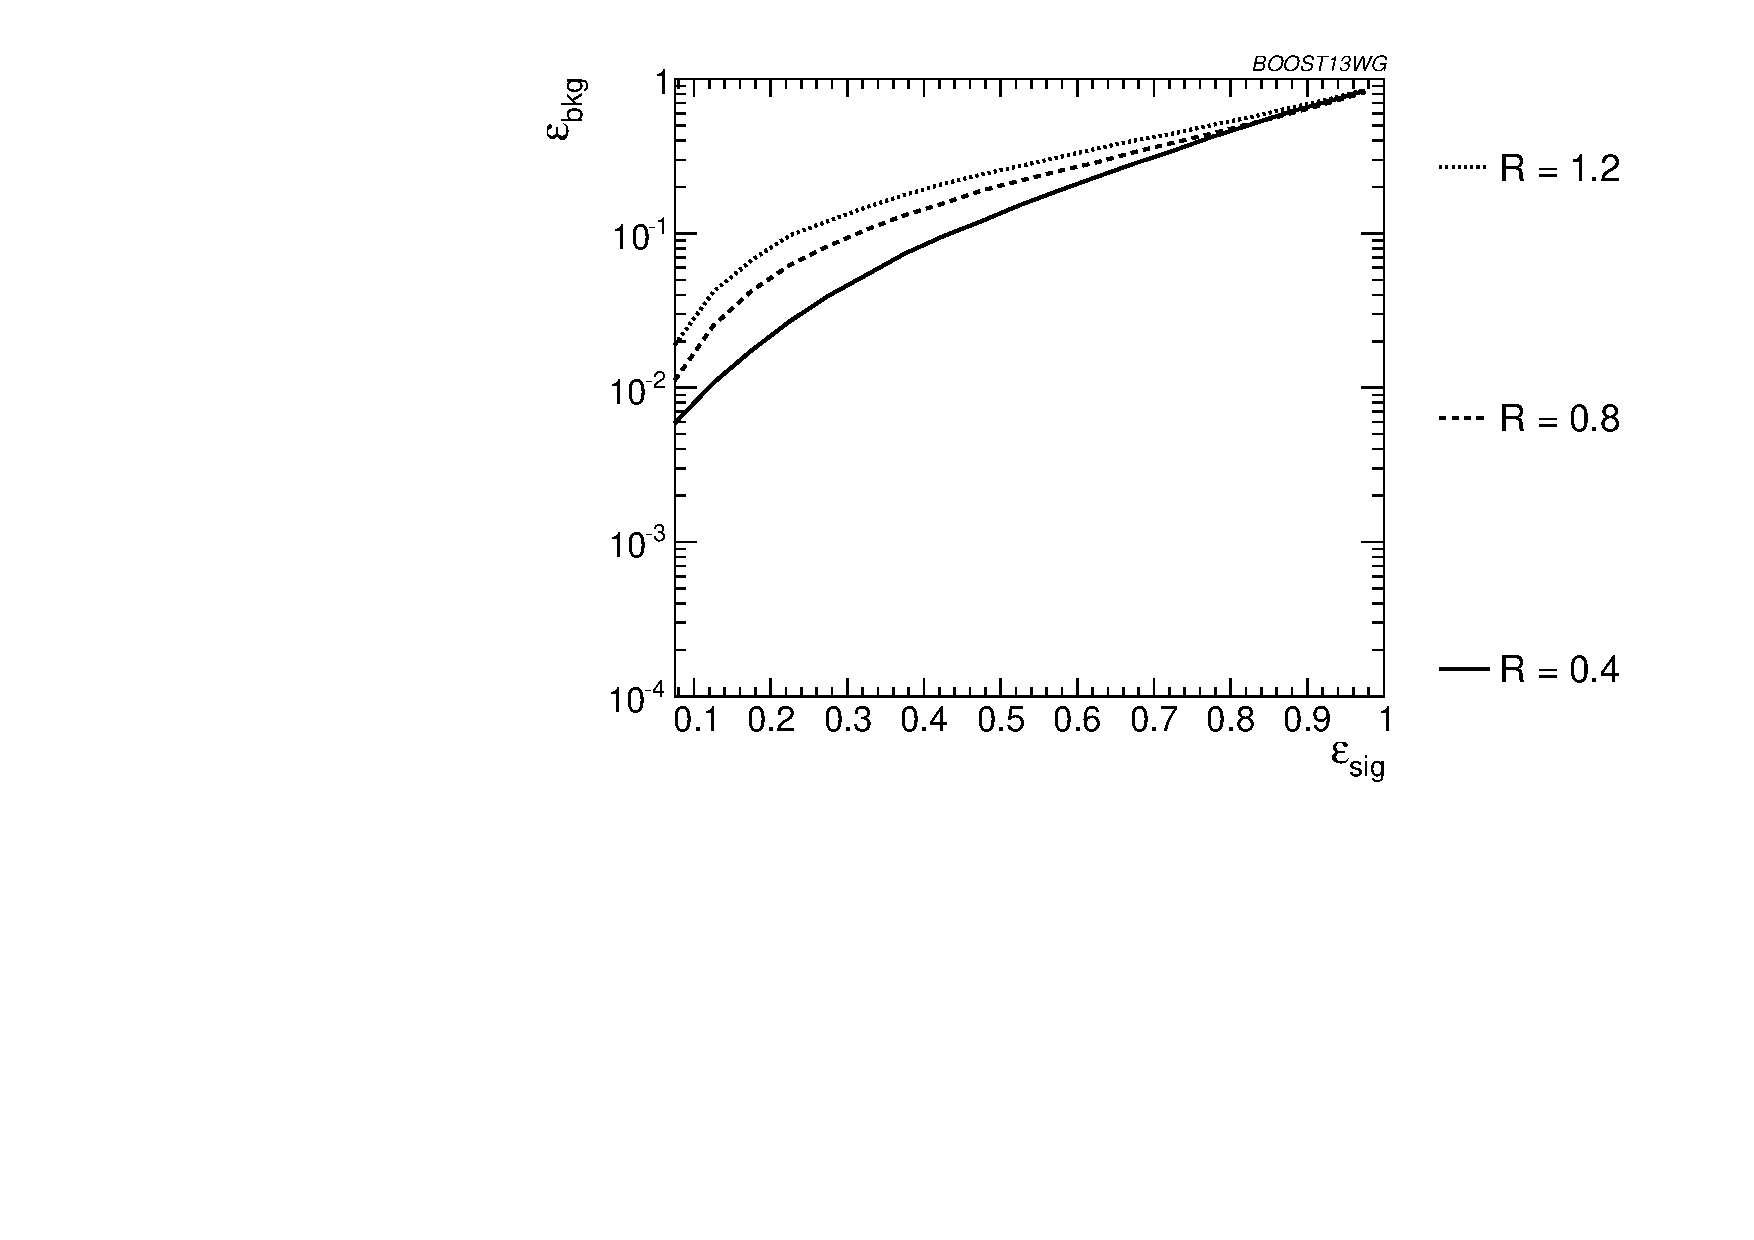
\includegraphics[width=0.48\textwidth]{./Figures/TTagging/single_variable/R_compare/Rocs_tau32b1_Rcompare.pdf}}
\subfigure[Qjet mass volatility]{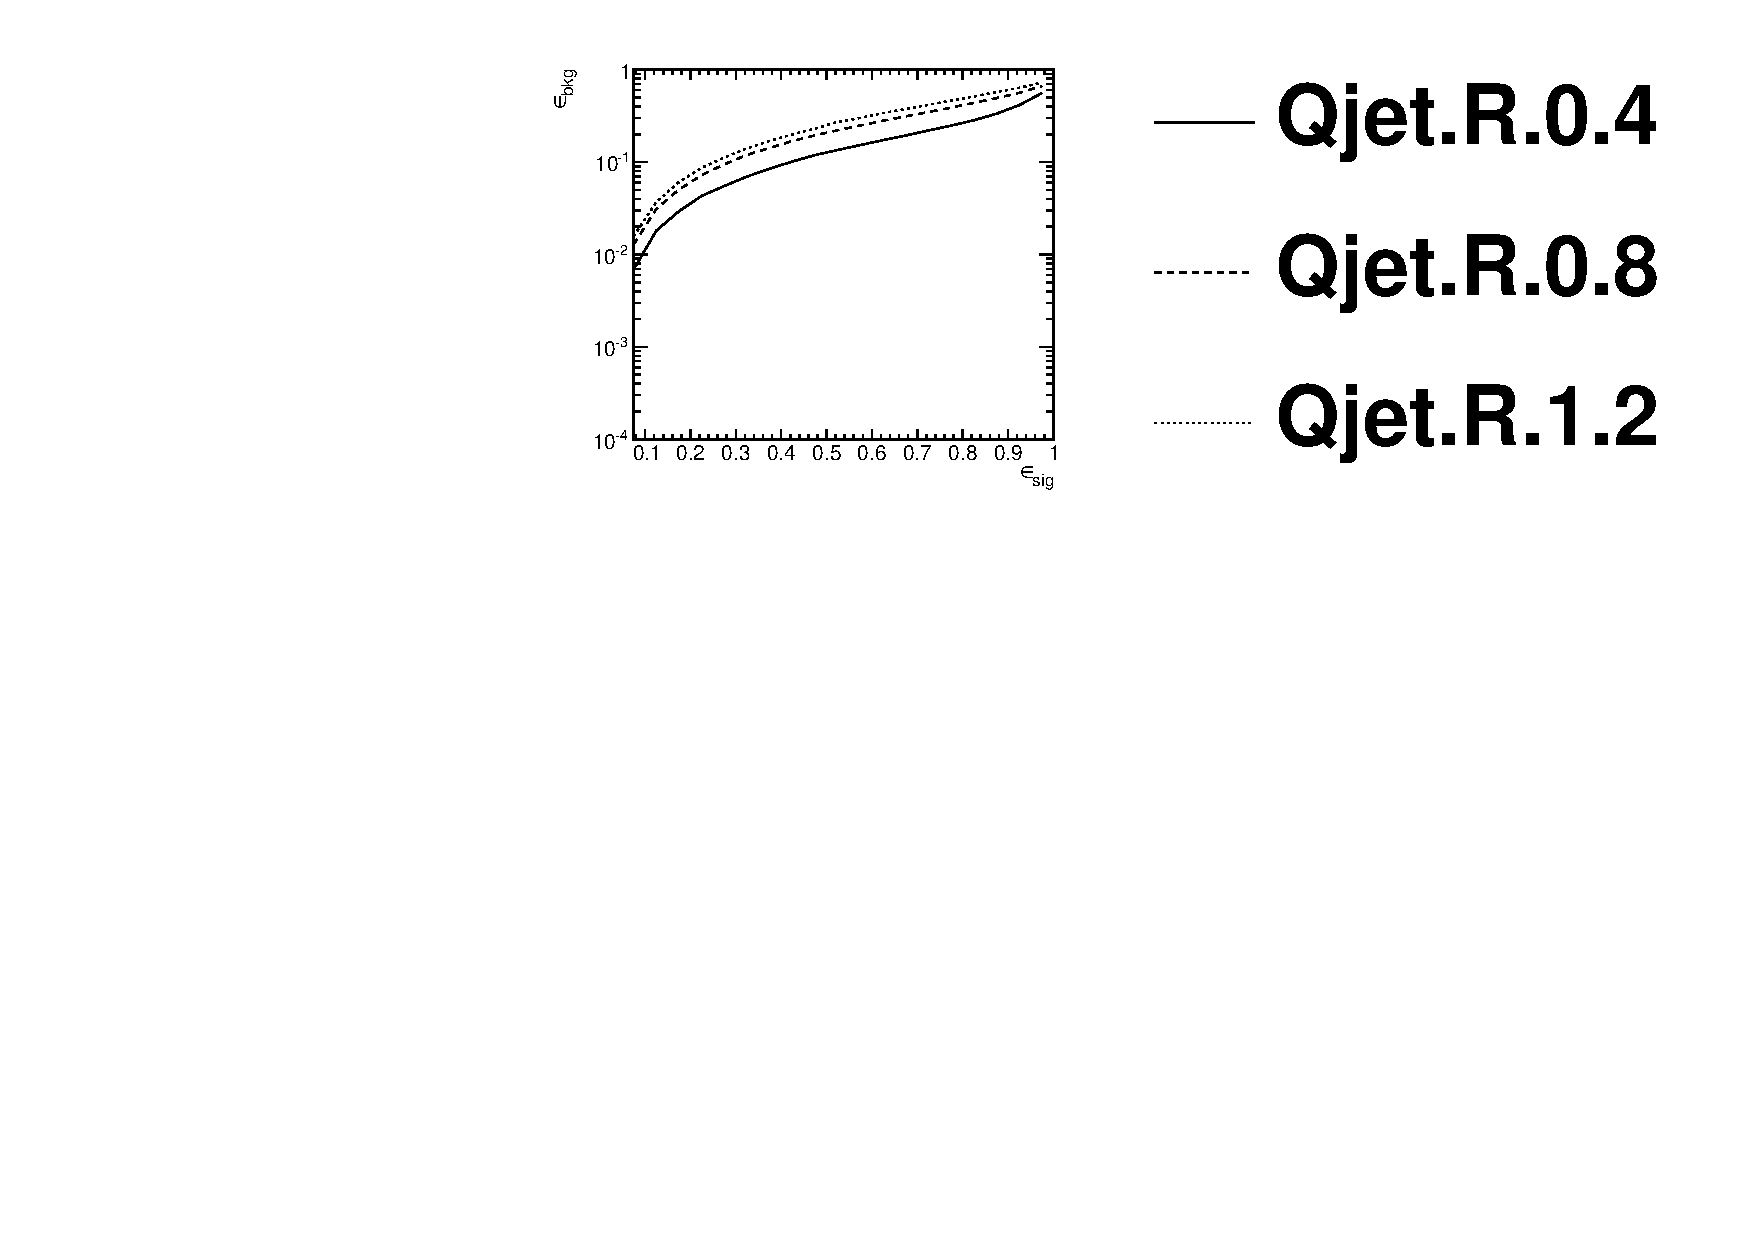
\includegraphics[width=0.48\textwidth]{./Figures/TTagging/single_variable/R_compare/Rocs_Qjet_Rcompare.pdf}}
\caption{Comparison of individual jet shape performance at different $R$ in the $\pt=1500-1600$ GeV bin.}
\label{fig:Rcomparison_singleshape_top}
\end{center}
\end{figure*}

\begin{figure*}
\begin{center}
\subfigure[HEPTopTagger $m_t$]{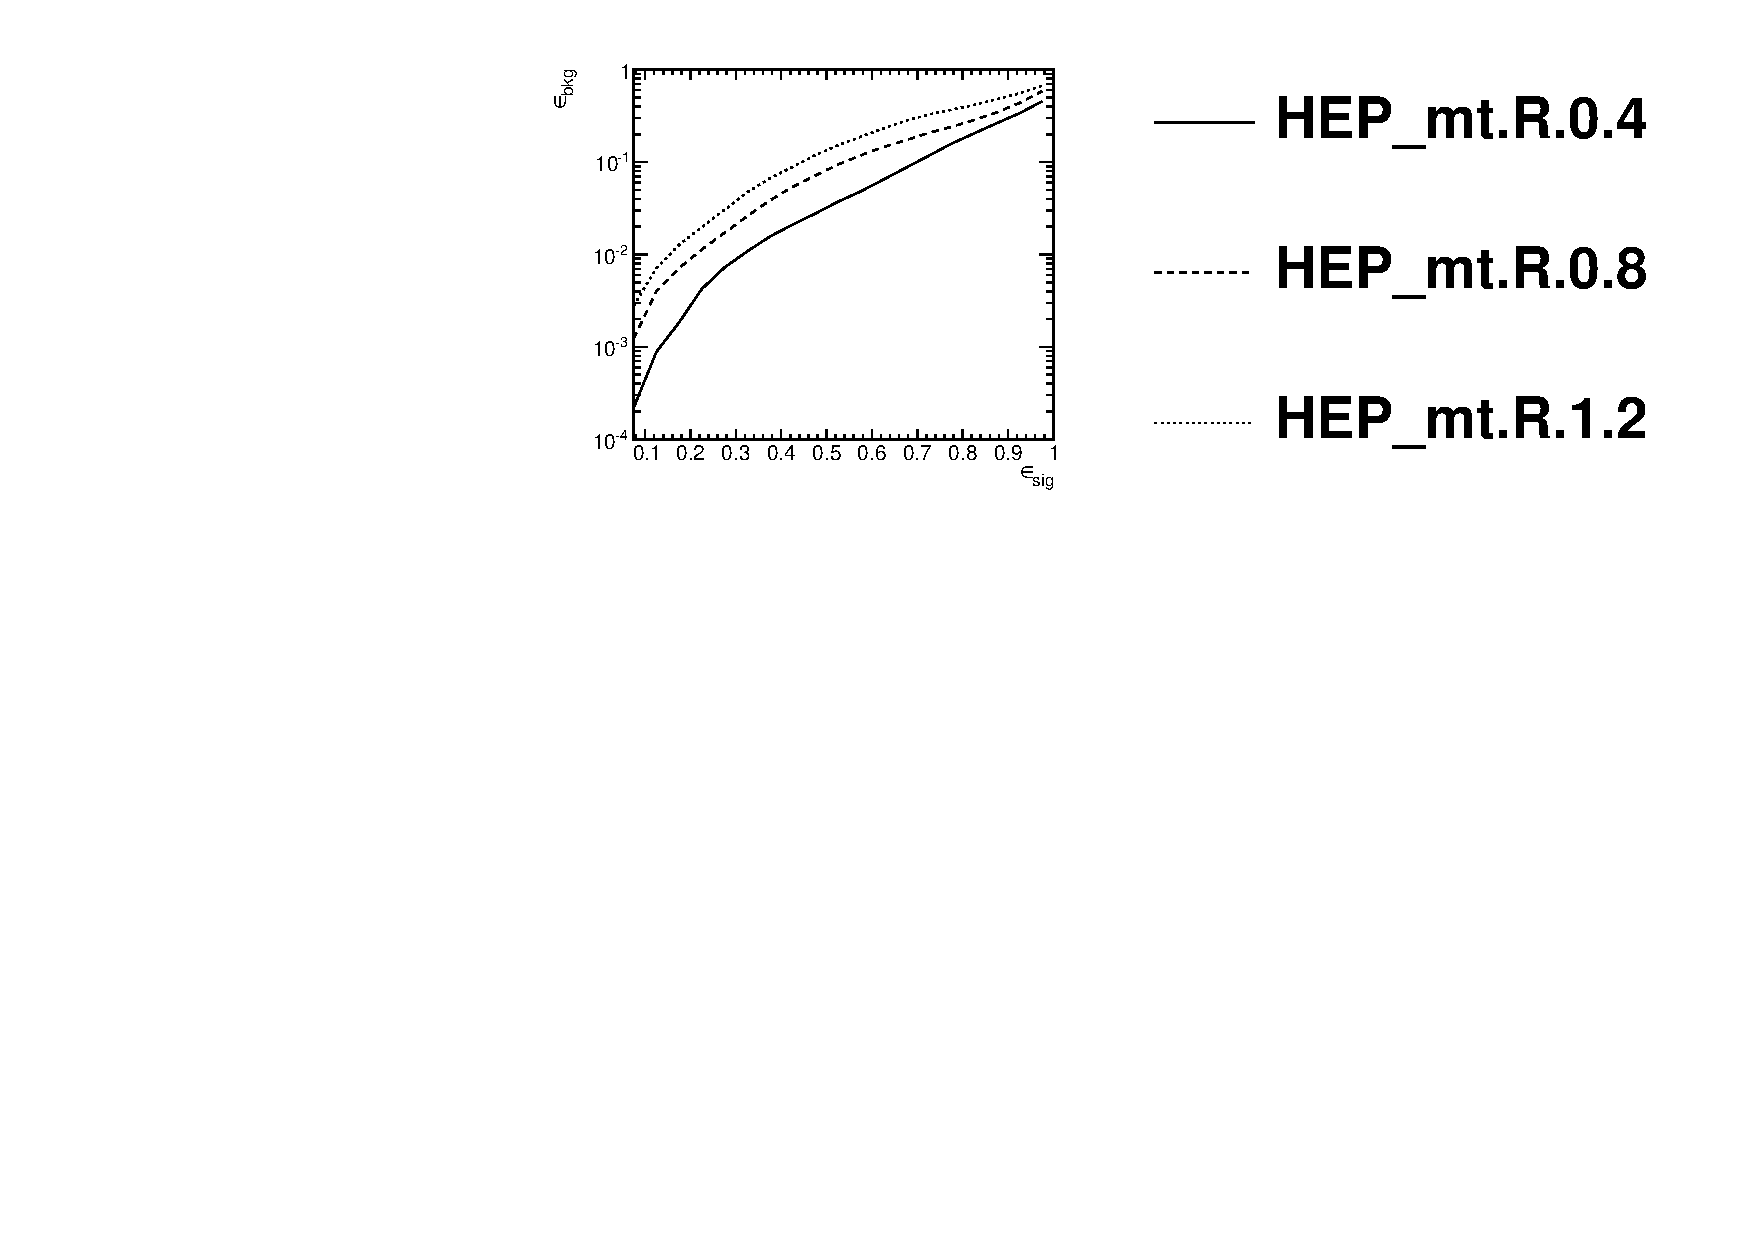
\includegraphics[width=0.48\textwidth]{./Figures/TTagging/single_variable/R_compare/Rocs_HEP_mt_Rcompare.pdf}}
\subfigure[Johns Hopkins Tagger $m_t$]{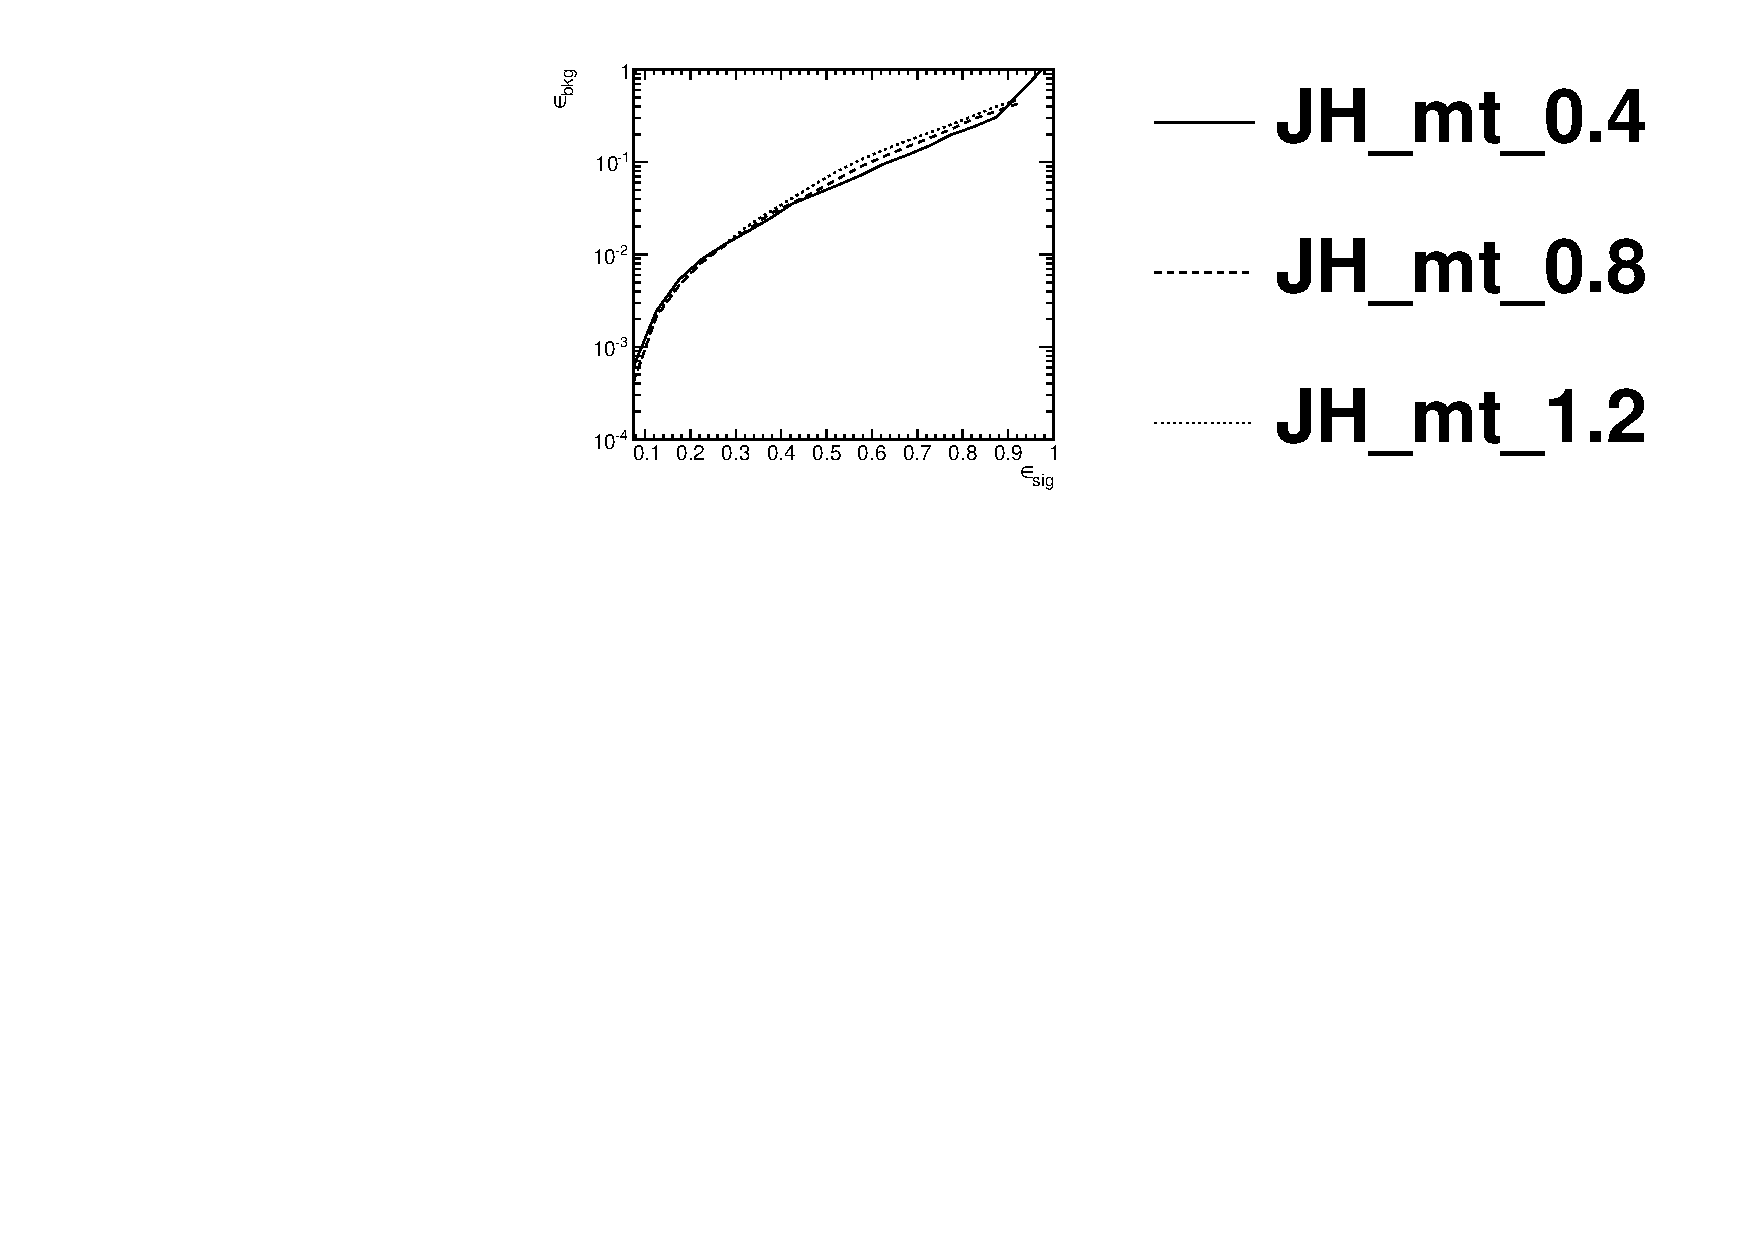
\includegraphics[width=0.48\textwidth]{./Figures/TTagging/single_variable/R_compare/Rocs_JH_mt_Rcompare.pdf}}
\subfigure[Pruning $m_t$]{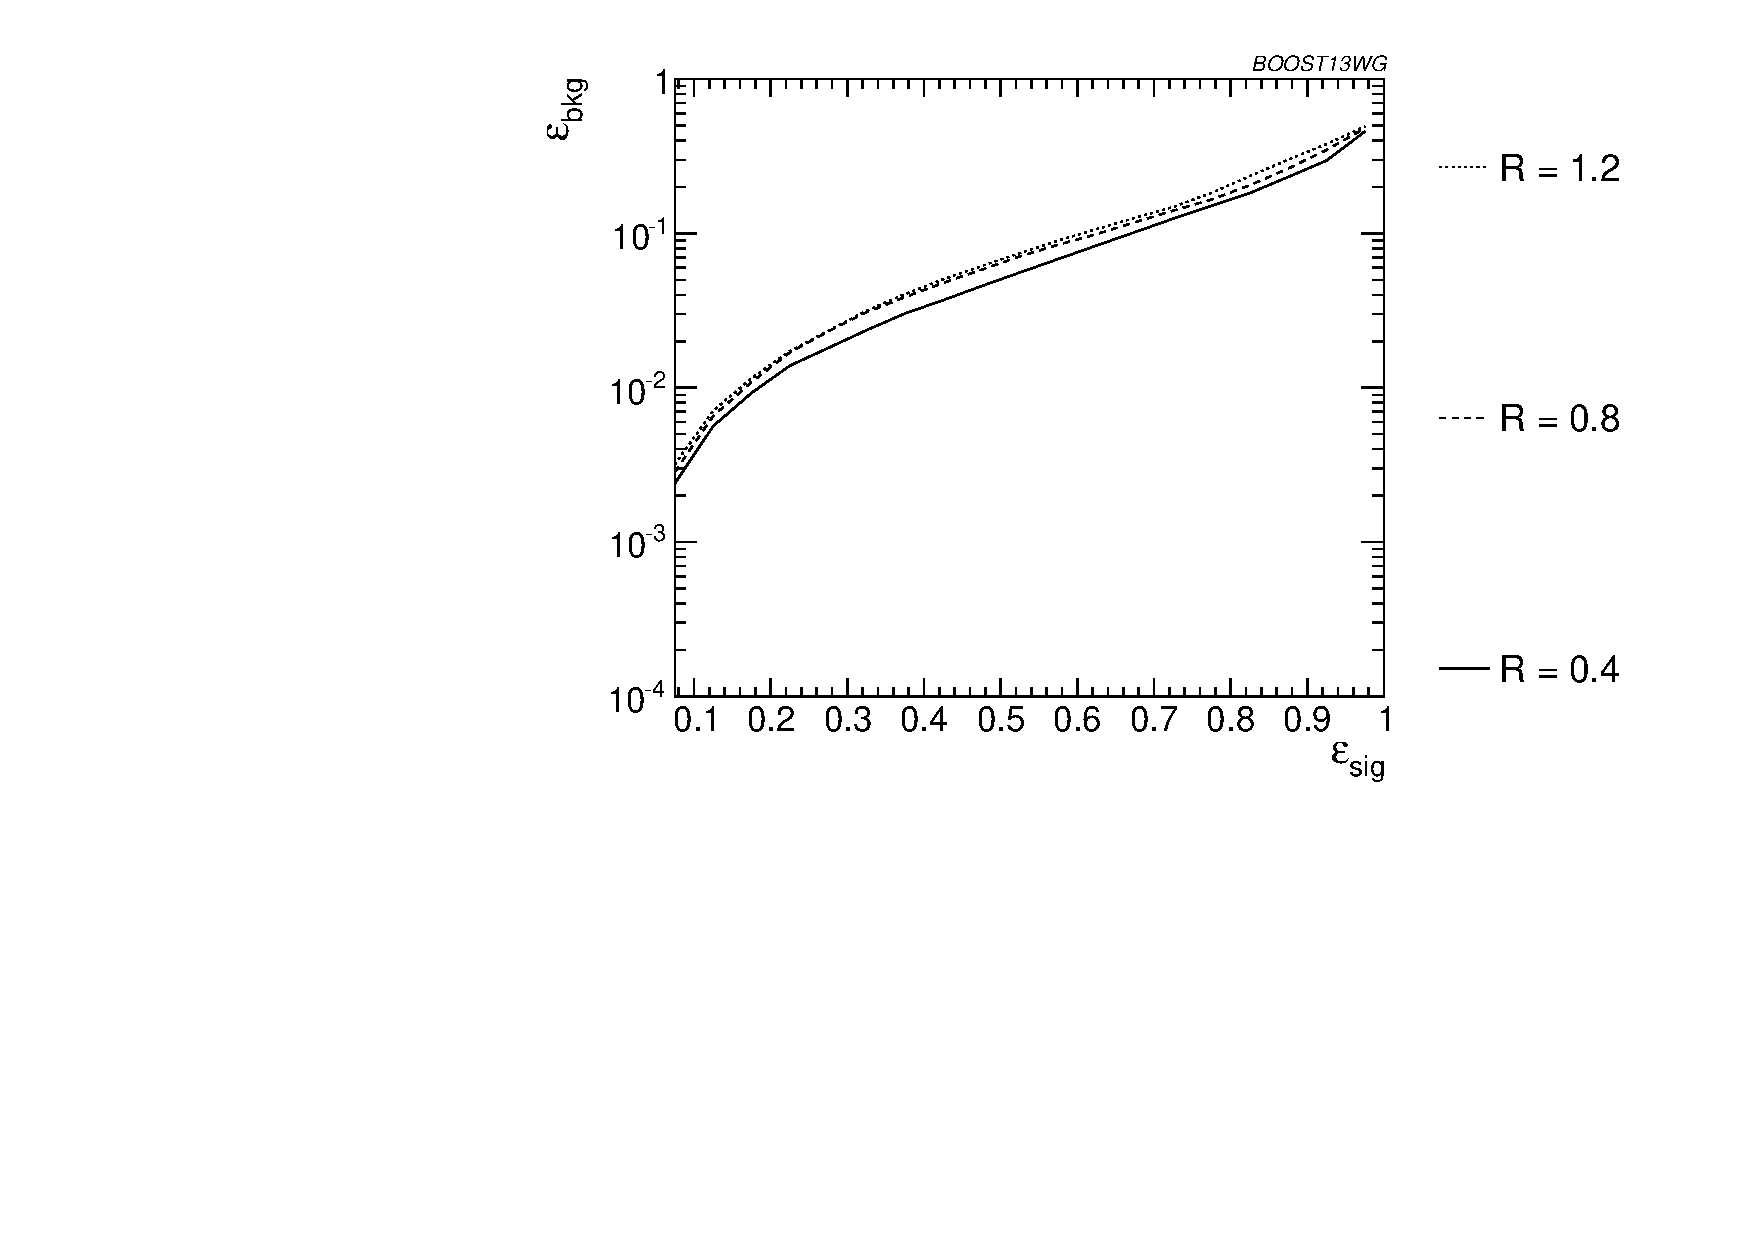
\includegraphics[width=0.48\textwidth]{./Figures/TTagging/single_variable/R_compare/Rocs_prune_Rcompare.pdf}}
\subfigure[Trimming $m_t$]{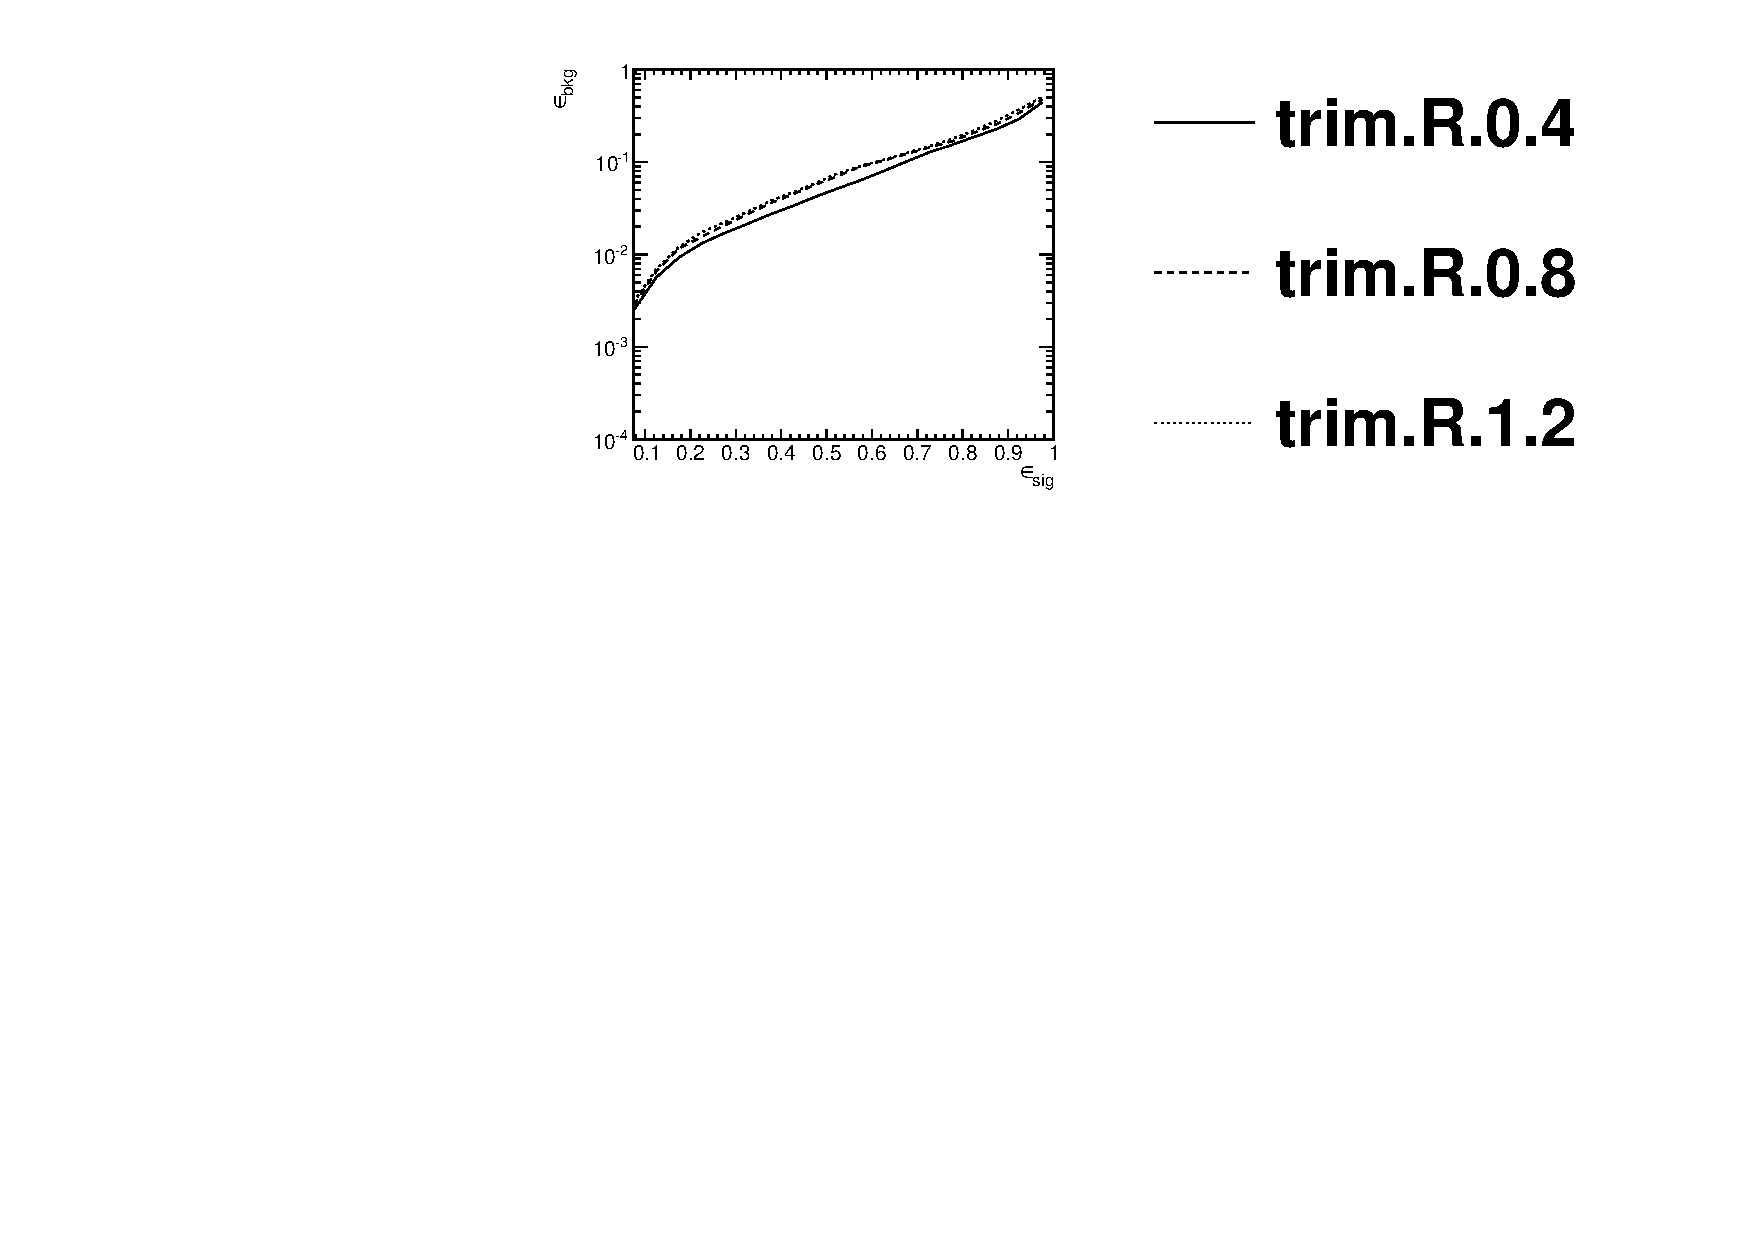
\includegraphics[width=0.48\textwidth]{./Figures/TTagging/single_variable/R_compare/Rocs_trim_Rcompare.pdf}}
\caption{Comparison of top mass performance of different taggers at different $R$ in the $\pt=1500-1600$ GeV bin.}
\label{fig:Rcomparison_singletopmass_top}
\end{center}
\end{figure*}

\begin{figure*}
\begin{center}
\subfigure[HEPTopTagger $m_W$]{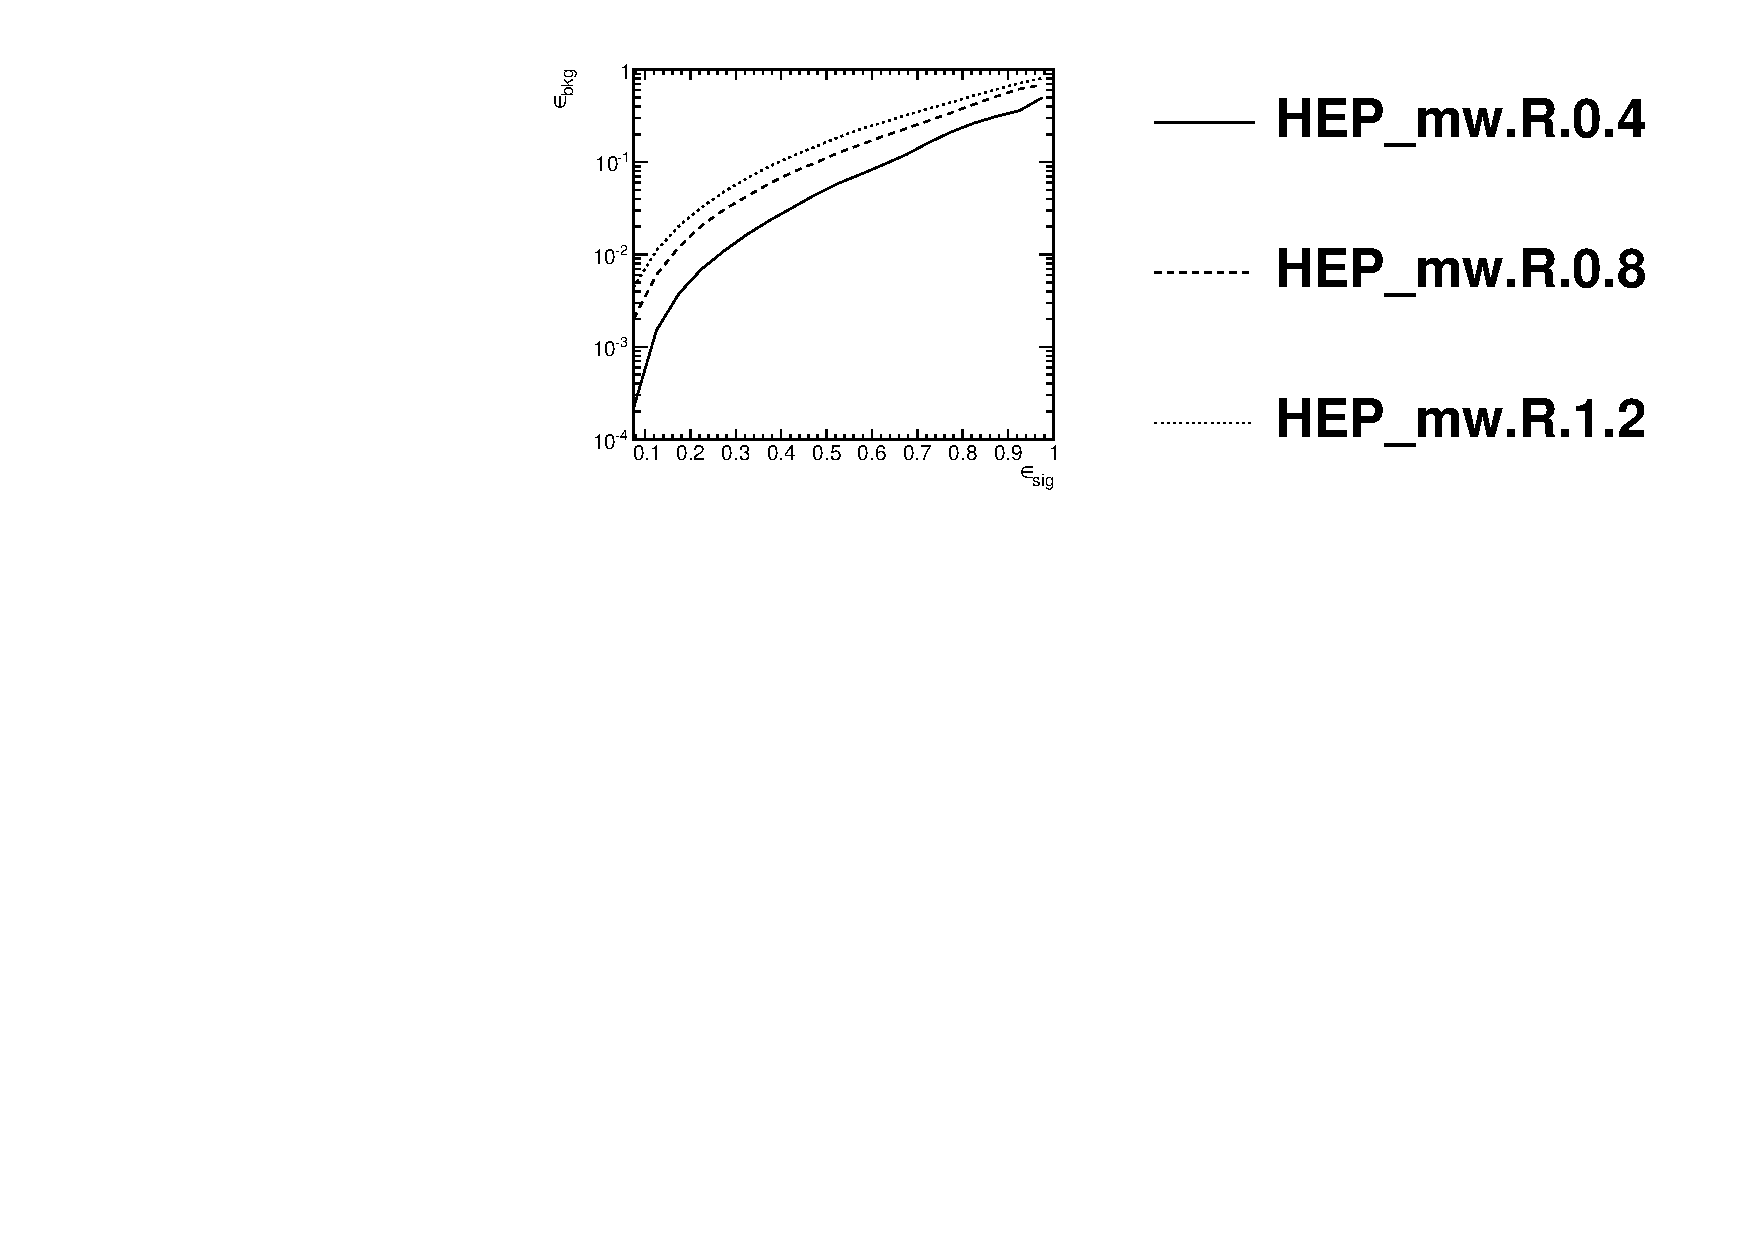
\includegraphics[width=0.48\textwidth]{./Figures/TTagging/single_variable/R_compare/Rocs_HEP_mw_Rcompare.pdf}}
\subfigure[Johns Hopkins Tagger $m_W$]{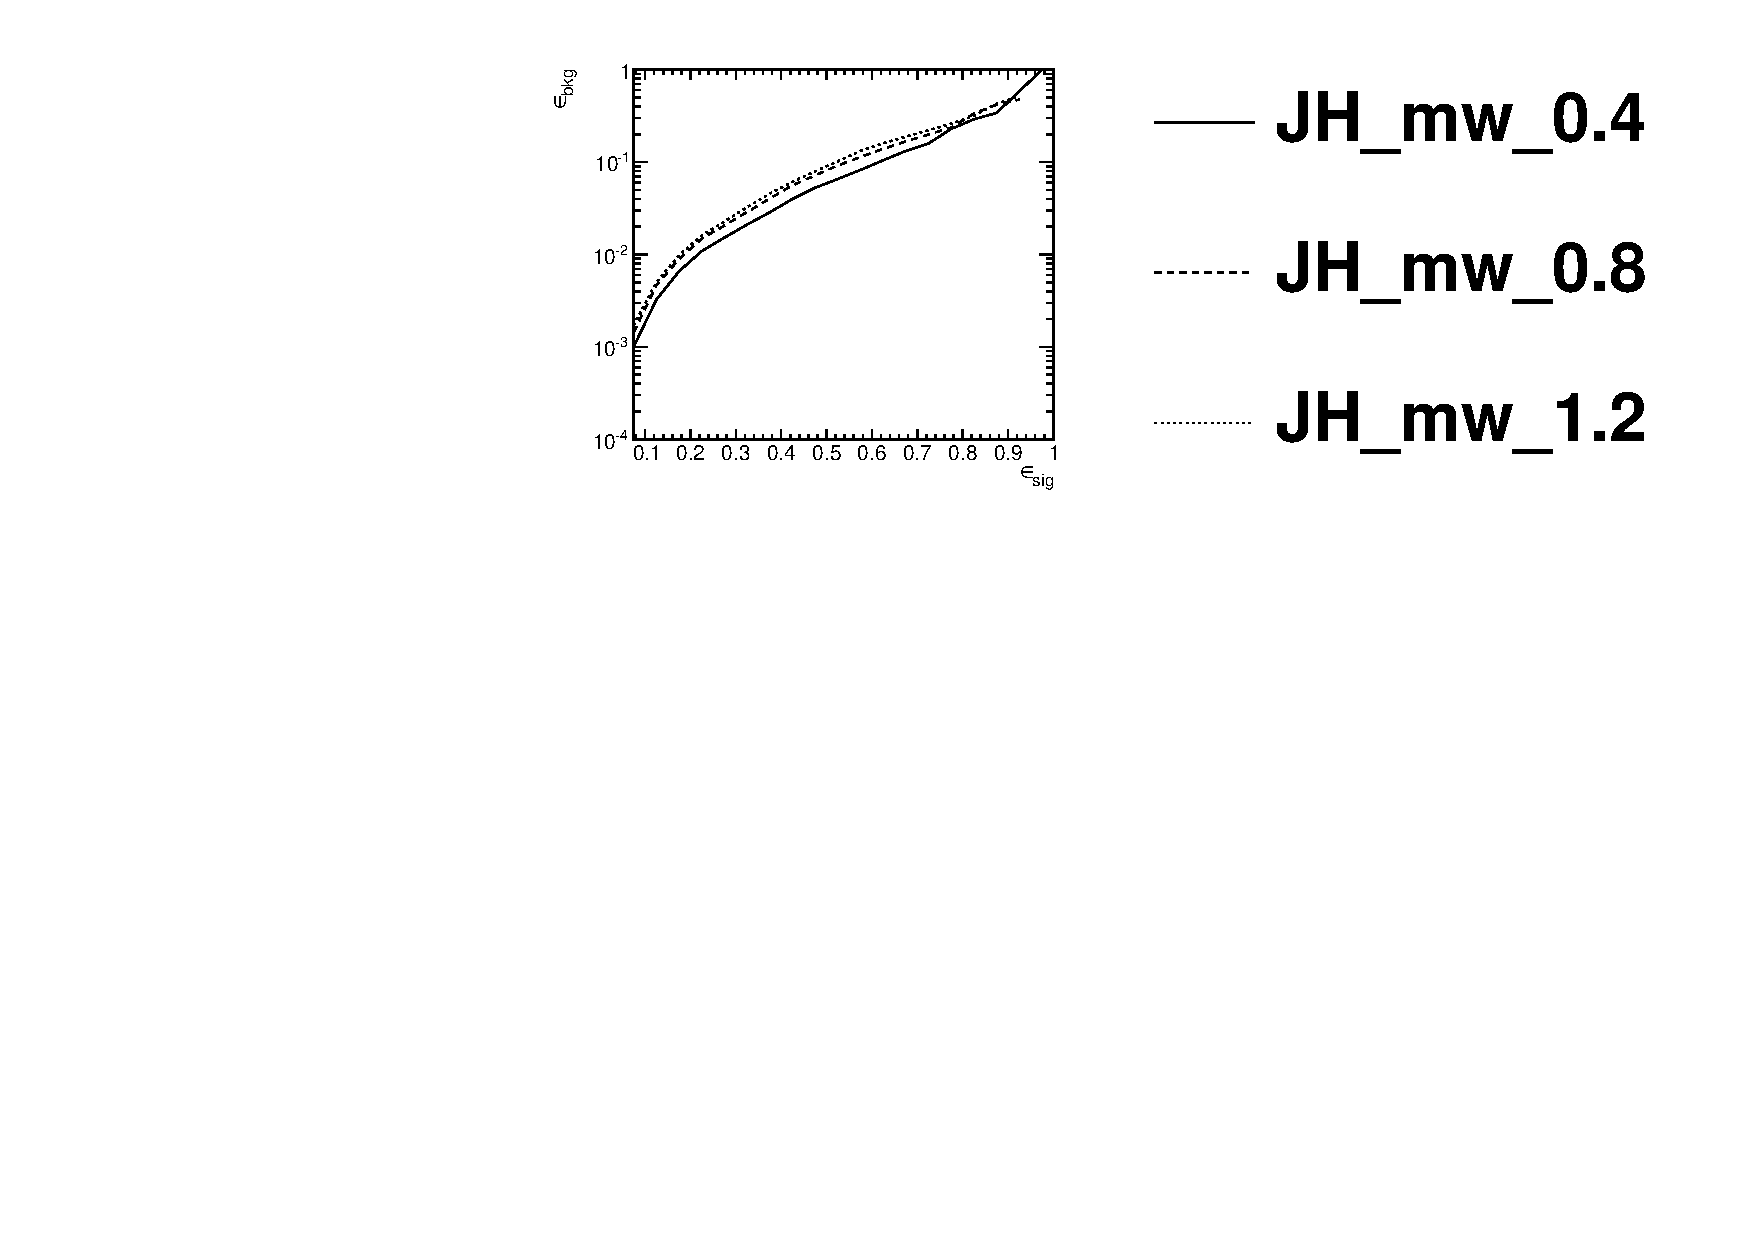
\includegraphics[width=0.48\textwidth]{./Figures/TTagging/single_variable/R_compare/Rocs_JH_mw_Rcompare.pdf}}
\subfigure[Pruning $m_W$]{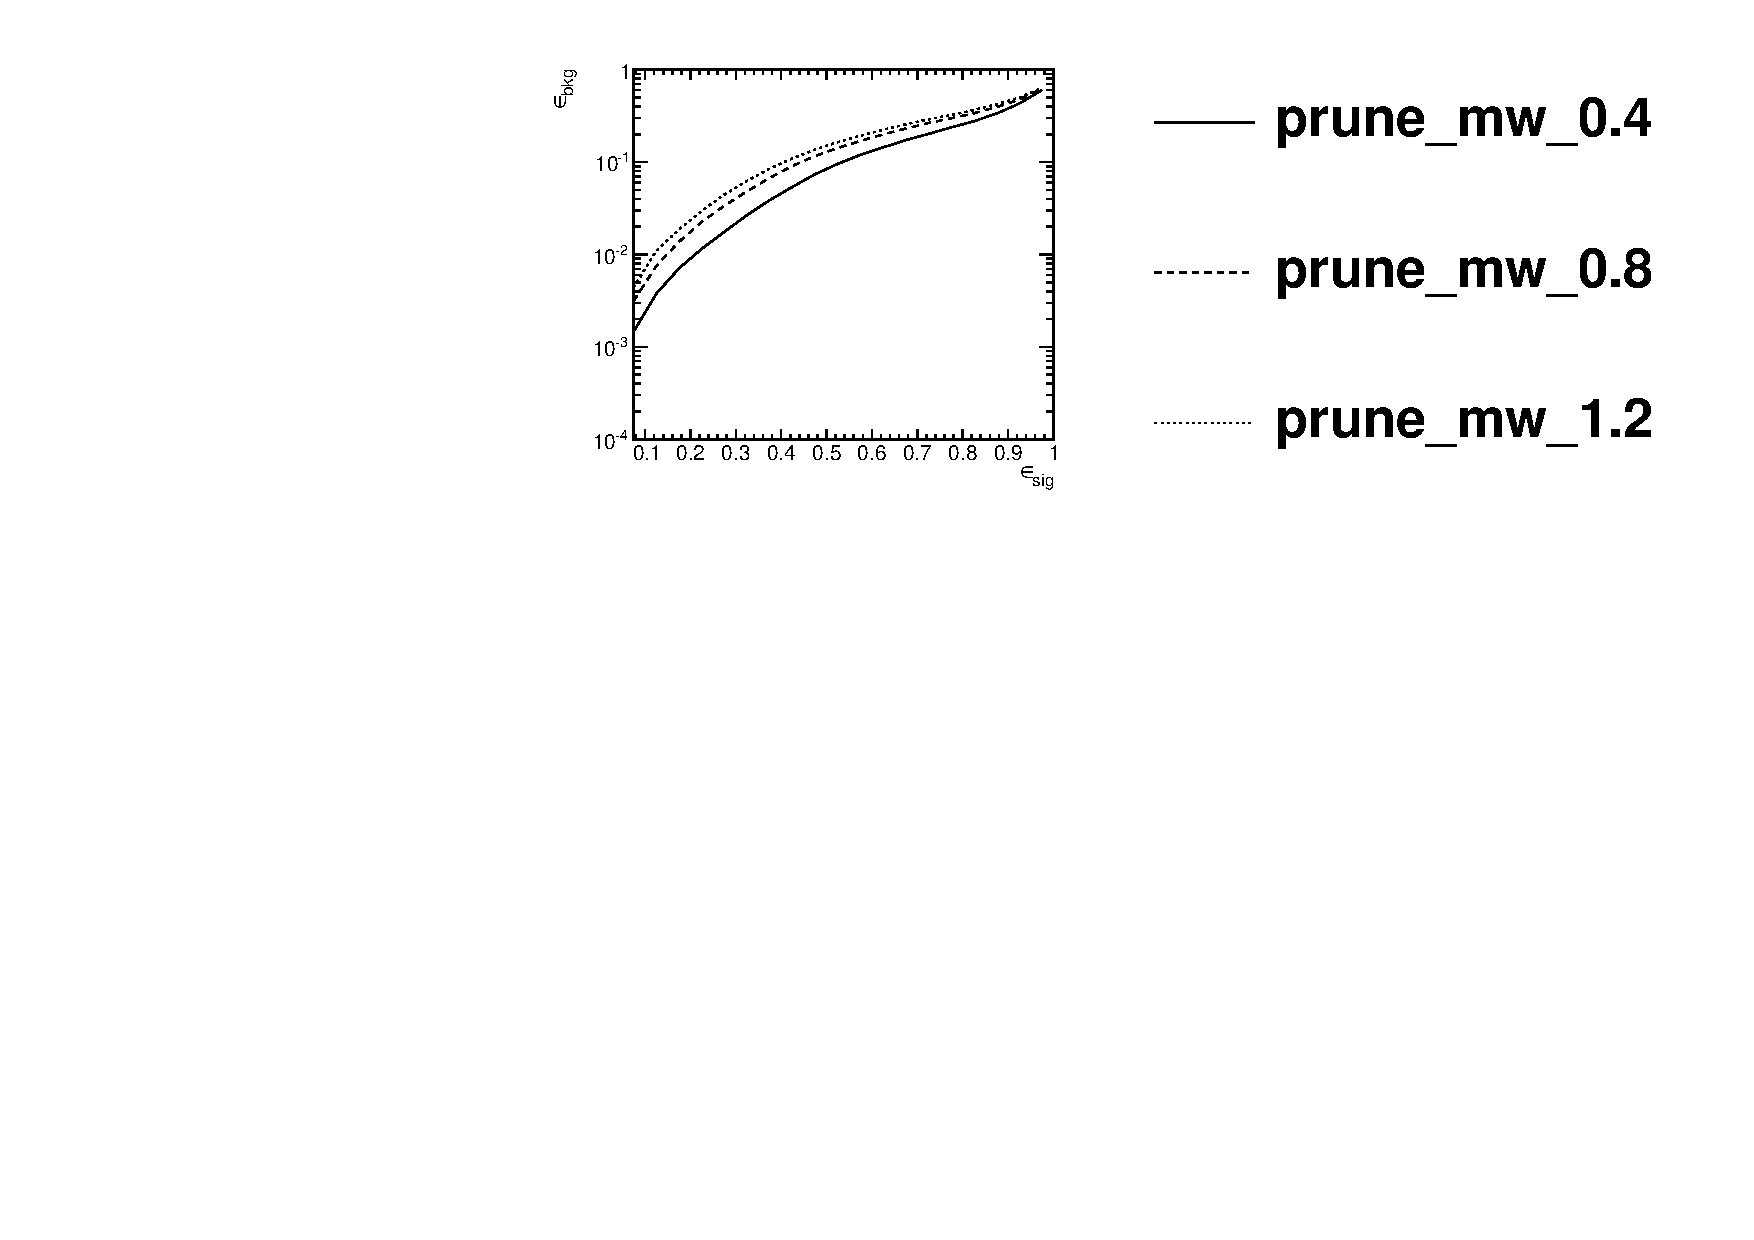
\includegraphics[width=0.48\textwidth]{./Figures/TTagging/single_variable/R_compare/Rocs_prune_mw_Rcompare.pdf}}
\subfigure[Trimming $m_W$]{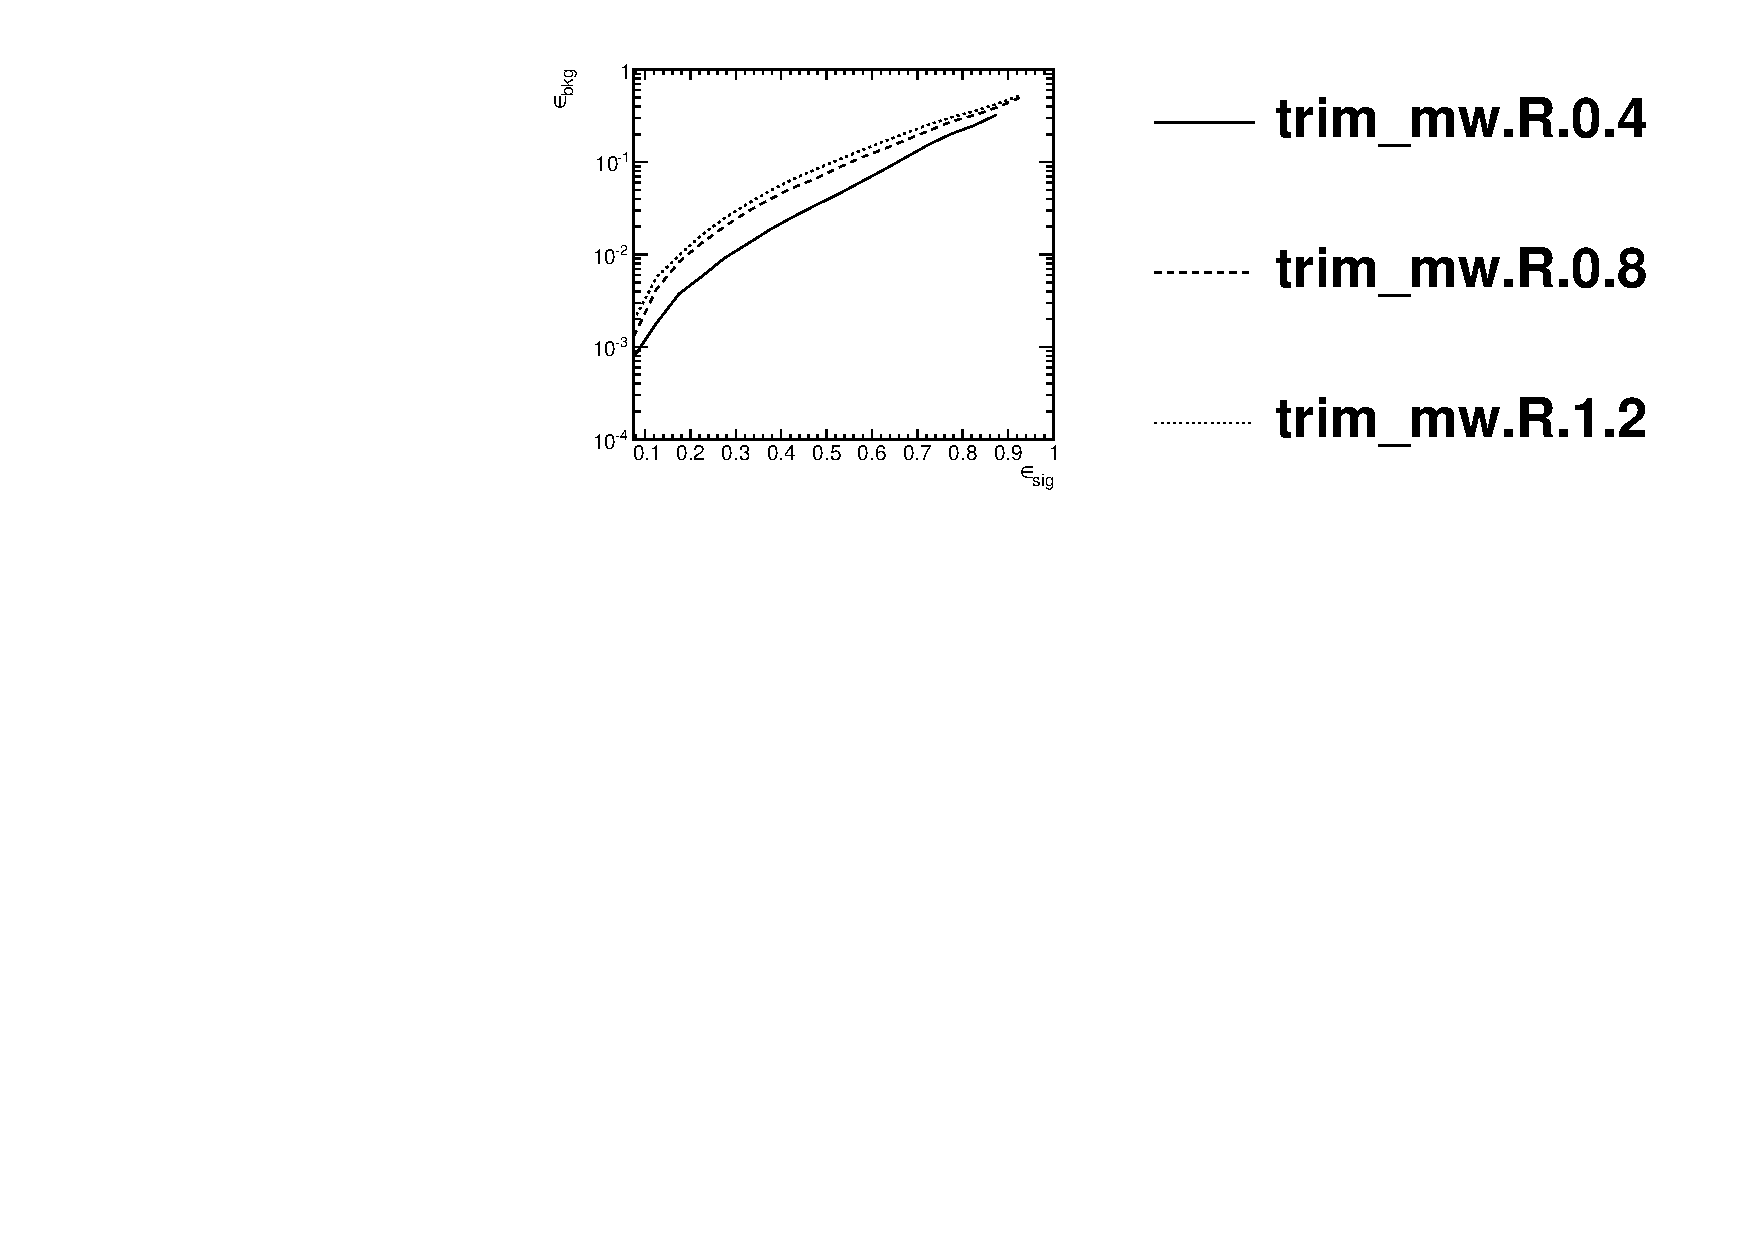
\includegraphics[width=0.48\textwidth]{./Figures/TTagging/single_variable/R_compare/Rocs_trim_mw_Rcompare.pdf}}
\caption{Comparison of $W$ mass performance of different taggers at different $R$ in the $\pt=1500-1600$ GeV bin.}
\label{fig:Rcomparison_singlewmass_top}
\end{center}
\end{figure*}


\subsection{Performance of multivariable combinations}


\begin{figure*}
\begin{center}
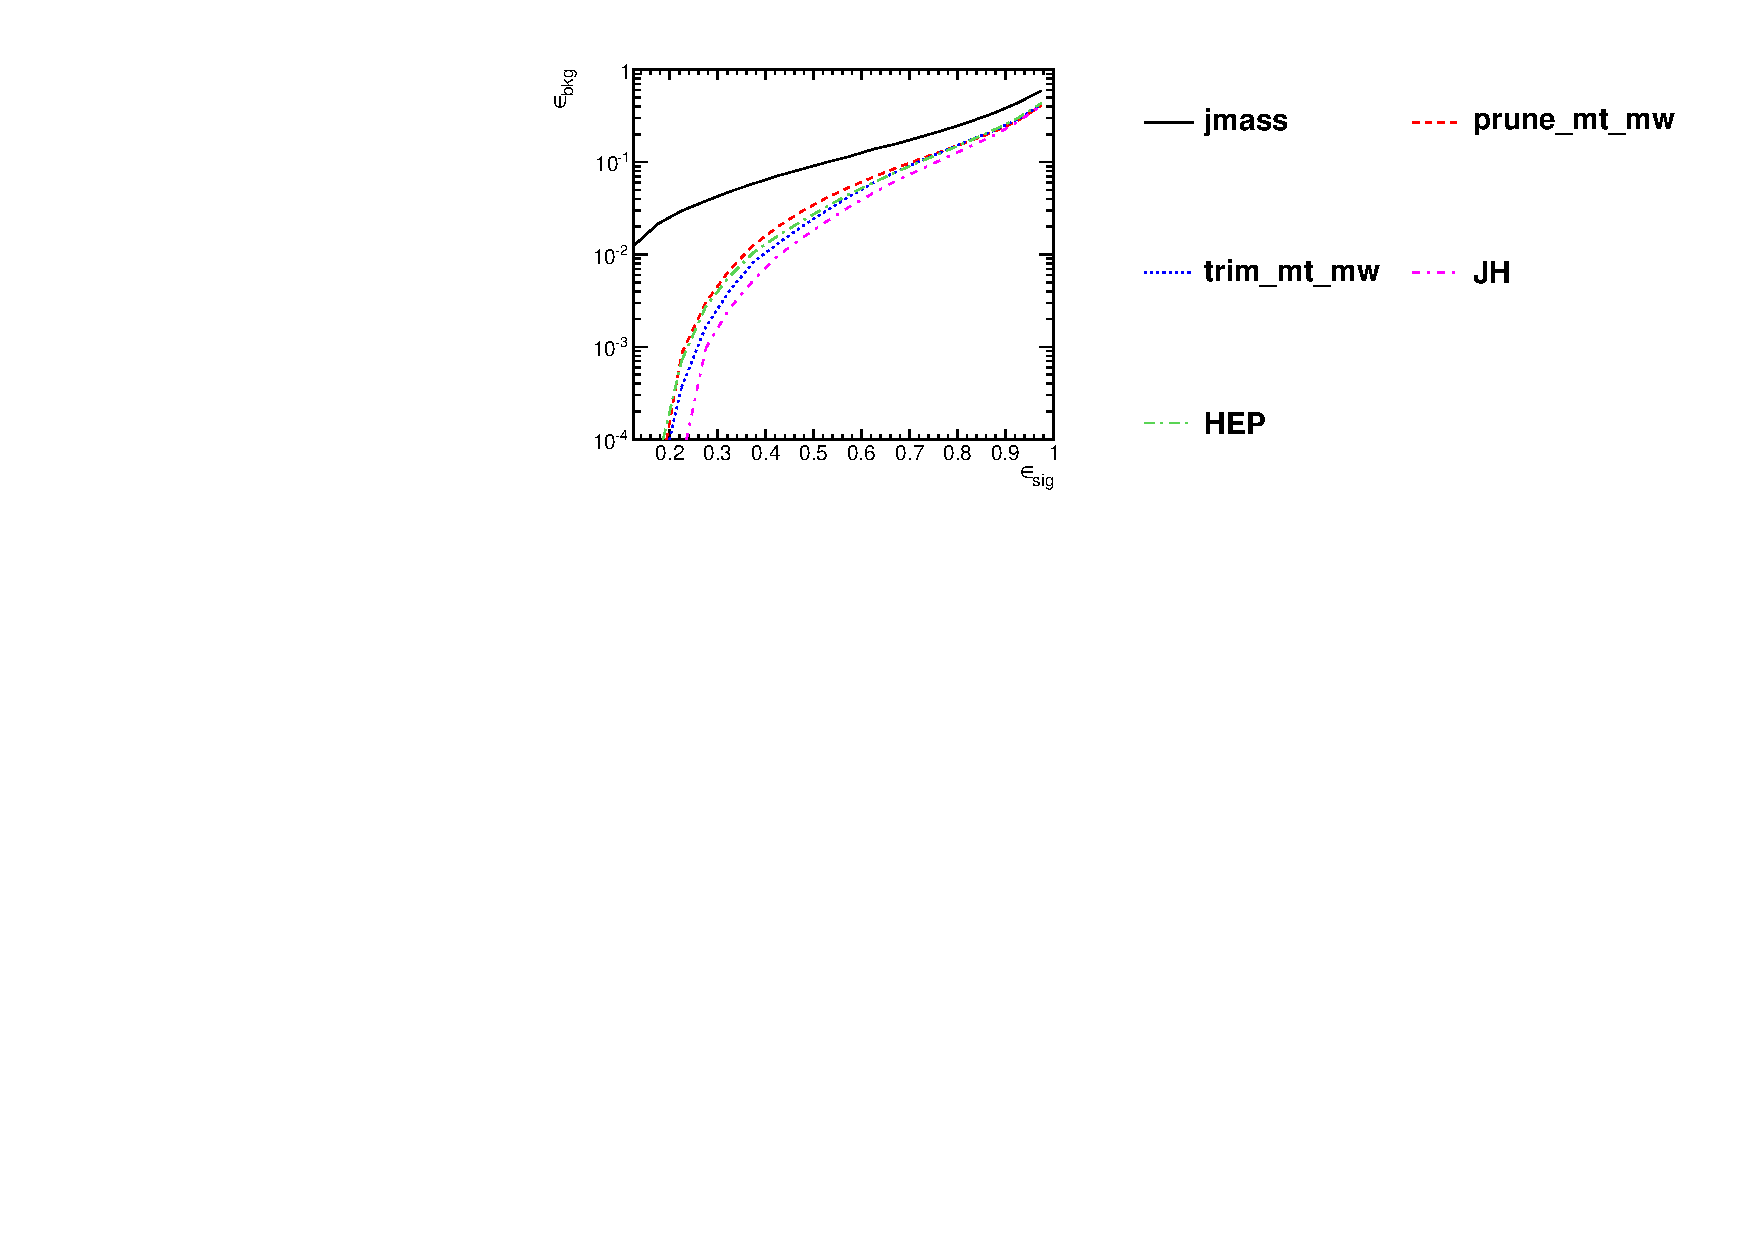
\includegraphics[width=0.7\textwidth]{./Figures/TTagging/multi_variable/pT.1TeV.R.0.8/Rocs_tagger_groom.pdf}
\caption{Comparison of BDT combinations of each tagger output in the \pt 1000-1100 GeV bin using the anti-\kT R=0.8 algorithm.}
\label{fig:pt1000_taggers_AKt_R08}
\end{center}
\end{figure*}


\begin{figure*}
\begin{center}
\subfigure[HEPTopTagger]{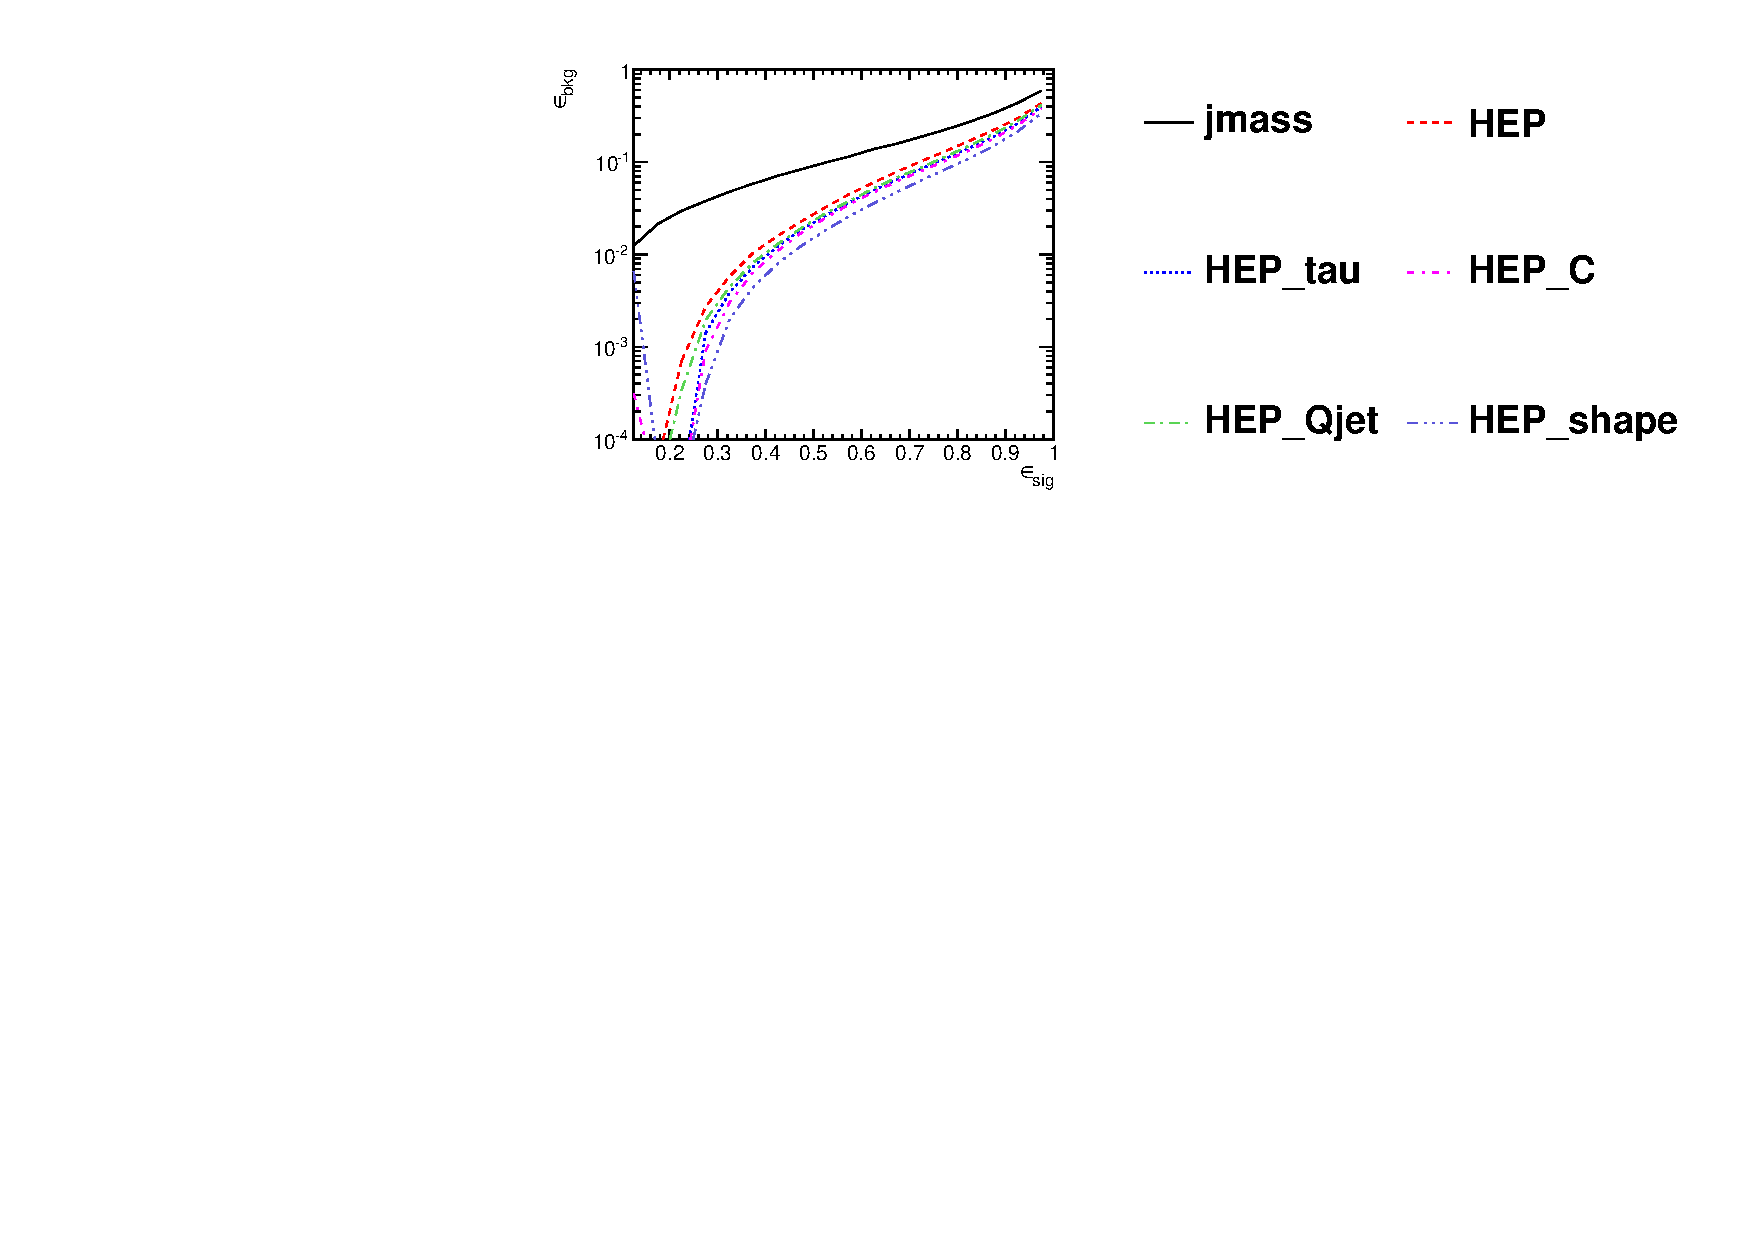
\includegraphics[width=0.48\textwidth]{./Figures/TTagging/multi_variable/pT.1TeV.R.0.8/Rocs_HEP.pdf}}
\subfigure[Johns Hopkins Tagger]{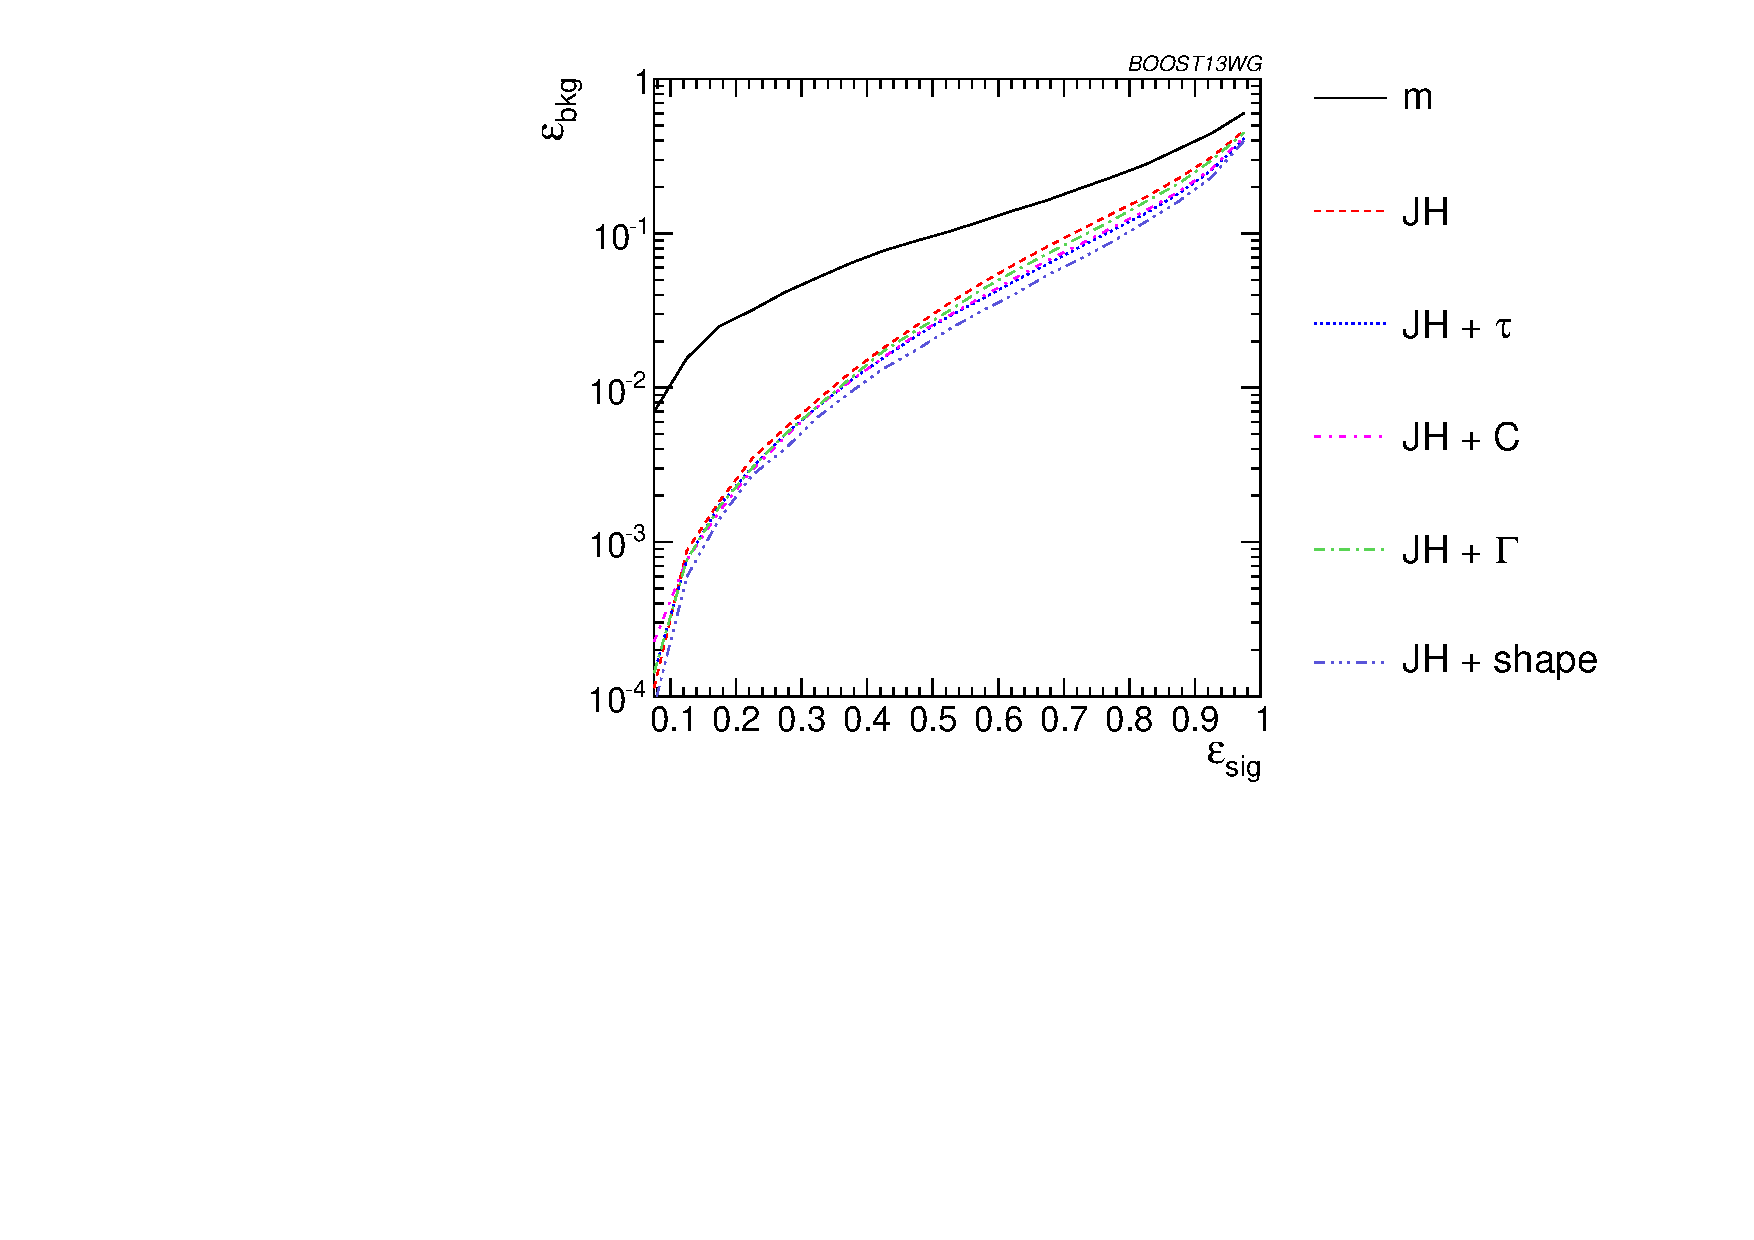
\includegraphics[width=0.48\textwidth]{./Figures/TTagging/multi_variable/pT.1TeV.R.0.8/Rocs_JH.pdf}}
\subfigure[Pruning]{\includegraphics[width=0.48\textwidth]{./Figures/TTagging/multi_variable/pT.1TeV.R.0.8/Rocs_prune.pdf}}
\subfigure[Trimming]{\includegraphics[width=0.48\textwidth]{./Figures/TTagging/multi_variable/pT.1TeV.R.0.8/Rocs_trim.pdf}}
\subfigure[HEP+JH comparison]{\includegraphics[width=0.48\textwidth]{./Figures/TTagging/multi_variable/pT.1TeV.R.0.8/Rocs_tagger_shape.pdf}}
\subfigure[Grooming comparison]{\includegraphics[width=0.48\textwidth]{./Figures/TTagging/multi_variable/pT.1TeV.R.0.8/Rocs_groom_shape.pdf}}
\subfigure[Comparison of Tagger+Shape]{\includegraphics[width=0.48\textwidth]{./Figures/TTagging/multi_variable/pT.1TeV.R.0.8/Rocs_optimum.pdf}}
\caption{The BDT combinations in the \pt 1000-1100 GeV bin using the anti-\kT R=0.8 algorithm.}
\label{fig:pt1000_taggers_AKt_R08}
\end{center}
\end{figure*}

\clearpage


\subsubsection{$\pt$ comparison}

\begin{figure*}
\begin{center}
\subfigure[HEPTopTagger]{\includegraphics[width=0.48\textwidth]{./Figures/TTagging/multi_variable/pT_compare/Rocs_HEP_pTcompare.pdf}}
\subfigure[Johns Hopkins Tagger]{\includegraphics[width=0.48\textwidth]{./Figures/TTagging/multi_variable/pT_compare/Rocs_JH_pTcompare.pdf}}
\subfigure[JH + HEP taggers]{\includegraphics[width=0.48\textwidth]{./Figures/TTagging/multi_variable/pT_compare/Rocs_HEP_JH_pTcompare.pdf}}
\subfigure[Trimming]{\includegraphics[width=0.48\textwidth]{./Figures/TTagging/multi_variable/pT_compare/Rocs_trim_mt_mw_pTcompare.pdf}}
\subfigure[Pruning]{\includegraphics[width=0.48\textwidth]{./Figures/TTagging/multi_variable/pT_compare/Rocs_prune_mt_mw_pTcompare.pdf}}
\caption{Comparison of BDT combination of tagger performance at different \pt using the anti-\kT R=0.8 algorithm.}
\label{fig:ptcomparison_top}
\end{center}
\end{figure*}

\begin{figure*}
\begin{center}
\subfigure[JH+$C_2^{(\beta=1)}$+$C_3^{(\beta=1)}$]{\includegraphics[width=0.48\textwidth]{./Figures/TTagging/multi_variable/pT_compare/Rocs_JH_C_pTcompare.pdf}}
\subfigure[JH+$\tau_{21}^{(\beta=1)}$+$\tau_{32}^{(\beta=1)}$]{\includegraphics[width=0.48\textwidth]{./Figures/TTagging/multi_variable/pT_compare/Rocs_JH_tau_pTcompare.pdf}}
\subfigure[JH + Qjet mass volatility]{\includegraphics[width=0.48\textwidth]{./Figures/TTagging/multi_variable/pT_compare/Rocs_JH_Qjet_pTcompare.pdf}}
\subfigure[JH + all]{\includegraphics[width=0.48\textwidth]{./Figures/TTagging/multi_variable/pT_compare/Rocs_JH_shape_pTcompare.pdf}}
\caption{Comparison of BDT combination of JH tagger + shape at different \pt using the anti-\kT R=0.8 algorithm.}
\label{fig:ptcomparison_JH_shape}
\end{center}
\end{figure*}

\begin{figure*}
\begin{center}
\subfigure[HEP+$C_2^{(\beta=1)}$+$C_3^{(\beta=1)}$]{\includegraphics[width=0.48\textwidth]{./Figures/TTagging/multi_variable/pT_compare/Rocs_HEP_C_pTcompare.pdf}}
\subfigure[HEP+$\tau_{21}^{(\beta=1)}$+$\tau_{32}^{(\beta=1)}$]{\includegraphics[width=0.48\textwidth]{./Figures/TTagging/multi_variable/pT_compare/Rocs_HEP_tau_pTcompare.pdf}}
\subfigure[HEP + Qjet mass volatility]{\includegraphics[width=0.48\textwidth]{./Figures/TTagging/multi_variable/pT_compare/Rocs_HEP_Qjet_pTcompare.pdf}}
\subfigure[HEP + all]{\includegraphics[width=0.48\textwidth]{./Figures/TTagging/multi_variable/pT_compare/Rocs_HEP_shape_pTcompare.pdf}}
\caption{Comparison of BDT combination of HEP tagger + shape at different \pt using the anti-\kT R=0.8 algorithm.}
\label{fig:ptcomparison_HEP_shape}
\end{center}
\end{figure*}

\begin{figure*}
\begin{center}
\subfigure[trim $m_t$+$m_W$+$C_2^{(\beta=1)}$+$C_3^{(\beta=1)}$]{\includegraphics[width=0.48\textwidth]{./Figures/TTagging/multi_variable/pT_compare/Rocs_trim_mt_mw_C_pTcompare.pdf}}
\subfigure[trim $m_t$+$m_W$+$\tau_{21}^{(\beta=1)}$+$\tau_{32}^{(\beta=1)}$]{\includegraphics[width=0.48\textwidth]{./Figures/TTagging/multi_variable/pT_compare/Rocs_trim_mt_mw_tau_pTcompare.pdf}}
\subfigure[trim $m_t$+$m_W$ + Qjet mass volatility]{\includegraphics[width=0.48\textwidth]{./Figures/TTagging/multi_variable/pT_compare/Rocs_trim_mt_mw_Qjet_pTcompare.pdf}}
\subfigure[trim $m_t$+$m_W$ + all]{\includegraphics[width=0.48\textwidth]{./Figures/TTagging/multi_variable/pT_compare/Rocs_trim_mt_mw_shape_pTcompare.pdf}}
\caption{Comparison of BDT combination of trimming + shape at different \pt using the anti-\kT R=0.8 algorithm.}
\label{fig:ptcomparison_trim_shape}
\end{center}
\end{figure*}

\begin{figure*}
\begin{center}
\subfigure[prune $m_t$+$m_W$+$C_2^{(\beta=1)}$+$C_3^{(\beta=1)}$]{\includegraphics[width=0.48\textwidth]{./Figures/TTagging/multi_variable/pT_compare/Rocs_prune_mt_mw_C_pTcompare.pdf}}
\subfigure[prune $m_t$+$m_W$+$\tau_{21}^{(\beta=1)}$+$\tau_{32}^{(\beta=1)}$]{\includegraphics[width=0.48\textwidth]{./Figures/TTagging/multi_variable/pT_compare/Rocs_prune_mt_mw_tau_pTcompare.pdf}}
\subfigure[prune $m_t$+$m_W$ + Qjet mass volatility]{\includegraphics[width=0.48\textwidth]{./Figures/TTagging/multi_variable/pT_compare/Rocs_prune_mt_mw_Qjet_pTcompare.pdf}}
\subfigure[prune $m_t$+$m_W$ + all]{\includegraphics[width=0.48\textwidth]{./Figures/TTagging/multi_variable/pT_compare/Rocs_prune_mt_mw_shape_pTcompare.pdf}}
\caption{Comparison of BDT combination of pruning + shape at different \pt using the anti-\kT R=0.8 algorithm.}
\label{fig:ptcomparison_prune_shape}
\end{center}
\end{figure*}

\clearpage
\subsubsection{$R$ comparison}

\begin{figure*}
\begin{center}
\subfigure[HEPTopTagger]{\includegraphics[width=0.48\textwidth]{./Figures/TTagging/multi_variable/R_compare/Rocs_HEP_Rcompare.pdf}}
\subfigure[Johns Hopkins Tagger]{\includegraphics[width=0.48\textwidth]{./Figures/TTagging/multi_variable/R_compare/Rocs_JH_Rcompare.pdf}}
\subfigure[JH + HEP taggers]{\includegraphics[width=0.48\textwidth]{./Figures/TTagging/multi_variable/R_compare/Rocs_HEP_JH_Rcompare.pdf}}
\subfigure[Trimming]{\includegraphics[width=0.48\textwidth]{./Figures/TTagging/multi_variable/R_compare/Rocs_trim_mt_mw_Rcompare.pdf}}
\subfigure[Pruning]{\includegraphics[width=0.48\textwidth]{./Figures/TTagging/multi_variable/R_compare/Rocs_prune_mt_mw_Rcompare.pdf}}
\caption{Comparison of tagger and jet shape performance at different radius at \pt = 1.5-1.6 TeV.}
\label{fig:Rcomparison_top}
\end{center}
\end{figure*}

\begin{figure*}
\begin{center}
\subfigure[JH+$C_2^{(\beta=1)}$+$C_3^{(\beta=1)}$]{\includegraphics[width=0.48\textwidth]{./Figures/TTagging/multi_variable/R_compare/Rocs_JH_C_Rcompare.pdf}}
\subfigure[JH+$\tau_{21}^{(\beta=1)}$+$\tau_{32}^{(\beta=1)}$]{\includegraphics[width=0.48\textwidth]{./Figures/TTagging/multi_variable/R_compare/Rocs_JH_tau_Rcompare.pdf}}
\subfigure[JH + Qjet mass volatility]{\includegraphics[width=0.48\textwidth]{./Figures/TTagging/multi_variable/R_compare/Rocs_JH_Qjet_Rcompare.pdf}}
\subfigure[JH + all]{\includegraphics[width=0.48\textwidth]{./Figures/TTagging/multi_variable/R_compare/Rocs_JH_shape_Rcompare.pdf}}
\caption{Comparison of BDT combination of JH tagger + shape at different radius at \pt = 1.5-1.6 TeV.}
\label{fig:Rcomparison_JH_shape}
\end{center}
\end{figure*}

\begin{figure*}
\begin{center}
\subfigure[HEP+$C_2^{(\beta=1)}$+$C_3^{(\beta=1)}$]{\includegraphics[width=0.48\textwidth]{./Figures/TTagging/multi_variable/R_compare/Rocs_HEP_C_Rcompare.pdf}}
\subfigure[HEP+$\tau_{21}^{(\beta=1)}$+$\tau_{32}^{(\beta=1)}$]{\includegraphics[width=0.48\textwidth]{./Figures/TTagging/multi_variable/R_compare/Rocs_HEP_tau_Rcompare.pdf}}
\subfigure[HEP + Qjet mass volatility]{\includegraphics[width=0.48\textwidth]{./Figures/TTagging/multi_variable/R_compare/Rocs_HEP_Qjet_Rcompare.pdf}}
\subfigure[HEP + all]{\includegraphics[width=0.48\textwidth]{./Figures/TTagging/multi_variable/R_compare/Rocs_HEP_shape_Rcompare.pdf}}
\caption{Comparison of BDT combination of HEP tagger + shape at different radius at \pt = 1.5-1.6 TeV.}
\label{fig:Rcomparison_HEP_shape}
\end{center}
\end{figure*}

\begin{figure*}
\begin{center}
\subfigure[trim $m_t$+$m_W$+$C_2^{(\beta=1)}$+$C_3^{(\beta=1)}$]{\includegraphics[width=0.48\textwidth]{./Figures/TTagging/multi_variable/R_compare/Rocs_trim_mt_mw_C_Rcompare.pdf}}
\subfigure[trim $m_t$+$m_W$+$\tau_{21}^{(\beta=1)}$+$\tau_{32}^{(\beta=1)}$]{\includegraphics[width=0.48\textwidth]{./Figures/TTagging/multi_variable/R_compare/Rocs_trim_mt_mw_tau_Rcompare.pdf}}
\subfigure[trim $m_t$+$m_W$ + Qjet mass volatility]{\includegraphics[width=0.48\textwidth]{./Figures/TTagging/multi_variable/R_compare/Rocs_trim_mt_mw_Qjet_Rcompare.pdf}}
\subfigure[trim $m_t$+$m_W$ + all]{\includegraphics[width=0.48\textwidth]{./Figures/TTagging/multi_variable/R_compare/Rocs_trim_mt_mw_shape_Rcompare.pdf}}
\caption{Comparison of BDT combination of trimming + shape at different radius at \pt = 1.5-1.6 TeV.}
\label{fig:Rcomparison_trim_shape}
\end{center}
\end{figure*}

\begin{figure*}
\begin{center}
\subfigure[prune $m_t$+$m_W$+$C_2^{(\beta=1)}$+$C_3^{(\beta=1)}$]{\includegraphics[width=0.48\textwidth]{./Figures/TTagging/multi_variable/R_compare/Rocs_prune_mt_mw_C_Rcompare.pdf}}
\subfigure[prune $m_t$+$m_W$+$\tau_{21}^{(\beta=1)}$+$\tau_{32}^{(\beta=1)}$]{\includegraphics[width=0.48\textwidth]{./Figures/TTagging/multi_variable/R_compare/Rocs_prune_mt_mw_tau_Rcompare.pdf}}
\subfigure[prune $m_t$+$m_W$ + Qjet mass volatility]{\includegraphics[width=0.48\textwidth]{./Figures/TTagging/multi_variable/R_compare/Rocs_prune_mt_mw_Qjet_Rcompare.pdf}}
\subfigure[prune $m_t$+$m_W$ + all]{\includegraphics[width=0.48\textwidth]{./Figures/TTagging/multi_variable/R_compare/Rocs_prune_mt_mw_shape_Rcompare.pdf}}
\caption{Comparison of BDT combination of pruning + shape at different radius at \pt = 1.5-1.6 TeV.}
\label{fig:Rcomparison_prune_shape}
\end{center}
\end{figure*}



\clearpage
\subsection{Performance at Sub-Optimal Working Points}

\subsubsection{$\pt$ dependence (single variable)}

\begin{figure*}
\begin{center}
\subfigure[$C_2^{(\beta=1)}$]{\includegraphics[width=0.48\textwidth]{./Figures/TTagging/single_variable/pT_compare/Rocs_C2b1_pTcompare_optOnce.pdf}}
\subfigure[$C_3^{(\beta=1)}$]{\includegraphics[width=0.48\textwidth]{./Figures/TTagging/single_variable/pT_compare/Rocs_C3b1_pTcompare_optOnce.pdf}}
\subfigure[$\tau_{21}^{(\beta=1)}$]{\includegraphics[width=0.48\textwidth]{./Figures/TTagging/single_variable/pT_compare/Rocs_tau21b1_pTcompare_optOnce.pdf}}
\subfigure[$\tau_{32}^{(\beta=1)}$]{\includegraphics[width=0.48\textwidth]{./Figures/TTagging/single_variable/pT_compare/Rocs_tau32b1_pTcompare_optOnce.pdf}}
\subfigure[Qjet mass volatility]{\includegraphics[width=0.48\textwidth]{./Figures/TTagging/single_variable/pT_compare/Rocs_Qjet_pTcompare_optOnce.pdf}}
\caption{Comparison of individual jet shape performance at different \pt using the anti-\kT R=0.8 algorithm; the tagger inputs are set to the optimum value for $\pt=1.5-1.6$ TeV.}
\label{fig:ptcomparison_singleshape_top_optOnce}
\end{center}
\end{figure*}

\begin{figure*}
\begin{center}
\subfigure[HEPTopTagger $m_t$]{\includegraphics[width=0.48\textwidth]{./Figures/TTagging/single_variable/pT_compare/Rocs_HEP_mt_pTcompare_optOnce.pdf}}
\subfigure[Johns Hopkins Tagger $m_t$]{\includegraphics[width=0.48\textwidth]{./Figures/TTagging/single_variable/pT_compare/Rocs_JH_mt_pTcompare_optOnce.pdf}}
\subfigure[Pruning $m_t$]{\includegraphics[width=0.48\textwidth]{./Figures/TTagging/single_variable/pT_compare/Rocs_prune_pTcompare_optOnce.pdf}}
\subfigure[Trimming $m_t$]{\includegraphics[width=0.48\textwidth]{./Figures/TTagging/single_variable/pT_compare/Rocs_trim_pTcompare_optOnce.pdf}}
\caption{Comparison of top mass performance of different taggers at different \pt using the anti-\kT R=0.8 algorithm; the tagger inputs are set to the optimum value for $\pt=1.5-1.6$ TeV.}
\label{fig:ptcomparison_singletopmass_top_optOnce}
\end{center}
\end{figure*}

\begin{figure*}
\begin{center}
\subfigure[HEPTopTagger $m_W$]{\includegraphics[width=0.48\textwidth]{./Figures/TTagging/single_variable/pT_compare/Rocs_HEP_mw_pTcompare_optOnce.pdf}}
\subfigure[Johns Hopkins Tagger $m_W$]{\includegraphics[width=0.48\textwidth]{./Figures/TTagging/single_variable/pT_compare/Rocs_JH_mw_pTcompare_optOnce.pdf}}
\subfigure[Pruning $m_W$]{\includegraphics[width=0.48\textwidth]{./Figures/TTagging/single_variable/pT_compare/Rocs_prune_mw_pTcompare_optOnce.pdf}}
\subfigure[Trimming $m_W$]{\includegraphics[width=0.48\textwidth]{./Figures/TTagging/single_variable/pT_compare/Rocs_trim_mw_pTcompare_optOnce.pdf}}
\caption{Comparison of $W$ mass performance of different taggers at different \pt using the anti-\kT R=0.8 algorithm; the tagger inputs are set to the optimum value for $\pt=1.5-1.6$ TeV.}
\label{fig:ptcomparison_singlewmass_top_optOnce}
\end{center}
\end{figure*}

\clearpage
\subsubsection{$R$ dependence (single variable)}

\begin{figure*}
\begin{center}
\subfigure[$C_2^{(\beta=1)}$]{\includegraphics[width=0.48\textwidth]{./Figures/TTagging/single_variable/R_compare/Rocs_C2b1_Rcompare_optOnce.pdf}}
\subfigure[$C_3^{(\beta=1)}$]{\includegraphics[width=0.48\textwidth]{./Figures/TTagging/single_variable/R_compare/Rocs_C3b1_Rcompare_optOnce.pdf}}
\subfigure[$\tau_{21}^{(\beta=1)}$]{\includegraphics[width=0.48\textwidth]{./Figures/TTagging/single_variable/R_compare/Rocs_tau21b1_Rcompare_optOnce.pdf}}
\subfigure[$\tau_{32}^{(\beta=1)}$]{\includegraphics[width=0.48\textwidth]{./Figures/TTagging/single_variable/R_compare/Rocs_tau32b1_Rcompare_optOnce.pdf}}
\subfigure[Qjet mass volatility]{\includegraphics[width=0.48\textwidth]{./Figures/TTagging/single_variable/R_compare/Rocs_Qjet_Rcompare_optOnce.pdf}}
\caption{Comparison of individual jet shape performance at different $R$ in the $\pt=1500-1600$ GeV bin; the tagger inputs are set to the optimum value for $R=1.2$ TeV.}
\label{fig:Rcomparison_singleshape_top_optOnce}
\end{center}
\end{figure*}

\begin{figure*}
\begin{center}
\subfigure[HEPTopTagger $m_t$]{\includegraphics[width=0.48\textwidth]{./Figures/TTagging/single_variable/R_compare/Rocs_HEP_mt_Rcompare_optOnce.pdf}}
\subfigure[Johns Hopkins Tagger $m_t$]{\includegraphics[width=0.48\textwidth]{./Figures/TTagging/single_variable/R_compare/Rocs_JH_mt_Rcompare_optOnce.pdf}}
\subfigure[Pruning $m_t$]{\includegraphics[width=0.48\textwidth]{./Figures/TTagging/single_variable/R_compare/Rocs_prune_Rcompare_optOnce.pdf}}
\subfigure[Trimming $m_t$]{\includegraphics[width=0.48\textwidth]{./Figures/TTagging/single_variable/R_compare/Rocs_trim_Rcompare_optOnce.pdf}}
\caption{Comparison of top mass performance of different taggers at different $R$ in the $\pt=1500-1600$ GeV bin; the tagger inputs are set to the optimum value for $R=1.2$ TeV.}
\label{fig:Rcomparison_singletopmass_top_optOnce}
\end{center}
\end{figure*}

\begin{figure*}
\begin{center}
\subfigure[HEPTopTagger $m_W$]{\includegraphics[width=0.48\textwidth]{./Figures/TTagging/single_variable/R_compare/Rocs_HEP_mw_Rcompare_optOnce.pdf}}
\subfigure[Johns Hopkins Tagger $m_W$]{\includegraphics[width=0.48\textwidth]{./Figures/TTagging/single_variable/R_compare/Rocs_JH_mw_Rcompare_optOnce.pdf}}
\subfigure[Pruning $m_W$]{\includegraphics[width=0.48\textwidth]{./Figures/TTagging/single_variable/R_compare/Rocs_prune_mw_Rcompare_optOnce.pdf}}
\subfigure[Trimming $m_W$]{\includegraphics[width=0.48\textwidth]{./Figures/TTagging/single_variable/R_compare/Rocs_trim_mw_Rcompare_optOnce.pdf}}
\caption{Comparison of $W$ mass performance of different taggers at different $R$ in the $\pt=1500-1600$ GeV bin; the tagger inputs are set to the optimum value for $R=1.2$ TeV.}
\label{fig:Rcomparison_singlewmass_top_optOnce}
\end{center}
\end{figure*}

\clearpage

\subsubsection{$\pt$ dependence}

\begin{figure*}
\begin{center}
\subfigure[HEPTopTagger]{\includegraphics[width=0.48\textwidth]{./Figures/TTagging/multi_variable/pT_compare/Rocs_HEP_pTcompare_optOnce.pdf}}
\subfigure[Johns Hopkins Tagger]{\includegraphics[width=0.48\textwidth]{./Figures/TTagging/multi_variable/pT_compare/Rocs_JH_pTcompare_optOnce.pdf}}
\subfigure[JH + HEP taggers]{\includegraphics[width=0.48\textwidth]{./Figures/TTagging/multi_variable/pT_compare/Rocs_HEP_JH_pTcompare_optOnce.pdf}}
\subfigure[Trimming]{\includegraphics[width=0.48\textwidth]{./Figures/TTagging/multi_variable/pT_compare/Rocs_trim_mt_mw_pTcompare_optOnce.pdf}}
\subfigure[Pruning]{\includegraphics[width=0.48\textwidth]{./Figures/TTagging/multi_variable/pT_compare/Rocs_prune_mt_mw_pTcompare_optOnce.pdf}}
\caption{Comparison of BDT combination of tagger performance at different \pt using the anti-\kT R=0.8 algorithm; the tagger inputs are set to the optimum value for $\pt=1.5-1.6$ TeV.}
\label{fig:ptcomparison_top_optOnce}
\end{center}
\end{figure*}

\begin{figure*}
\begin{center}
\subfigure[JH+$C_2^{(\beta=1)}$+$C_3^{(\beta=1)}$]{\includegraphics[width=0.48\textwidth]{./Figures/TTagging/multi_variable/pT_compare/Rocs_JH_C_pTcompare_optOnce.pdf}}
\subfigure[JH+$\tau_{21}^{(\beta=1)}$+$\tau_{32}^{(\beta=1)}$]{\includegraphics[width=0.48\textwidth]{./Figures/TTagging/multi_variable/pT_compare/Rocs_JH_tau_pTcompare_optOnce.pdf}}
\subfigure[JH + Qjet mass volatility]{\includegraphics[width=0.48\textwidth]{./Figures/TTagging/multi_variable/pT_compare/Rocs_JH_Qjet_pTcompare_optOnce.pdf}}
\subfigure[JH + all]{\includegraphics[width=0.48\textwidth]{./Figures/TTagging/multi_variable/pT_compare/Rocs_JH_shape_pTcompare_optOnce.pdf}}
\caption{Comparison of BDT combination of JH tagger + shape at different \pt using the anti-\kT R=0.8 algorithm; the tagger inputs are set to the optimum value for $\pt=1.5-1.6$ TeV.}
\label{fig:ptcomparison_JH_shape_optOnce}
\end{center}
\end{figure*}

\begin{figure*}
\begin{center}
\subfigure[HEP+$C_2^{(\beta=1)}$+$C_3^{(\beta=1)}$]{\includegraphics[width=0.48\textwidth]{./Figures/TTagging/multi_variable/pT_compare/Rocs_HEP_C_pTcompare_optOnce.pdf}}
\subfigure[HEP+$\tau_{21}^{(\beta=1)}$+$\tau_{32}^{(\beta=1)}$]{\includegraphics[width=0.48\textwidth]{./Figures/TTagging/multi_variable/pT_compare/Rocs_HEP_tau_pTcompare_optOnce.pdf}}
\subfigure[HEP + Qjet mass volatility]{\includegraphics[width=0.48\textwidth]{./Figures/TTagging/multi_variable/pT_compare/Rocs_HEP_Qjet_pTcompare_optOnce.pdf}}
\subfigure[HEP + all]{\includegraphics[width=0.48\textwidth]{./Figures/TTagging/multi_variable/pT_compare/Rocs_HEP_shape_pTcompare_optOnce.pdf}}
\caption{Comparison of BDT combination of HEP tagger + shape at different \pt using the anti-\kT R=0.8 algorithm; the tagger inputs are set to the optimum value for $\pt=1.5-1.6$ TeV.}
\label{fig:ptcomparison_HEP_shape_optOnce}
\end{center}
\end{figure*}

\begin{figure*}
\begin{center}
\subfigure[trim $m_t$+$m_W$+$C_2^{(\beta=1)}$+$C_3^{(\beta=1)}$]{\includegraphics[width=0.48\textwidth]{./Figures/TTagging/multi_variable/pT_compare/Rocs_trim_mt_mw_C_pTcompare_optOnce.pdf}}
\subfigure[trim $m_t$+$m_W$+$\tau_{21}^{(\beta=1)}$+$\tau_{32}^{(\beta=1)}$]{\includegraphics[width=0.48\textwidth]{./Figures/TTagging/multi_variable/pT_compare/Rocs_trim_mt_mw_tau_pTcompare_optOnce.pdf}}
\subfigure[trim $m_t$+$m_W$ + Qjet mass volatility]{\includegraphics[width=0.48\textwidth]{./Figures/TTagging/multi_variable/pT_compare/Rocs_trim_mt_mw_Qjet_pTcompare_optOnce.pdf}}
\subfigure[trim $m_t$+$m_W$ + all]{\includegraphics[width=0.48\textwidth]{./Figures/TTagging/multi_variable/pT_compare/Rocs_trim_mt_mw_shape_pTcompare_optOnce.pdf}}
\caption{Comparison of BDT combination of trimming + shape at different \pt using the anti-\kT R=0.8 algorithm; the tagger inputs are set to the optimum value for $\pt=1.5-1.6$ TeV.}
\label{fig:ptcomparison_trim_shape_optOnce}
\end{center}
\end{figure*}

\begin{figure*}
\begin{center}
\subfigure[prune $m_t$+$m_W$+$C_2^{(\beta=1)}$+$C_3^{(\beta=1)}$]{\includegraphics[width=0.48\textwidth]{./Figures/TTagging/multi_variable/pT_compare/Rocs_prune_mt_mw_C_pTcompare_optOnce.pdf}}
\subfigure[prune $m_t$+$m_W$+$\tau_{21}^{(\beta=1)}$+$\tau_{32}^{(\beta=1)}$]{\includegraphics[width=0.48\textwidth]{./Figures/TTagging/multi_variable/pT_compare/Rocs_prune_mt_mw_tau_pTcompare_optOnce.pdf}}
\subfigure[prune $m_t$+$m_W$ + Qjet mass volatility]{\includegraphics[width=0.48\textwidth]{./Figures/TTagging/multi_variable/pT_compare/Rocs_prune_mt_mw_Qjet_pTcompare_optOnce.pdf}}
\subfigure[prune $m_t$+$m_W$ + all]{\includegraphics[width=0.48\textwidth]{./Figures/TTagging/multi_variable/pT_compare/Rocs_prune_mt_mw_shape_pTcompare_optOnce.pdf}}
\caption{Comparison of BDT combination of pruning + shape at different \pt using the anti-\kT R=0.8 algorithm; the tagger inputs are set to the optimum value for $\pt=1.5-1.6$ TeV.}
\label{fig:ptcomparison_prune_shape_optOnce}
\end{center}
\end{figure*}

\clearpage
\subsubsection{$R$ dependence}

\begin{figure*}
\begin{center}
\subfigure[HEPTopTagger]{\includegraphics[width=0.48\textwidth]{./Figures/TTagging/multi_variable/R_compare/Rocs_HEP_Rcompare_optOnce.pdf}}
\subfigure[Johns Hopkins Tagger]{\includegraphics[width=0.48\textwidth]{./Figures/TTagging/multi_variable/R_compare/Rocs_JH_Rcompare_optOnce.pdf}}
\subfigure[JH + HEP taggers]{\includegraphics[width=0.48\textwidth]{./Figures/TTagging/multi_variable/R_compare/Rocs_HEP_JH_Rcompare_optOnce.pdf}}
\subfigure[Trimming]{\includegraphics[width=0.48\textwidth]{./Figures/TTagging/multi_variable/R_compare/Rocs_trim_mt_mw_Rcompare_optOnce.pdf}}
\subfigure[Pruning]{\includegraphics[width=0.48\textwidth]{./Figures/TTagging/multi_variable/R_compare/Rocs_prune_mt_mw_Rcompare_optOnce.pdf}}
\caption{Comparison of tagger and jet shape performance at different radius at \pt = 1.5-1.6 TeV; the tagger inputs are set to the optimum value for $R=1.2$ TeV.}
\label{fig:Rcomparison_top_optOnce}
\end{center}
\end{figure*}

\begin{figure*}
\begin{center}
\subfigure[JH+$C_2^{(\beta=1)}$+$C_3^{(\beta=1)}$]{\includegraphics[width=0.48\textwidth]{./Figures/TTagging/multi_variable/R_compare/Rocs_JH_C_Rcompare_optOnce.pdf}}
\subfigure[JH+$\tau_{21}^{(\beta=1)}$+$\tau_{32}^{(\beta=1)}$]{\includegraphics[width=0.48\textwidth]{./Figures/TTagging/multi_variable/R_compare/Rocs_JH_tau_Rcompare_optOnce.pdf}}
\subfigure[JH + Qjet mass volatility]{\includegraphics[width=0.48\textwidth]{./Figures/TTagging/multi_variable/R_compare/Rocs_JH_Qjet_Rcompare_optOnce.pdf}}
\subfigure[JH + all]{\includegraphics[width=0.48\textwidth]{./Figures/TTagging/multi_variable/R_compare/Rocs_JH_shape_Rcompare_optOnce.pdf}}
\caption{Comparison of BDT combination of JH tagger + shape at different radius at \pt = 1.5-1.6 TeV; the tagger inputs are set to the optimum value for $R=1.2$ TeV.}
\label{fig:Rcomparison_JH_shape_optOnce}
\end{center}
\end{figure*}

\begin{figure*}
\begin{center}
\subfigure[HEP+$C_2^{(\beta=1)}$+$C_3^{(\beta=1)}$]{\includegraphics[width=0.48\textwidth]{./Figures/TTagging/multi_variable/R_compare/Rocs_HEP_C_Rcompare_optOnce.pdf}}
\subfigure[HEP+$\tau_{21}^{(\beta=1)}$+$\tau_{32}^{(\beta=1)}$]{\includegraphics[width=0.48\textwidth]{./Figures/TTagging/multi_variable/R_compare/Rocs_HEP_tau_Rcompare_optOnce.pdf}}
\subfigure[HEP + Qjet mass volatility]{\includegraphics[width=0.48\textwidth]{./Figures/TTagging/multi_variable/R_compare/Rocs_HEP_Qjet_Rcompare_optOnce.pdf}}
\subfigure[HEP + all]{\includegraphics[width=0.48\textwidth]{./Figures/TTagging/multi_variable/R_compare/Rocs_HEP_shape_Rcompare_optOnce.pdf}}
\caption{Comparison of BDT combination of HEP tagger + shape at different radius at \pt = 1.5-1.6 TeV; the tagger inputs are set to the optimum value for $R=1.2$ TeV.}
\label{fig:Rcomparison_HEP_shape_optOnce}
\end{center}
\end{figure*}

\begin{figure*}
\begin{center}
\subfigure[trim $m_t$+$m_W$+$C_2^{(\beta=1)}$+$C_3^{(\beta=1)}$]{\includegraphics[width=0.48\textwidth]{./Figures/TTagging/multi_variable/R_compare/Rocs_trim_mt_mw_C_Rcompare_optOnce.pdf}}
\subfigure[trim $m_t$+$m_W$+$\tau_{21}^{(\beta=1)}$+$\tau_{32}^{(\beta=1)}$]{\includegraphics[width=0.48\textwidth]{./Figures/TTagging/multi_variable/R_compare/Rocs_trim_mt_mw_tau_Rcompare_optOnce.pdf}}
\subfigure[trim $m_t$+$m_W$ + Qjet mass volatility]{\includegraphics[width=0.48\textwidth]{./Figures/TTagging/multi_variable/R_compare/Rocs_trim_mt_mw_Qjet_Rcompare_optOnce.pdf}}
\subfigure[trim $m_t$+$m_W$ + all]{\includegraphics[width=0.48\textwidth]{./Figures/TTagging/multi_variable/R_compare/Rocs_trim_mt_mw_shape_Rcompare_optOnce.pdf}}
\caption{Comparison of BDT combination of trimming + shape at different radius at \pt = 1.5-1.6 TeV; the tagger inputs are set to the optimum value for $R=1.2$ TeV.}
\label{fig:Rcomparison_trim_shape_optOnce}
\end{center}
\end{figure*}

\begin{figure*}
\begin{center}
\subfigure[prune $m_t$+$m_W$+$C_2^{(\beta=1)}$+$C_3^{(\beta=1)}$]{\includegraphics[width=0.48\textwidth]{./Figures/TTagging/multi_variable/R_compare/Rocs_prune_mt_mw_C_Rcompare_optOnce.pdf}}
\subfigure[prune $m_t$+$m_W$+$\tau_{21}^{(\beta=1)}$+$\tau_{32}^{(\beta=1)}$]{\includegraphics[width=0.48\textwidth]{./Figures/TTagging/multi_variable/R_compare/Rocs_prune_mt_mw_tau_Rcompare_optOnce.pdf}}
\subfigure[prune $m_t$+$m_W$ + Qjet mass volatility]{\includegraphics[width=0.48\textwidth]{./Figures/TTagging/multi_variable/R_compare/Rocs_prune_mt_mw_Qjet_Rcompare_optOnce.pdf}}
\subfigure[prune $m_t$+$m_W$ + all]{\includegraphics[width=0.48\textwidth]{./Figures/TTagging/multi_variable/R_compare/Rocs_prune_mt_mw_shape_Rcompare_optOnce.pdf}}
\caption{Comparison of BDT combination of pruning + shape at different radius at \pt = 1.5-1.6 TeV; the tagger inputs are set to the optimum value for $R=1.2$ TeV.}
\label{fig:Rcomparison_prune_shape_optOnce}
\end{center}
\end{figure*}








